\documentclass[10pt,letterpaper]{article}\usepackage[]{graphicx}\usepackage[]{color}
%% maxwidth is the original width if it is less than linewidth
%% otherwise use linewidth (to make sure the graphics do not exceed the margin)
\makeatletter
\def\maxwidth{ %
  \ifdim\Gin@nat@width>\linewidth
    \linewidth
  \else
    \Gin@nat@width
  \fi
}
\makeatother

\definecolor{fgcolor}{rgb}{0.345, 0.345, 0.345}
\newcommand{\hlnum}[1]{\textcolor[rgb]{0.686,0.059,0.569}{#1}}%
\newcommand{\hlstr}[1]{\textcolor[rgb]{0.192,0.494,0.8}{#1}}%
\newcommand{\hlcom}[1]{\textcolor[rgb]{0.678,0.584,0.686}{\textit{#1}}}%
\newcommand{\hlopt}[1]{\textcolor[rgb]{0,0,0}{#1}}%
\newcommand{\hlstd}[1]{\textcolor[rgb]{0.345,0.345,0.345}{#1}}%
\newcommand{\hlkwa}[1]{\textcolor[rgb]{0.161,0.373,0.58}{\textbf{#1}}}%
\newcommand{\hlkwb}[1]{\textcolor[rgb]{0.69,0.353,0.396}{#1}}%
\newcommand{\hlkwc}[1]{\textcolor[rgb]{0.333,0.667,0.333}{#1}}%
\newcommand{\hlkwd}[1]{\textcolor[rgb]{0.737,0.353,0.396}{\textbf{#1}}}%
\let\hlipl\hlkwb

\usepackage{framed}
\makeatletter
\newenvironment{kframe}{%
 \def\at@end@of@kframe{}%
 \ifinner\ifhmode%
  \def\at@end@of@kframe{\end{minipage}}%
  \begin{minipage}{\columnwidth}%
 \fi\fi%
 \def\FrameCommand##1{\hskip\@totalleftmargin \hskip-\fboxsep
 \colorbox{shadecolor}{##1}\hskip-\fboxsep
     % There is no \\@totalrightmargin, so:
     \hskip-\linewidth \hskip-\@totalleftmargin \hskip\columnwidth}%
 \MakeFramed {\advance\hsize-\width
   \@totalleftmargin\z@ \linewidth\hsize
   \@setminipage}}%
 {\par\unskip\endMakeFramed%
 \at@end@of@kframe}
\makeatother

\definecolor{shadecolor}{rgb}{.97, .97, .97}
\definecolor{messagecolor}{rgb}{0, 0, 0}
\definecolor{warningcolor}{rgb}{1, 0, 1}
\definecolor{errorcolor}{rgb}{1, 0, 0}
\newenvironment{knitrout}{}{} % an empty environment to be redefined in TeX

\usepackage{alltt}
\usepackage[top=0.85in,left=1.75in,footskip=0.75in]{geometry}

% amsmath and amssymb packages, useful for mathematical formulas and symbols
\usepackage{amsmath,amssymb}

% Use adjustwidth environment to exceed column width (see example table in text)
\usepackage{changepage}

% Use Unicode characters when possible
\usepackage[utf8x]{inputenc}

% textcomp package and marvosym package for additional characters
\usepackage{textcomp,marvosym}

% cite package, to clean up citations in the main text. Do not remove.
\usepackage{cite}

% Use nameref to cite supporting information files (see Supporting Information section for more info)
\usepackage{nameref,hyperref}

% line numbers
\usepackage[right]{lineno}

% ligatures disabled
\usepackage{microtype}
\DisableLigatures[f]{encoding = *, family = * }

% color can be used to apply background shading to table cells only
\usepackage[table]{xcolor}

% array package and thick rules for tables
\usepackage{array}

% bold math symbols package
\usepackage{bm}

% nice figures and captions
\usepackage{graphicx}

% diagrams or complicated equations
\usepackage{tikz}

% vertical and horizontal dashed lines
\usepackage{arydshln}

%\usepackage{floatflt}
%\usepackage{nonfloat}
\usepackage{float}
\usepackage{wrapfig}

%\renewcommand{\arraystretch}{1.2}
%\setlength{\tabcolsep}{12pt}

% create "+" rule type for thick vertical lines
\newcolumntype{+}{!{\vrule width 2pt}}

% create \thickcline for thick horizontal lines of variable length
\newlength\savedwidth
\newcommand\thickcline[1]{%
  \noalign{\global\savedwidth\arrayrulewidth\global\arrayrulewidth 2pt}%
  \cline{#1}%
  \noalign{\vskip\arrayrulewidth}%
  \noalign{\global\arrayrulewidth\savedwidth}%
}

% \thickhline command for thick horizontal lines that span the table
\newcommand\thickhline{\noalign{\global\savedwidth\arrayrulewidth\global\arrayrulewidth 2pt}%
\hline
\noalign{\global\arrayrulewidth\savedwidth}}


% Remove comment for double spacing
%\usepackage{setspace} 
%\doublespacing

% Text layout
% \raggedright
\setlength{\parindent}{0.5cm}
\textwidth 5.25in 
\textheight 8.75in

% Bold the 'Figure #' in the caption and separate it from the title/caption with a period
% Captions will be left justified
\usepackage[aboveskip=1pt,labelfont=bf,labelsep=period,justification=raggedright,singlelinecheck=off]{caption}
\renewcommand{\figurename}{Fig}

% Use the PLoS provided BiBTeX style
%\bibliographystyle{plos2015}


% Remove brackets from numbering in List of References
\makeatletter
\renewcommand{\@biblabel}[1]{\quad#1.}
\makeatother

% define theorem and definition environments commands
\newtheorem{theorem}{Theorem}[section]
\newtheorem{definition}{Definition}[section]

% Header and Footer with logo
\usepackage{lastpage,fancyhdr,graphicx}
\usepackage{epstopdf}
%\pagestyle{myheadings}
\pagestyle{fancy}
\fancyhf{}
%\setlength{\headheight}{27.023pt}
%\lhead{\includegraphics[width=2.0in]{PLOS-submission.eps}}
\rfoot{\thepage/\pageref{LastPage}}
\renewcommand{\headrulewidth}{0pt}
\renewcommand{\footrule}{\hrule height 2pt \vspace{2mm}}
\fancyheadoffset[L]{2.25in}
% \fancyfootoffset[L]{1.25in}
\lfoot{\today}


\restylefloat{figure}


%% Include all macros below

\newcommand{\lorem}{{\bf LOREM}}
\newcommand{\ipsum}{{\bf IPSUM}}

\def\lf{\left\lfloor}   
\def\rf{\right\rfloor}

\def\ri{R_i}
\def\rj{R_j}
\def\kmi{k_{M_i}}
\def\khi{k_{H_i}}
\def\hji{H_{j_i}}
\def\ma{\overline{M}_a}
\def\ha{\overline{H}_a}
\def\mnu{M_\nu}
\def\hnu{H_\nu}
\def\myd{\text{diff}}
\def\ka{\bar{k}_\alpha}
\def\mji{M_{j_i}}

%% END MACROS SECTION
\IfFileExists{upquote.sty}{\usepackage{upquote}}{}
\begin{document}
\vspace*{0.2in}

% Title must be 250 characters or less.
% \begin{flushleft}
{\Large
\textbf\newline{Novel metrics and nearest-neighbor distance distributions in high dimensional bioinformatics data} % Please use "sentence case" for title and headings (capitalize only the first word in a title (or heading), the first word in a subtitle (or subheading), and any proper nouns).
}
%\newline
% Insert author names, affiliations and corresponding author email (do not include titles, positions, or degrees).
\begin{center}
  \begin{tabular}{l}
  Bryan A. Dawkins$^{\text{1}}$, Trang T. Le$^{\text{2}}$ and Brett A. McKinney$^{\text{1,3,}*}$ \\
  $^{\text{1}}$Department of Mathematics, University of Tulsa, Tulsa, OK 74104, USA \\
  $^{\text{2}}$Department of Biostatistics, Epidemiology and Informatics, University of \\
  \hphantom{2}Pennsylvania, Philadelphia, PA 19104 \\
  $^{\text{3}}$Tandy School of Computer Science, University of Tulsa, Tulsa, OK 74104, USA.
  \end{tabular}
\end{center}


% \end{flushleft}
% Please keep the abstract below 300 words
\section*{Abstract}
Nearest-neighbor projected distance regression (NPDR) is a feature selection algorithm that is able to detect interactions in high dimensional data. The performance of NPDR and other nearest neighbor methods depends on the metric for computing neighborhoods and the expected moments of the distribution of pairwise distances for the given data type. We derive general analytical expressions for distributional properties of pairwise distances for $L_q$ metrics for Gaussian and uniform data with p attributes and m instances. These expressions are applicable to the analysis of gene expression data. We derive similar analytical expressions for a new metric for genome-wide association study data (categorical predictors) and a new metric for resting-state fMRI data (correlation-based predictors). In addition, we consider the effect of correlation in the data.

\section*{Author summary}

\linenumbers

\section*{Introduction}
Feature selection that relies on nearest neighbor algorithms in order to determine relative feature importance requires an understanding of distributional properties for a variety of different metrics. This is, in large part, due to how various statistical effects change distance distributions. For continuous data, $L_q$ metrics with $q=1$ or $q=2$ are those most commonly used in this context. For data from standard normal ($\mathcal{N}(0,1)$) or standard uniform ($\mathcal{U}(0,1)$) distributions, the asymptotic behavior of the $L_q$ metrics is known. However, detailed derivations of these distance distribution asymptotics are not commonly found or mentioned in the literature on nearest-neighbor distance based feature selection \cite{urbanowicz17,urbanowicz17b,robnik2003}. Furthermore, there is much work to be done to better understand new metrics in discrete data, such as, genome-wide association studies (GWAS) data or correlation data like resting-state fMRI (rs-fMRI). 

Much work has been done in feature selection for rs-fMRI data \cite{venkataraman2010,hay2017,sundermann2014,vergun2013}. Typical feature selection methods include, but are not limited to, best subset feature selection, k-fold cross-validation, and nested cross-validation. In each method, a modeling procedure is chosen along with selected features to optimize some objective, such as, classification accuracy or mean squared error. The features to be selected are usually Regions of Interest (ROIs), which are formed by averaging the time series from highly correlated voxels. By combining voxels into a single ROI, the feature space is greatly reduced. Typically, correlations are then computed between all pairs of ROIs. A matrix of pairwise ROI-ROI correlations is created for each instance (or subject) in a data set. To the best of our knowledge, nearest-neighbor distance based feature selection has not been applied in the context of rs-fMRI. Since these nearest-neighbor distance-based methods have been shown to be able to detect interactions in high-dimensional data \cite{stir,urbanowicz17,urbanowicz17b}, rs-fMRI data is potentially one area in which these methods have not sufficiently exploited. Therefore, we introduce a new metric to be used in combination with NPDR in order to explore potential insights these methods may provide in time series-correlation (ts-corr) based data like rs-fMRI. In this manuscript, we derive asymptotic estimates for the mean and variance of distance distributions induced by our new ts-corr based metric.

Newly introduced to feature selection in GWAS data is a metric that accounts for genotype mismatch (GM), allele mismatch (AM), transitions (Ti), and transversions (Tv) \cite{arabnejad2018}. This TiTv metric provides one additional dimension of information for which GM and AM metrics do not account. Another positive aspect of this metric is its comparable simplicity to the GM and AM metrics. That is, it takes on a finite number of discrete values. We will derive asymptotic formulas for the mean and variance for all three of these GWAS metrics. Since the TiTv metric has been introduced only recently, all of our associated derivations will be new contributions. 

Optimal choices of neighborhood selection parameters, such as, fixed-radius or fixed-k depend on distance distributional properties with respect to the instance dimension. As neighborhood order increases, nearest neighbor distance based algorithms get better at detecting main effects \cite{stir}. On the other hand, their ability to detect interaction effects decreases as neighborhood order increases \cite{stir}. These different statistical effects impact distance distributions by introducing positive skewness and increased variance, which can lead to changes in neighborhood inclusion. In order to understand how statistical effects impact distance distributions in continuous and discrete data types, we first derive distance asymptotics for null data where instances are independently and identically distributed and there is no correlation between features. Using these derivations, we can then determine how statistical effects and correlation change distance distributional properties from the null case. 

We begin with derivations applicable to continuously distributed data sets with $m$ instances and $p$ features. From these more general derivations, we focus on the cases of standard normal and standard uniform data distributions. We then make a transition to discrete data in which each value in the $m \times p$ data matrix is from a binomial distribution parameterized by $n=2$ trials and some success probability. The final set of asymptotic results will be for our ts-corr metric, with a particular emphasis on rs-fMRI data. Lastly, we show how correlation in the attribute space changes distance distributional properties. 

\section{Derivations of distance asymptotics for common metrics used in continuous data}
The distance between instances $i$ and $j$ in the data set $X^{m \times p}$ of $m$ instances and $p$ attributes is calculated in the space of all attributes ($a \in \mathcal{A}$, $|\mathcal{A}|=p$) using a metric such as
\begin{equation}\label{eq:D}
% D^{(q)}_{ij}=\left(\sum_{a\in A}|\text{d}^{\text{type}}_{ij}(a)|^q\right)^{1/q},
D^{(q)}_{ij}=\left(\sum_{a\in \mathcal{A}}|\text{d}_{ij}(a)|^q\right)^{1/q},
\end{equation}
which is typically Manhattan ($q=1$) but may also be Euclidean ($q=2$). The quantity 
% $\text{d}^{\text{type}}_{ij}(a)$, 
$\text{d}_{ij}(a)$,
known as a ``$\text{diff}$'' in Relief literature, is the projection of the distance between instances $i$ and $j$ onto the attribute $a$ dimension. The 
% ``type'' refers to the data type of the attribute
function $\text{d}_{ij}(a)$ supports any type of attributes
(e.g., numeric and categorical).
For example, the projected difference between two instances $i$ and $j$ for a continuous numeric ($\text{d}^{\text{num}}$) attribute $a$ may be
%\begin{equation}\label{eq:diff}
%\text{diff}^{(\text{num})}(a,(\ri,\rj))=\frac{|\text{value}(a,\ri)-\text{value}(a,\rj)%|}{\max(a)-\min(a)}.
%\end{equation}
\begin{equation}\label{eq:diff}
\begin{aligned}
\text{d}^{\text{num}}_{ij}(a)&=\text{diff}(a,(i,j))\\
                                            & = {|\hat{X}_{ia}-\hat{X}_{ja}|},
\end{aligned}
\end{equation}
where $\hat{X}$ represents the standardized data matrix $X$.
We use a simplified d$_{ij}(a)$ notation in place of the $\text{diff}(a,(i,j))$ notation that is customary in Relief-based methods.
We omit the division by $\max(a)-\min(a)$ used by Relief to constrain scores to the interval from $-1$ to $1$.
As we show in subsequent sections, NPDR scores are standardized regression coefficients with corresponding P values, so any scaling operation at this stage is unnecessary for comparing attribute scores. 
%\emph{Omit: The scaling may alleviate bias in the distance calculation. However, standardizing the data matrix $X$ ($\hat{X}$) should have the same effect without division by $\max(a)-\min(a)$, which has usual distribution properties for distances (expand).}
The numeric d$^{\text{num}}_{ij}(a)$ projection is simply the absolute difference between row elements $i$ and $j$ of the data matrix $X^{m \times p}$ for the attribute column $a$. 

We define the NPDR neighborhood set $\mathcal{N}$ of ordered pair indices as follows. Instance $i$ is a point in $p$ dimensions, and we designate the topological neighborhood of $i$ as $N_{i}$. This neighborhood is a set of other instances trained on the data $X^{m \times p}$ and depends on the type of Relief neighborhood method (e.g., fixed-$k$ or adaptive radius) and the type of metric (e.g., Manhattan or Euclidean). If instance $j$ is in the neighborhood of $i$ ($j \in N_{i}$), then the ordered pair $(i,j) \in \mathcal{N}$ for the projected-distance regression analysis. The ordered pairs constituting the neighborhood can then be represented as nested sets:
\begin{equation}\label{eq:N}
\mathcal{N}=\{\{(i, j)\}_{i=1}^{m}\}_{\{j \ne i : j \in N_{i}\}}.
\end{equation}
The cardinality of the set $\{j \ne i : j \in N_{i}\}$ is $k_i$, the number of nearest neighbors for subject $i$. 

\subsection{Distribution of pairwise distances}
%Discuss Central Limit Theorem argument for the distribution being Gaussian. We can always say this is an assumption, but I think we can invoke the CLT. [I would be cautious here - TTL. We will be cautious invoking the CLT - BAM.]

Suppose that $X_{ia}, X_{ja} \overset{iid}{\sim} \mathcal{F}_X(\mu_X,\sigma^2_X)$ for two fixed and distinct instances $(i,j) \in \mathcal{N}$ and a fixed attribute $a \in \mathcal{A}$.
$\mathcal{F}_X$ represents any data distribution with mean $\mu_X$ and variance $\sigma^2_X$.

It is clear that $|X_{ia} - X_{ja}|^q = |d_{ij}(a)|^q$ is another random variable. Let $Z^q_a \sim \mathcal{F}_{Z^q}(\mu_{z^q},\sigma^2_{z^q})$ be the random variable such that
%
\begin{equation}\label{eq:diffDistr}
Z^q_a = |d_{ij}(a)|^q = |X_{ia} - X_{ja}|^q, \quad a \in \mathcal{A}.
\end{equation}

Furthermore, the collection $\{Z^q_a | a \in \mathcal{A}\}$ is a random sample of size $p$ of mutually independent random variables. Hence, the sum of $Z^q_a$ over all $a \in \mathcal{A}$ is asymptotically normal by the Classical Central Limit Theorem (CCLT). More explicitly, this implies that

\begin{equation}\label{eq:DqAsympt}
\left(D^{(q)}_{ij}\right)^q = \sum_{a \in \mathcal{A}} |d_{ij}(a)|^q = \sum_{a \in \mathcal{A}} |X_{ia} - X_{ja}|^q = \sum_{a \in \mathcal{A}} Z^q_a \overset{.}{\sim} \mathcal{N}\left(\mu_{z^q}p,\sigma^2_{z^q}p\right).
\end{equation}

Consider the smooth function $g(z) = z^{1/q}$ that is continuously differentiable for $z>0$. Assuming that $\mu_{z^q}>0$, the Delta Method \cite{allStats} can be applied to show that 

\begin{equation}\label{eq:DqDeltaMethod}
\begin{aligned}
g\left(\left(D^{(q)}_{ij}\right)^q\right) &= g\left(\displaystyle \sum_{a \in \mathcal{A}}^{p}Z^q_a\right) \\
&= \left(\sum_{a \in \mathcal{A}} |X_{ia} - X_{ja}|^q\right)^{1/q} \\
&= D^{(q)}_{ij} \overset{.}{\sim} \mathcal{N}\left(g\left(\mu_{z^q}p\right),\left[g\prime \left(\mu_{z^q}p\right)\right]^2\sigma^2_{z^q}p\right) \\
\Rightarrow &\hphantom{=} D^{(q)}_{ij} \overset{.}{\sim} \mathcal{N}\left(\left(\mu_{z^q}p\right)^{1/q},\frac{\sigma^2_{z^q}p}{q^2\left(\mu_{z^q}p\right)^{2\left(1 - \frac{1}{q}\right)}}\right).
\end{aligned}
\end{equation}

Therefore, the distance between two fixed, distinct instances $i$ and $j$ given by Eq. \ref{eq:D} is asymptotically normal.
Specifically, when $q = 2$, the distribution of $D_{ij}^{(2)}$ asymptotically approaches $\mathcal{N}\left(\sqrt{\mu_{z^2}p}, \frac{\sigma^2_{z^2}}{4\mu_{z^2}}\right)$. 
When $p$ is small, however, we observe empirically that a closer estimate of the sample mean is 
% \begin{equation}\label{eq:DqMeanImproved}
% \text{E}\left(D^{(q)}_{ij}\right) = \left(\mu_{z^q}p - \frac{\sigma^2_{z^q}p}{q^2\left(\mu_{z^q}p\right)^{2\left(1 - \frac{1}{q}\right)}}\right)^{1/q}
% \end{equation}
%
\begin{equation}\label{eq:DqImprovedExplained}
\begin{aligned}
\text{E}\left(D^{(2)}_{ij}\right) &= \sqrt{\text{E}\left[\left(D^{(2)}_{ij}\right)^2\right] - \text{Var}\left(D^{(2)}_{ij}\right)} \\
&= \sqrt{\mu_{z^2}p - \frac{\sigma^2_{z^2}}{4\mu_{z^2}}}.
\end{aligned}
\end{equation}
%
One can readily verify the normality of distances between independent instances through sampling from any data distribution and plotting the histogram of pairwise distances. Histograms of distance distributions for standard uniform data for Euclidean ($q=2$) and Manhattan ($q=1$) metrics are shown in Fig.~\ref{fig:central_limit_convergence}. For these simulated distances, we fixed $m=100$ and let $p=10,100,10000$ to see the convergence for different combinations of $m$ and $p$. Normality was assessed using the Shapiro-Wilk test. 
%
%The null hypothesis of this test is that the distribution is normally distributed. In each case, the $W$-statistics is approximately equal to 1. In the case of the Manhattan metric, convergence does not occur as rapidly as Euclidean. The $W$-statistic is significant at the 0.05 level for both $p=10$ and $p=100$ attributes, which would seem to indicate that there is sufficient evidence to conclude that the distribution is not normal. However, it is still safe to assume normality for most purposes despite the significant p-values. In certain circumstances it may be better to use the Euclidean metric due to the apparently increased rate of convergence.
%
\begin{figure}[H]
	\centering
	\framebox{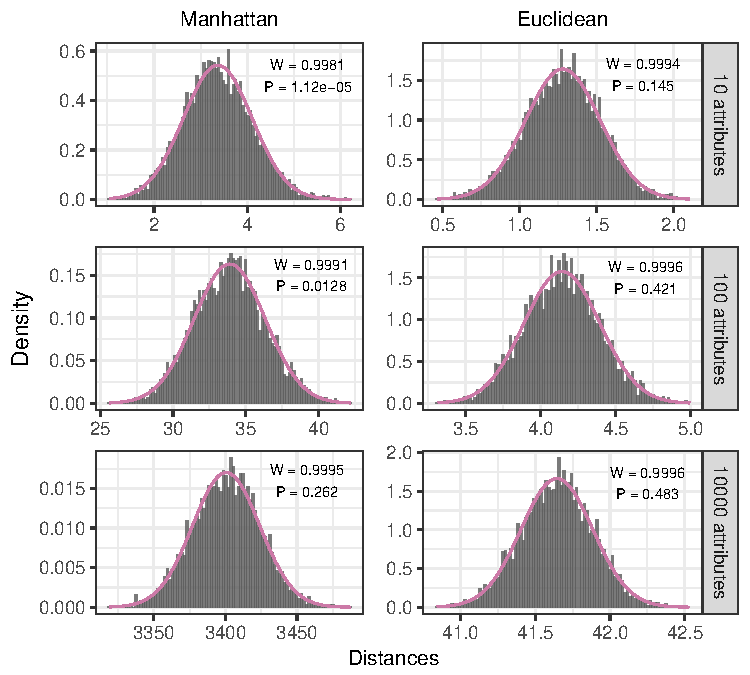
\includegraphics[width=0.98\textwidth]{central_limit_distances_uniform.pdf}}
	\caption{Convergence to normality of Manhattan and Euclidean distances. For each simulated distance distribution, we fixed $m=100$ instances and let $p=10,100,10000$. It is clear that convergence is rapid, and approximate normality can be safely assumed for even $p=10$.}\label{fig:central_limit_convergence}
\end{figure}

Although some p-values are significant at the 0.05 level for Manhattan ($q=1$), a visual inspection of the corresponding QQ-plots shown in Fig.~\ref{fig:qq-plots} indicate the normality assumption holds reasonably well.

\begin{figure}[H]
	\centering
	\framebox{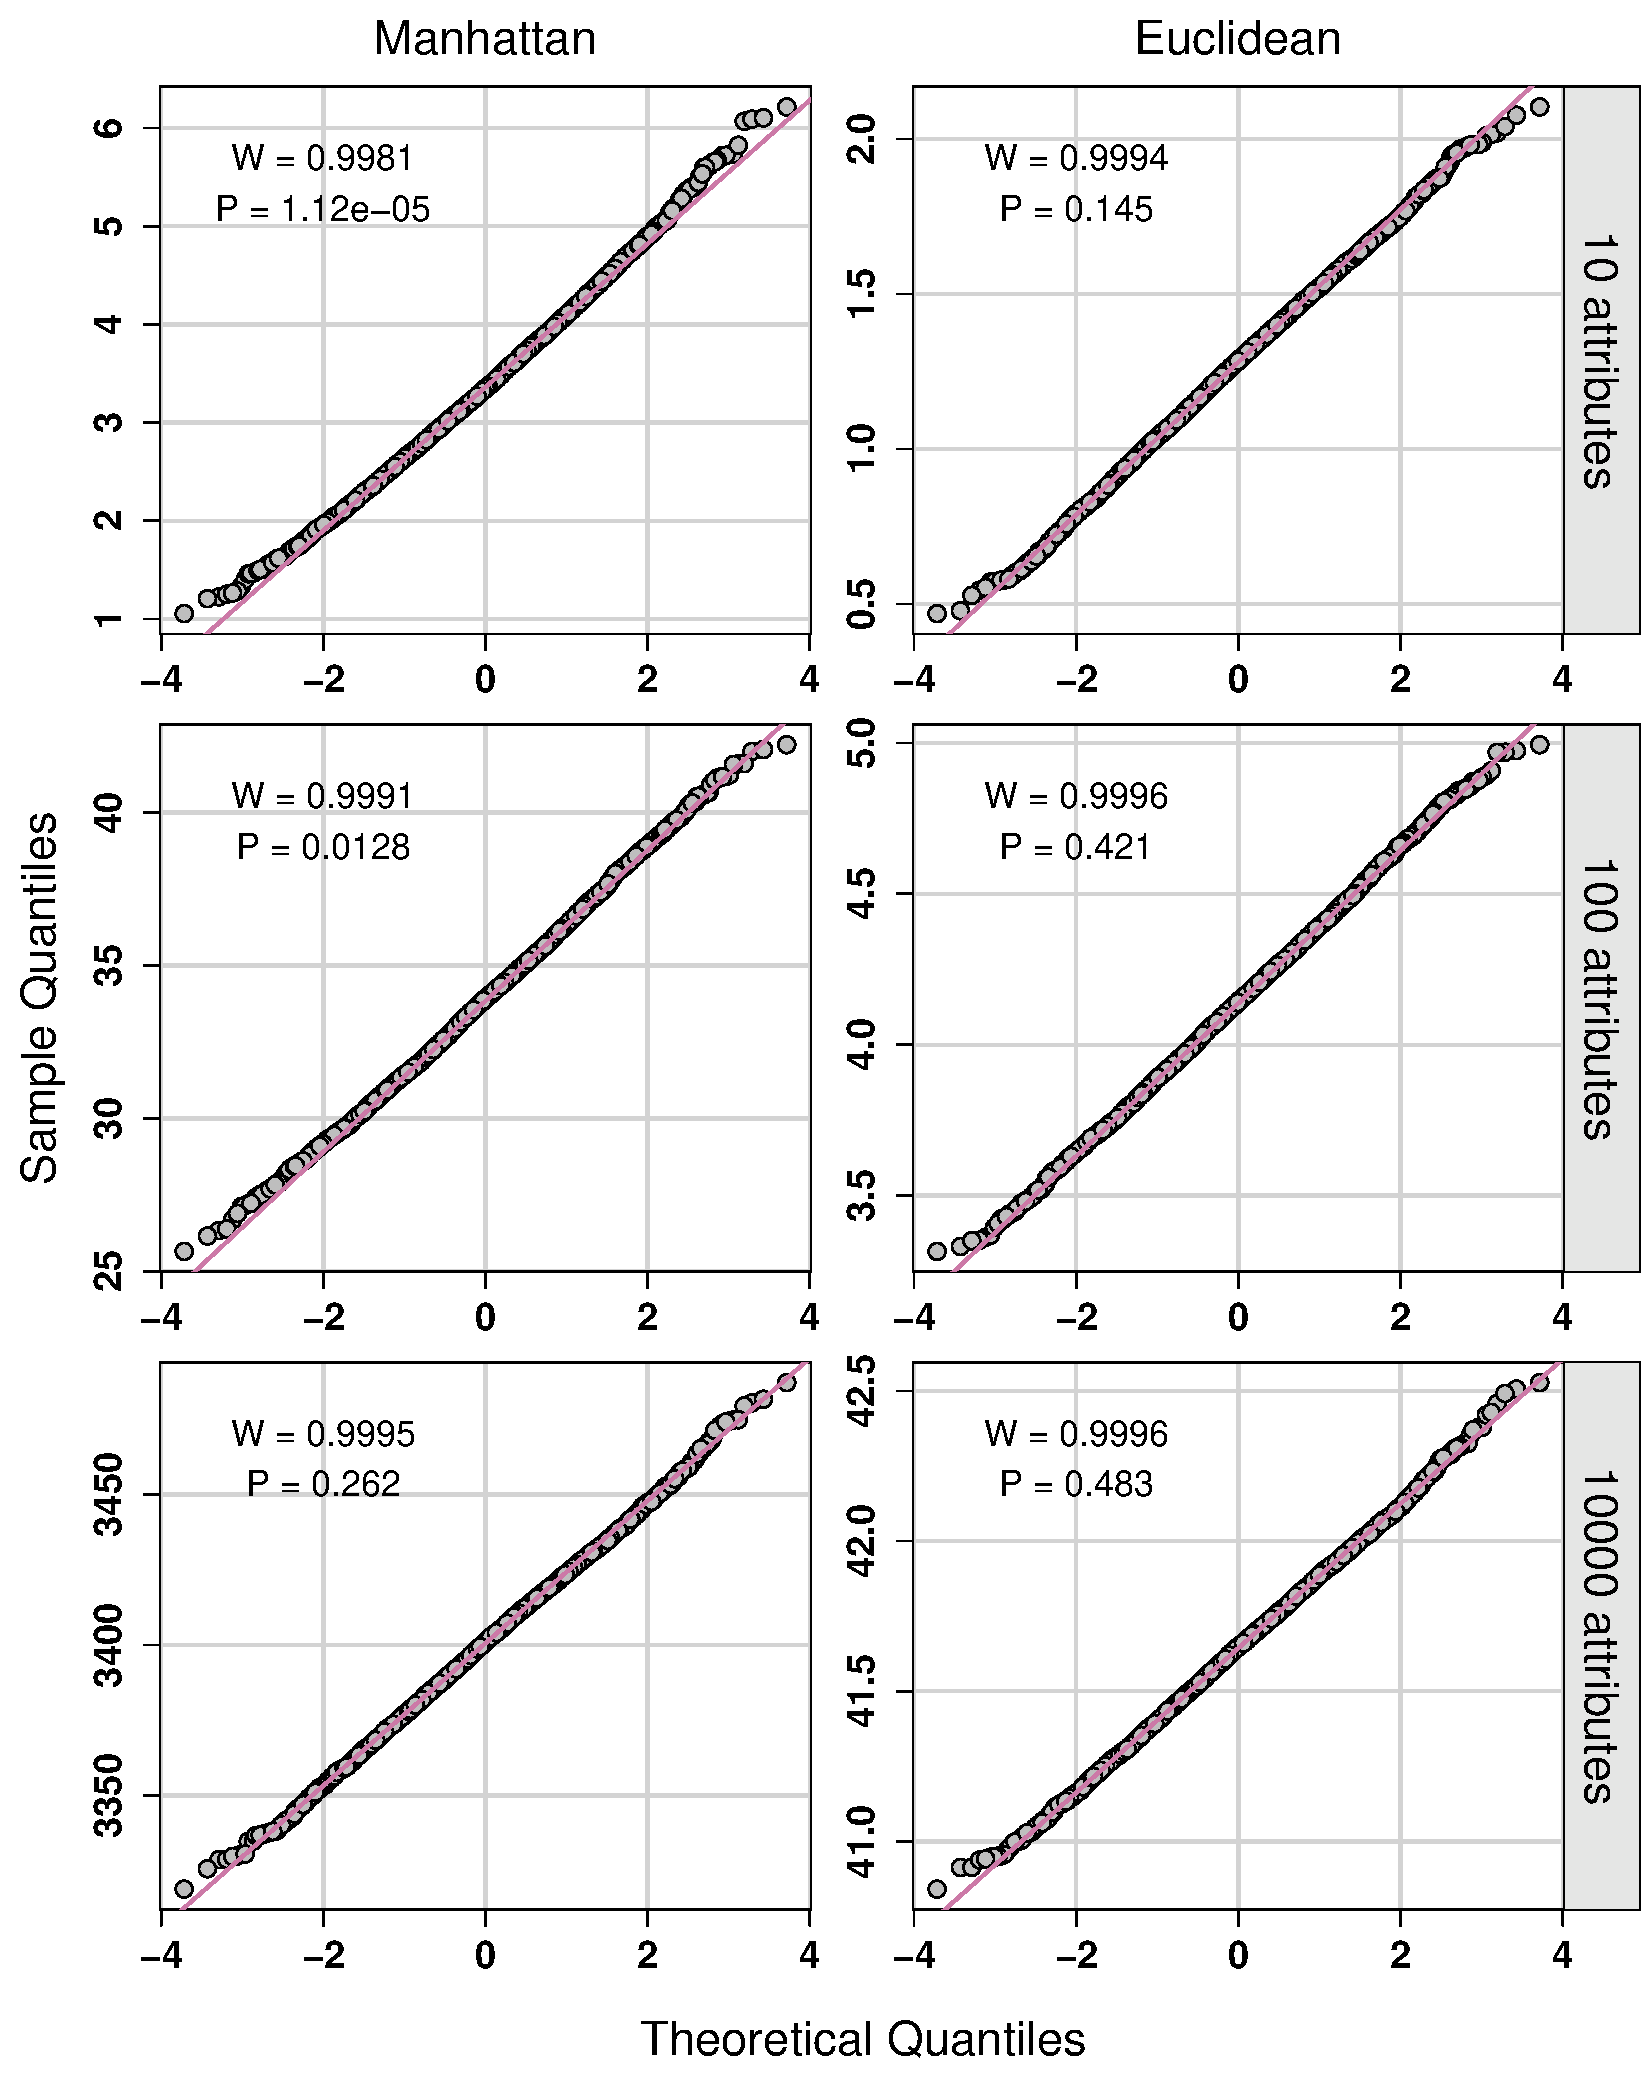
\includegraphics[width=0.98\textwidth]{qq-plots.pdf}}
	\caption{QQ-plots corresponding to the simulated distances in Fig.~\ref{fig:central_limit_convergence}. Although there are significant p-values for the case of Manhattan for $p=10,100$, it is clear that the assumption of normality is safe due to strong relationship between sample and theoretical quantiles.}\label{fig:qq-plots}
\end{figure}

%\begin{figure}[ht!]
%\centering
%		\framebox{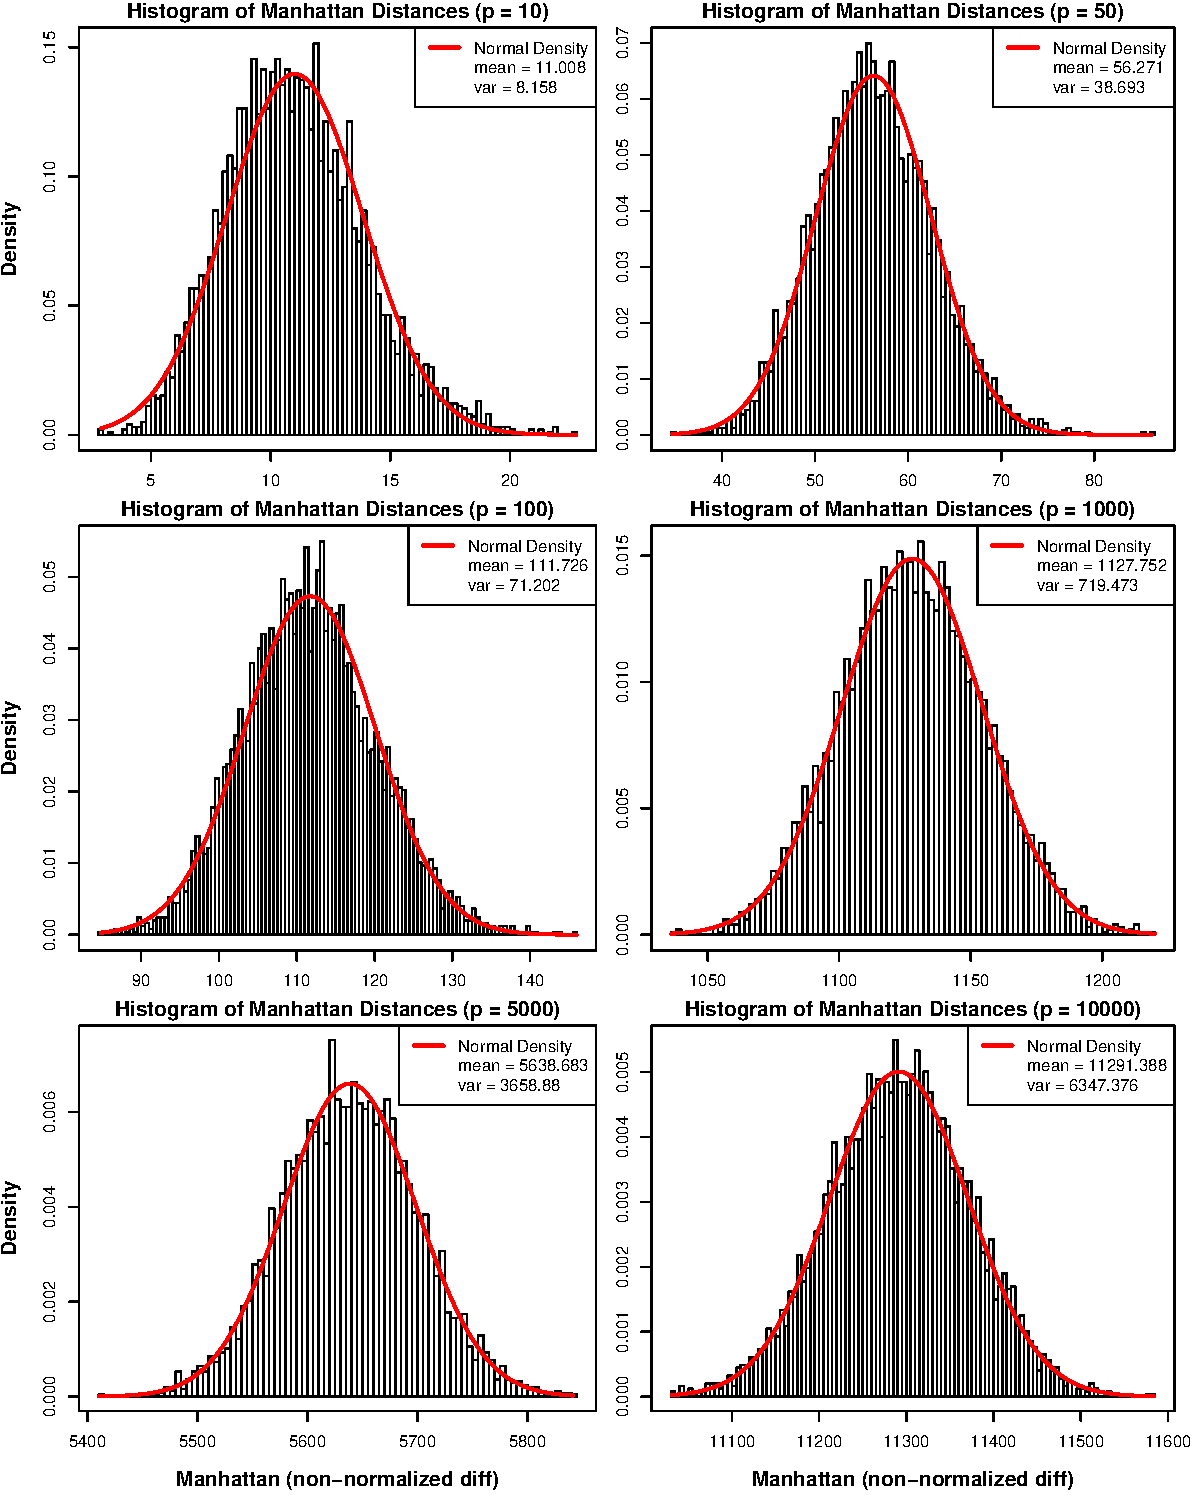
\includegraphics[width=0.95\textwidth]{central_limit_distances-Manhattan-Normal-diffstar.pdf}}
%		\caption{Convergence to normality of Manhattan distances between iid random normal instances. For each simulated distance distribution, we fixed $m=100$ instances but varied $p$ from 10 to 10000. It is clear that convergence is rapid, and approximate normality can be safely assumed for even $p=10$.}\label{fig:manhattanConverge}
%\end{figure} 

%\begin{figure}[ht!]
%\centering
%		\framebox{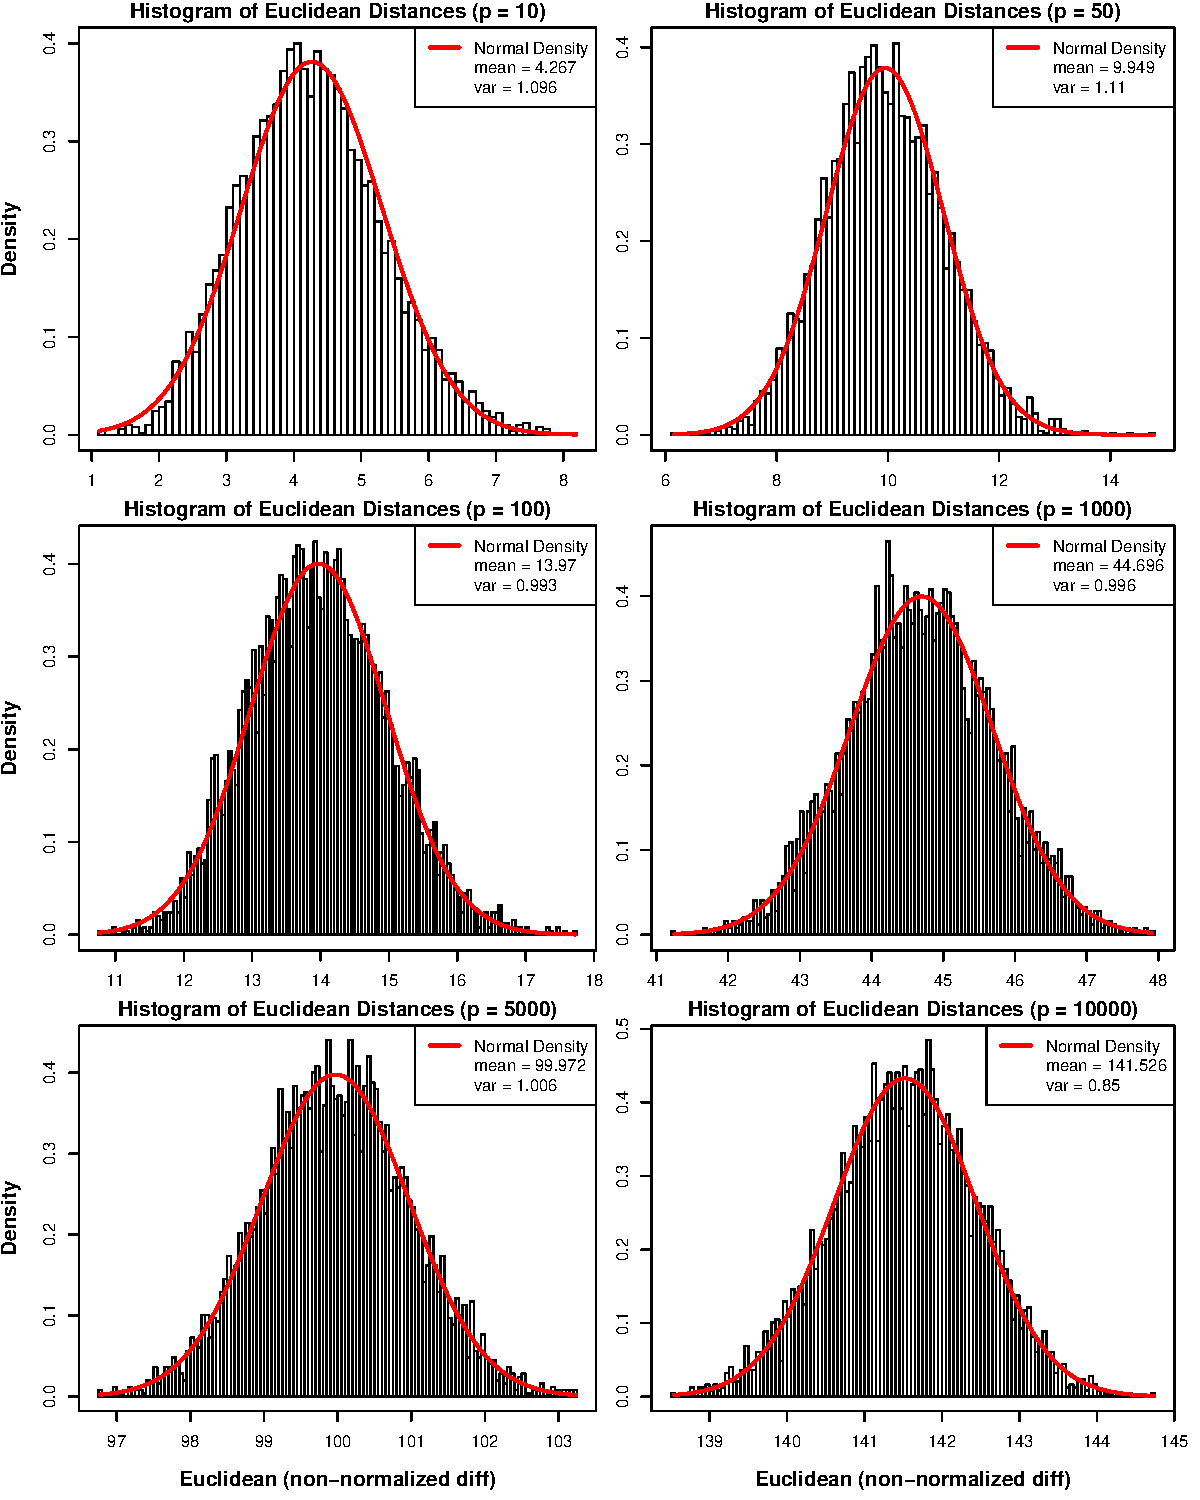
\includegraphics[width=0.95\textwidth]{central_limit_distances-Euclidean-Normal-diffstar.pdf}}
%		\caption{Convergence to normality of Euclidean distances between iid random normal instances. For each simulated distance distribution, we fixed $m=100$ instances but varied $p$ from 10 to 10000. It is clear that convergence is rapid, and approximate normality can be safely assumed for even $p=10$.}\label{fig:euclideanConverge}
%\end{figure}

For distance based learning methods, all pairwise distances are used to determine relative importances for attributes. The collection of all distances above the diagonal in an $m \times m$ distance matrix does not satisfy the independence assumption used in the previous derivations. This is because of the redundancy that is inherent to the distance matrix calculation. However, this collection is still asymptotically normal with mean and variance approximately equal to those given in Eq. \ref{eq:DqDeltaMethod}. In the next section, we assume actual data distributions in order to define more specific general formulas for standard $L_q$ and max-min normalized $L_q$ metrics. We also derive asymptotic moments for a new discrete metric in GWAS data and a new metric for time series correlation-based data, such as, resting-state fMRI.

%Hence, all fixed-radius methods will use a fixed radius that is some fraction of the expected pairwise distance for a given metric and data type. This implies that the probability of a fixed instance $j$ being within a fixed radius of a given instance $i$ can be parameterized by the expected pairwise distance and the variance of the pairwise distance. This probability is obtained by evaluating the normal cumulative distribution function (CDF), with corresponding mean and variance, at the quantile given by some function of the fixed radius. Therefore, we can derive the expected number of neighbors in the neighborhood of a fixed instance $i$. In other words, for sufficiently large data sets, the sample mean of the number of neighbors in a given neighborhood is well approximated by the product between the total number of possible neighbors and the expected probability of an instance being in a given neighborhood. The total number of possible neighbors for a fixed instance $i$ is always $m-1$, but this becomes approximately $\lfloor{\frac{m - 1}{2}}\rfloor$ when delineating between possible hits and misses for balanced data.

\section{Derivation of means and standard deviations for metrics and data distributions}

In this section, we begin by deriving general formulas for asymptotic means and variances of the $L_q$ distance given by Eq.~\ref{eq:D} for standard normal and standard uniform data. With our general formulas for continuous data, we compute moments associated with Manhattan ($L_1$) and Euclidean ($L_2$). We then consider the max-min normalized version of the $L_q$ distance, where the magnitude difference given by Eq.~\ref{eq:diff} is divided by the range of each feature $a$. Using Extreme Value Theory (EVT), we derive formulas for the moments of feature range in standard normal and standard uniform data. Transitioning into discrete data distributions relevant to GWAS, we derive asymptotic moments for two well known metrics and one new metric. In addition, we derive distance asymptotics for time series correlation-based data, such as, resting-state fMRI. 

\subsection{Distribution of \texorpdfstring{$|d_{ij}(a)|^q = |X_{ia} - X_{ja}|^q$}{}}

Suppose that $X_{ia}, X_{ja} \overset{iid}{\sim} \mathcal{F}_X(\mu_x,\sigma^2_x)$ and define $Z^q_a = |d_{ij}(a)|^q = |X_{ia} - X_{ja}|^q$, where $a \in \mathcal{A}$ and $|\mathcal{A}| = p$. In order to find the distribution of $Z^q_a$, we will use the following theorem given in \cite{freund2004}.

\begin{theorem}\label{thm:freund}
Let $f(x)$ be the value of the probability density of the continuous random variable $X$ at $x$. If the function given by $y = u(x)$ is differentiable and either increasing or decreasing for all values within the range of $X$ for which $f(x) \neq 0$, then, for these values of $x$, the equation $y = u(x)$ can be uniquely solved for $x$ to give $x = w(y)$, and for the corresponding values of $y$ the probability density of $Y = u(X)$ is given by

\[g(y) = f[w(y)] \cdot |w^\prime(y)| \quad \text{ provided } u^\prime(x) \neq 0\]

\noindent Elsewhere, $g(y) = 0$.
\end{theorem}

We have the following cases that result from solving for $X_{ja}$ in the equation given by $Z^q_a = |X_{ia} - X_{ja}|^q$:
\begin{itemize}
\item[(i)] Suppose that $X_{ja} = X_{ia} - \left(Z^q_a\right)^{1/q}$. Based on the iid assumption for $X_{ia}$ and $X_{ja}$, it follows from Thm. \ref{thm:freund} that the joint density function $g^{(1)}$ of $X_{ia}$ and $Z^q_a$ is given by
%
\begin{equation}
\begin{aligned}
g^{(1)}(x_{ia},z_a) &= f_X(x_{ia},x_{ja})\biggl|\frac{\partial x_{ja}}{\partial z_a}\biggr| \\
&= f_X(x_{ia})f_X(x_{ja})\biggl|\frac{-1}{q} \left(z^q_a\right)^{\frac{1}{q}-1}\biggr| \\
&= \frac{1}{q \left(z^q_a\right)^{1 - \frac{1}{q}}}f_X(x_{ia})f_X\left(x_{ia}-\left(z^q_a\right)^{1/q}\right), \quad z_a > 0
\end{aligned}
\end{equation}

The density function $f^{(1)}_{Z^q}$ of $Z^q_a$ is then defined as
%
\begin{equation}
\begin{aligned}
f^{(1)}_{Z^q}(z^q_a) &= \int_{-\infty}^{\infty} g^{(1)}(x_{ia},z^q_a)\text{d}x_{ia} \\
&= \frac{1}{q \left(z^q_a\right)^{1 - \frac{1}{q}}}\int_{-\infty}^{\infty} f_X(x_{ia})f_X\left(x_{ia}-\left(z^q_a\right)^{1/q}\right)\text{d}x_{ia}, \quad z_a > 0.
\end{aligned}
\end{equation}

\item[(ii)] Suppose that $X_{ja} = X_{ia} + \left(Z^q_a\right)^{1/q}$. Based on the iid assumption for $X_{ia}$ and $X_{ja}$, it follows from Thm. \ref{thm:freund} that the joint density function $g^{(2)}$ of $X_{ia}$ and $Z_a$ is given by
%
\begin{equation}
\begin{aligned}
g^{(2)}(x_{ia},z_a) &= f_X(x_{ia},x_{ja})\biggl|\frac{\partial x_{ja}}{\partial z_a}\biggr| \\
&= f_X(x_{ia})f_X(x_{ja})\biggl|\frac{1}{q} \left(z^q_a\right)^{\frac{1}{q}-1}\biggr| \\
&= \frac{1}{q \left(z^q_a\right)^{1 - \frac{1}{q}}}f_X(x_{ia})f_X\left(x_{ia}-\left(z^q_a\right)^{1/q}\right), \quad z_a > 0.
\end{aligned}
\end{equation}

The density function $f^{(2)}_{Z^q}$ of $Z^q_a$ is then defined as
%
\begin{equation}
\begin{aligned}
f^{(2)}_{Z^q}(z^q_a) &= \int_{-\infty}^{\infty} g^{(2)}(x_{ia},z^q_a)\text{d}x_{ia} \\
&= \frac{1}{q \left(z^q_a\right)^{1 - \frac{1}{q}}}\int_{-\infty}^{\infty} f_X(x_{ia})f_X\left(x_{ia}+\left(z^q_a\right)^{1/q}\right)\text{d}x_{ia}, \quad z_a > 0.
\end{aligned}
\end{equation}
\end{itemize}

Let $F_{Z^q}$ denote the distribution function of the random variable $Z^q_a$. Furthermore, we define the events $E^{(1)}$ and $E^{(2)}$ as
%
\begin{equation}\label{eq:E(1)}
E^{(1)} = \bigl\{|X_{ia}-X_{ja}|^q \leq z^q_a | X_{ja} = X_{ia} - \left(Z^q_a\right)^{1/q}\bigr\}
\end{equation}
%
and
%
\begin{equation}\label{eq:E(2)}
E^{(2)} = \bigl\{|X_{ia}-X_{ja}|^q \leq z^q_a | X_{ja} = X_{ia} + \left(Z^q_a\right)^{1/q}\bigr\}.
\end{equation}

Then it follows from fundamental rules of probability that
%
\begin{equation}\label{eq:DqCDF}
\begin{aligned}
F_{Z^q}(z^q_a) &= \text{P}\left[Z^q_a \leq z^q_a\right] \\
&= \text{P}\left[|X_{ia} - X_{ja}|^q \leq z^q_a\right] \\
&= \text{P}\left[E^{(1)} \cup E^{(2)}\right] \\
&= \text{P}\bigl[E^{(1)}\bigr] + \text{P}\bigl[E^{(2)}\bigr] - \text{P}\bigl[E^{(1)} \cap E^{(2)}\bigr] \\
&= \text{P}\bigl[E^{(1)}\bigr] + \text{P}\bigl[E^{(2)}\bigr] \\
&= \int_{-\infty}^{z^q_a} f^{(1)}_{Z^q}(t) \text{d}t + \int_{-\infty}^{z^q_a} f^{(2)}_{Z^q}(t) \text{d}t \\
&= \int_{-\infty}^{z^q_a} \left(f^{(1)}_{Z^q}(t) + f^{(2)}_{Z^q}(t)\right) \text{d}t \\
&= \frac{1}{q \left(z^q_a\right)^{1 - \frac{1}{q}}}\int_{-\infty}^{z^q_a} \left(\int_{-\infty}^{\infty}f_X(x_{ia})\left[f_X(x_{ia} - t) + f_X(x_{ia} + t)\right] \text{d}x_{ia}\right)\text{d}t, \quad z_a > 0.
\end{aligned}
\end{equation}

It follows directly from the result in Eq. \ref{eq:DqCDF} that the density function of the random variable $Z^q_a$ is given by
%
\begin{equation}\label{eq:DqPDF}
\begin{aligned}
f_{Z^q}(z^q_a) &= \frac{\partial}{\partial z^q_a} F_{Z^q}(z^q_a) \\
&= \frac{1}{q \left(z^q_a\right)^{1 - \frac{1}{q}}}\int_{-\infty}^{\infty} f_X(x_{ia})\left[f_X\left(x_{ia} - \left(z^q_a\right)^{1/q}\right) + f_X\left(x_{ia} + \left(z^q_a\right)^{1/q}\right)\right] \text{d}x_{ia},
\end{aligned}
\end{equation}
%
where $z_a > 0$.

Using Eq. \ref{eq:DqPDF}, we can compute the mean and variance of the random variable $Z^q_a$ as
%
\begin{equation}\label{eq:1DDqMean}
\mu_{z^q} = \int_{-\infty}^{\infty} z^q_a f_{Z^q}(z^q_a) \text{d}z^q_a
\end{equation}
%
and 
%
\begin{equation}\label{eq:1DDqVar}
\sigma^2_{z^q} = \int_{-\infty}^{\infty} \left(z^q_a\right)^2 f_{Z^q}(z^q_a) \text{d}z^q_a - \mu^2_{z^q}.
\end{equation}

It follows immediately from Eqs. \ref{eq:1DDqMean} and \ref{eq:1DDqVar} and the Classical Central Limit Theorem (CCLT) that
%
\begin{equation}\label{eq:DqDistr}
\left(D^{(q)}_{ij}\right)^q = \sum_{a \in \mathcal{A}} Z^q_a = \sum_{a \in \mathcal{A}} |X_{ia} - X_{ja}|^q \overset{.}{\sim} \mathcal{N}\left(\mu_{z^q}p,\sigma^2_{z^q}p\right).
\end{equation}

Applying the result given in Eq. \ref{eq:DqDeltaMethod}, the distribution of $D^{(q)}_{ij}$ is given by
%
\begin{equation}\label{eq:DDistr}
D^{(q)}_{ij} \overset{.}{\sim} \mathcal{N}\left(\left(\mu_{z^q}p\right)^{1/q},\frac{\sigma^2_{z^q}p}{q^2\left(\mu_{z^q}p\right)^{2\left(1 - \frac{1}{q}\right)}}\right), \quad \mu_{z^q} > 0
\end{equation}
%
with improved estimate of the mean for $q=2$ given by Eq. \ref{eq:DqImprovedExplained}.

\subsubsection{Standard normal data}

If $X_{ia},X_{ja} \overset{iid}{\sim} \mathcal{N}(0,1)$, then the marginal density functions with respect to $X$ for $X_{ia}$, $X_{ia} - \left(Z^q_a\right)^{1/q}$, and $X_{ia} + \left(Z^q_a\right)^{1/q}$ are defined as
%
\begin{equation}\label{eq:normalXmarg}
f_X(x_{ia}) = \frac{1}{\sqrt{2\pi}}e^{-\frac{1}{2}x^2_{ia}},
\end{equation}
%
\begin{equation}\label{eq:normalXMinusZmarg}
f_X\left(x_{ia} - \left(z^q_a\right)^{1/q}\right) = \frac{1}{\sqrt{2\pi}}e^{-\frac{1}{2}\left(x_{ia} - \left(z^q_a\right)^{1/q}\right)^2}, \quad z_a > 0, \text{ and}
\end{equation}
%
\begin{equation}\label{eq:normalXPlusZmarg}
f_X\left(x_{ia} + \left(z^q_a\right)^{1/q}\right) = \frac{1}{\sqrt{2\pi}}e^{-\frac{1}{2}\left(x_{ia} + \left(z^q_a\right)^{1/q}\right)^2}, \quad z_a > 0.
\end{equation}

Substituting the results given by Eqs. \ref{eq:normalXmarg}-\ref{eq:normalXPlusZmarg} into Eq. \ref{eq:DqPDF} and completing the square on $x_{ia}$ in the exponents, we have
%
%\begin{equation}\label{eq:normalPDF}
\begin{align}\label{eq:normalPDF}
  \begin{split}
  f_{Z^q}(z^q_a) &= \frac{1}{2 q \pi \left(z^q_a\right)^{1 - \frac{1}{q}}} e^{-\frac{1}{4}\left(z^q_a\right)^{2    /q}}\int_{-\infty}^{\infty} \biggl(e^{-\frac{1}{2}\left[\sqrt{2}x_{ia} - \frac{\sqrt{2}}{2}\left(z^q_a\right)^{1/q}\right]^2} \\
&\hspace{2in} + e^{-\frac{1}{2}\left[\sqrt{2}x_{ia} + \frac{\sqrt{2}}{2}\left(z^q_a\right)^{1/q}\right]^2}\biggr) \text{d}x_{ia}
\end{split} 
\\
&= \frac{1}{2 q \sqrt{\pi} \left(z^q_a\right)^{1 - \frac{1}{q}}} e^{-\frac{1}{4}\left(z^q_a\right)^{2/q}} \int_{-\infty}^{\infty}\frac{1}{\sqrt{2\pi}} \left(e^{-\frac{1}{2}u^2} + e^{-\frac{1}{2}u^2}\right) \text{d}u \\
&= \frac{1}{2 q \sqrt{\pi} \left(z^q_a\right)^{1 - \frac{1}{q}}} e^{-\frac{1}{4}\left(z^q_a\right)^{2/q}} (1 + 1) \\
&= \frac{1}{q \sqrt{\pi}}\left(z^q_a\right)^{\frac{1}{q} - 1} e^{-\frac{1}{4}\left(z^q_a\right)^{2/q}} \\
&= \frac{\frac{2}{q}}{\left(2^q\right)^{1/q} \Gamma\left(\frac{\frac{1}{q}}{\frac{2}{q}}\right)}\left(z^q_a\right)^{\frac{1}{q} - 1} e^{-\left(\frac{z^q_a}{2^q}\right)^{2/q}}.
\end{align}
%\end{equation}

The density function given by Eq. \ref{eq:normalPDF} is a Generalized Gamma density with parameters $b = \frac{2}{q}$, $c = 2^q$, and $d = \frac{1}{q}$. This distribution has mean and variance given by
%
\begin{equation}\label{eq:1DnormalDqMean}
\begin{aligned}
\mu_{z^q} &= \frac{c\Gamma\left(\frac{d+1}{b}\right)}{\Gamma\left(\frac{d}{b}\right)} \\
&= \frac{2^q \Gamma\left(\frac{q + 1}{2}\right)}{\sqrt{\pi}}
\end{aligned}
\end{equation}
%
and
%
\begin{equation}\label{eq:1DnormalDqVar}
\begin{aligned}
\sigma^2_{z^q} &= c^2\left[\frac{\Gamma\left(\frac{d+2}{b}\right)}{\Gamma\left(\frac{d}{b}\right)} - \left(\frac{\Gamma\left(\frac{d+1}{b}\right)}{\Gamma\left(\frac{d}{b}\right)}\right)^2\right] \\
&= 4^{q}\left[\frac{\Gamma\left(q + \frac{1}{2}\right)}{\sqrt{\pi}} - \frac{\Gamma^2\left(\frac{1}{2}q + \frac{1}{2}\right)}{\pi}\right].
\end{aligned}
\end{equation}

By linearity of the expected value and variance operators under the iid assumption, Eqs. \ref{eq:1DnormalDqMean} and \ref{eq:1DnormalDqVar} allow the $p\text{-dimensional}$ mean and variance of the $D^{(q)}_{ij}$ distribution to be computed directly as
%
\begin{equation}\label{eq:normalDqMean}
\mu_{\left(D^{(q)}_{ij}\right)^q} = \text{E}\left[\left(D^{(q)}_{ij}\right)^q\right] = \text{E}\left(\sum_{a \in \mathcal{A}} Z^q_a\right) = \sum_{a \in \mathcal{A}} \text{E}\left(Z^q_a\right) = \sum_{a \in \mathcal{A}} \frac{2^q \Gamma\left(\frac{q + 1}{2}\right)}{\sqrt{\pi}} = \frac{2^q\Gamma\left(\frac{q + 1}{2}\right)}{\sqrt{\pi}}p
\end{equation}
%
and
%
\begin{equation}\label{eq:normalVar}
\begin{split}
\sigma^2_{\left(D^{(q)}_{ij}\right)^q} = \text{Var}\left[\left(D^{(q)}_{ij}\right)^q\right] &= \text{Var}\left(\sum_{a \in \mathcal{A}} Z^q_a\right) \\
&= \sum_{a \in \mathcal{A}} \text{Var}\left(Z^q_a\right) \\
&= \sum_{a \in \mathcal{A}} 4^{q}\left[\frac{\Gamma\left(q + \frac{1}{2}\right)}{\sqrt{\pi}} - \frac{\Gamma^2\left(\frac{1}{2}q + \frac{1}{2}\right)}{\pi}\right] \\
&= 4^{q}\left[\frac{\Gamma\left(q + \frac{1}{2}\right)}{\sqrt{\pi}} - \frac{\Gamma^2\left(\frac{1}{2}q + \frac{1}{2}\right)}{\pi}\right]p.
\end{split}
\end{equation}

Therefore, the asymptotic distribution of $D^{(q)}_{ij}$ for standard normal data is
%
\begin{equation}\label{eq:normalDistr}
\mathcal{N}\left(\left(2^q\frac{\Gamma\left(\frac{q + 1}{2}\right)}{\sqrt{\pi}}p\right)^{1/q},
\frac{4^q p}{q^2 \left(\frac{2^q \Gamma\left(\frac{1}{2}q + \frac{1}{2}\right)}{\sqrt{\pi}}p\right)^{2\left(1 - \frac{1}{q}\right)}}\left[\frac{\Gamma\left(q + \frac{1}{2}\right)}{\sqrt{\pi}} - \frac{\Gamma^2\left(\frac{1}{2}q + \frac{1}{2}\right)}{\pi}\right]\right).
\end{equation}

\subsubsection{Standard uniform data}

If $X_{ia},X_{ja} \overset{iid}{\sim} \mathcal{U}(0,1)$, then the marginal density functions with respect to $X$ for $X_{ia}$, $X_{ia} - \left(Z^q_a\right)^{1/q}$, and $X_{ia} + \left(Z^q_a\right)^{1/q}$ are defined as
%
\begin{equation}\label{eq:uniformXmarg}
f_X(x_{ia}) = 1, \quad 0 \leq x_{ia} \leq 1
\end{equation}
%
\begin{equation}\label{eq:uniformXMinusZmarg}
f_X\left(x_{ia} - \left(z^q_a\right)^{1/q}\right) = 1, \quad 0 \leq x_{ia} - \left(z^q_a\right)^{1/q} \leq 1, \text{ and}
\end{equation}
%
\begin{equation}\label{eq:uniformXPlusZmarg}
f_X\left(x_{ia} + \left(z^q_a\right)^{1/q}\right) = 1, \quad 0 \leq x_{ia} + \left(z^q_a\right)^{1/q} \leq 1.
\end{equation}

Substituting the results given by Eqs. \ref{eq:uniformXmarg}-\ref{eq:uniformXPlusZmarg} into Eq. \ref{eq:DqPDF}, we have
%
\begin{equation}\label{eq:uniformDqPDF}
\begin{aligned}
f_{Z^q}(z^q_a) &= \frac{1}{q\left(z^q_a\right)^{1 - \frac{1}{q}}}\int_{-\infty}^{\infty}f_X(x_{ia})\left[f_X\left(x_{ia} - \left(z^q_a\right)^{1/q}\right) + f_X\left(x_{ia} + \left(z^q_a\right)^{1/q}\right)\right]\text{d}x_{ia},\\
& \hspace{4in} 0 < z_a \leq 1\\
&= \frac{1}{q\left(z^q_a\right)^{1 - \frac{1}{q}}}\int_{0}^{1}[f_X(x_{ia} - \left(z^q_a\right) + f_X\left(x_{ia} + \left(z^q_a\right)^{1/q}\right)]\text{d}x_{ia}, \quad 0 < z_a \leq 1 \\
&= \frac{1}{q\left(z^q_a\right)^{1 - \frac{1}{q}}}\int_{\left(z^q_a\right)}^{1}1\text{d}x_{ia} + \int_{0}^{1 - \left(z^q_a\right)}1\text{d}x_{ia}, \quad 0 < z_a \leq 1 \\
&= \frac{1}{q\left(z^q_a\right)^{1 - \frac{1}{q}}}\left[\left(1 - \left(z^q_a\right)\right) + \left(1 - \left(z^q_a\right)\right)\right], \quad 0 < z_a \leq 1 \\
&= \frac{1}{q} \cdot 2 \left(z^q_a\right)^{\frac{1}{q} - 1}\left[1 - \left(z^q_a\right)^{1/q}\right]^{2 - 1}, \quad 0 < z_a \leq 1.
\end{aligned}
\end{equation}

The density given by Eq. \ref{eq:uniformDqPDF} is a Kumaraswamy density with parameters $b = \frac{1}{q}$ and $c = 2$ with moment generating function (MGF) given by
%
\begin{equation}\label{eq:uniformDqMGF}
\begin{aligned}
M_n &=  \frac{c\Gamma\left(1 + \frac{n}{b}\right) \Gamma(c)}{\Gamma\left(1 + c + \frac{n}{b}\right)}\\
&= \frac{2}{(nq + 2)(nq + 1)}.
\end{aligned}
\end{equation}

Using the MGF given by Eq. \ref{eq:uniformDqMGF}, the mean and variance of $Z^q_a$ are computed as
%
\begin{equation}\label{eq:1DuniformDqMean}
\mu_{z^q} = \frac{2}{(q + 2)(q + 1)}
\end{equation}
%
and
%
\begin{equation}\label{eq:1DuniformDqVar}
\sigma^2_{z^q} = \frac{1}{(q + 1)(2q + 1)} - \left(\frac{2}{(q + 2)(q + 1)}\right)^2.
\end{equation}

By linearity of the expected value and variance operators under the iid assumption, Eqs. \ref{eq:uniformDqMean} and \ref{eq:uniformDqVar} allow the $p \text{-dimensional}$ mean and variance of the $\left(D^{(q)}_{ij}\right)^q$ distribution to be computed directly as
%
\begin{equation}\label{eq:uniformDqMean}
\begin{split}
\mu_{\left(D^{(q)}_{ij}\right)^q} = \text{E}\left[\left(D^{(q)}_{ij}\right)^q\right] &= \text{E}\left(\sum_{a \in \mathcal{A}}Z^q_a\right) \\
&= \sum_{a \in \mathcal{A}} \text{E}(Z^q_a) \\
&= \sum_{a \in \mathcal{A}} \frac{2}{(q + 2)(q + 1)} \\
&= \frac{2p}{(q + 2)(q + 1)}
\end{split}
\end{equation}
%
and
%
\begin{equation}\label{eq:uniformDqVar}
\begin{split}
\sigma^2_{\left(D^{(q)}_{ij}\right)^q} = \text{Var}\left[\left(D^{(q)}_{ij}\right)^q\right] &= \text{Var}\left(\sum_{a \in \mathcal{A}} Z^q_a\right) \\
&= \sum_{a \in \mathcal{A}} \text{Var}\left(Z^q_a\right) \\
&= \sum_{a \in \mathcal{A}} \left[\frac{1}{(q + 1)(2q + 1)} - \left(\frac{2}{(q + 2)(q + 1)}\right)^2\right] \\
&= \left[\frac{1}{(q + 1)(2q + 1)} - \left(\frac{2}{(q + 2)(q + 1)}\right)^2\right]p.
\end{split}
\end{equation}

Therefore, the asymptotic distribution of $D^{(q)}_{ij}$ for standard uniform data is
%
\begin{equation}\label{eq:uniformDistr}
\begin{split}
\mathcal{N}{\text{\LARGE $\Biggl($}}& \left(\frac{2p}{(q + 2)(q + 1)}\right)^{1/q}, \\
& \frac{p}{q^2\left(\frac{2p}{(q + 2)(q + 1)}\right)^{2\left(1 - \frac{1}{q}\right)}}\left[\frac{1}{(q + 1)(2q + 1)} - \left(\frac{2}{(q + 2)(q + 1)}\right)^2\right]{\text{\LARGE $\Biggr)$}}.
\end{split}
\end{equation}

\subsection{Manhattan \texorpdfstring{($q=1$)}{}}

With our general formulas for the asymptotic mean and variance given by Eqs. \ref{eq:normalDistr} and \ref{eq:uniformDistr} for any value of $q \in \mathbb{Z}^+$, we can simply substitute a particular value of $q$ in order to determine the asymptotic distribution of the corresponding distance metric $D^{(q)}_{ij}$. We demonstrate this with the example of the Manhattan ($q=1$) metric for standard normal and standard uniform data.

\subsubsection{Standard normal data}

Using the mean given by Eq. \ref{eq:normalDistr} and substituting $q=1$, we have the following for standard normal data
%
\begin{equation}\label{eq:normalManMean}
\begin{aligned}
\text{E}\left(D^{(1)}_{ij}\right) &= \left(2\frac{\Gamma\left(\frac{1 + 1}{2}\right)}{\sqrt{\pi}}p\right)^{1/1} \\
&= \frac{2p}{\sqrt{\pi}}\Gamma(1) \\
&= \frac{2p}{\sqrt{\pi}}.
\end{aligned}
\end{equation}

Similarly, the variance of $D^{(1)}_{ij}$ is given by
%
\begin{equation}\label{eq:normalManVar}
\begin{aligned}
\text{Var}\left(D^{(1)}_{ij}\right) &= \frac{4^1p}{1^2\left(\frac{2^1\Gamma\left(\frac{1}{2}(1) + \frac{1}{2}\right)}{\sqrt{\pi}}p\right)^{2\left(1 - \frac{1}{1}\right)}}\left[\frac{\Gamma\left(1 + \frac{1}{2}\right)}{\sqrt{\pi}} - \frac{\Gamma^2\left(\frac{1}{2}(1) + \frac{1}{2}\right)}{\pi}\right] \\
&= \frac{4p}{1}\left[\frac{\frac{1}{2}\Gamma\left(\frac{1}{2}\right)}{\sqrt{\pi}} - \frac{\Gamma^2(1)}{\pi}\right] \\
&= 4p\left[\frac{1}{2} - \frac{1}{\pi}\right] \\
&= \frac{2(\pi - 2)p}{\pi}.
\end{aligned}
\end{equation}

\subsubsection{Standard uniform data}

Using the mean given by Eq. \ref{eq:uniformDistr} and substituting $q=1$, we have the following for standard uniform data
%
\begin{equation}\label{eq:uniformManMean}
\begin{aligned}
\text{E}\left(D^{(1)}_{ij}\right) &= \left(\frac{2p}{(1+2)(1+1)}\right)^{1/1} \\
&= \frac{2p}{6} \\
&= \frac{p}{3}.
\end{aligned}
\end{equation}

Similarly, the variance of $D^{(1)}_{ij}$ is given by
%
\begin{equation}\label{eq:uniformManVar}
\begin{aligned}
\text{Var}\left(D^{(1)}_{ij}\right) &= \frac{p}{1^2\left(\frac{2p}{(1 + 2)(1 + 1)}\right)^{2\left(1 - \frac{1}{1}\right)}}\left[\frac{1}{(1 + 1)(2(1) + 1)} - \left(\frac{2}{(1 + 2)(1 + 1)}\right)^2\right] \\
&= p\left[\frac{1}{6} - \frac{1}{9}\right] \\
&= \frac{p}{18}.
\end{aligned}
\end{equation}

\subsection{Euclidean \texorpdfstring{($q=2$)}{}}

Analogous to the previous section, we demonstrate the usage of Eqs. \ref{eq:normalDistr} and \ref{eq:uniformDistr} for the Euclidean ($q=2$) metric for standard normal and standard uniform data.

\subsubsection{Standard normal data}

Using the mean given by Eq. \ref{eq:normalDistr} and substituting $q=2$, we have the following for standard normal data
%
\begin{equation}\label{eq:normalEucMean}
\begin{aligned}
\text{E}\left(D^{(2)}_{ij}\right) &= \left(2\frac{\Gamma\left(\frac{2 + 1}{2}\right)}{\sqrt{\pi}}p\right)^{1/2} \\
&= \left(\frac{2p}{\sqrt{\pi}}\Gamma\left(\frac{3}{2}\right)\right)^{1/2} \\
&= \sqrt{2p}.
\end{aligned}
\end{equation}

Similarly, the variance of $D^{(2)}_{ij}$ is given by
%
\begin{equation}\label{eq:normalEucVar}
\begin{aligned}
\text{Var}\left(D^{(1)}_{ij}\right) &= \frac{4^2p}{2^2\left(\frac{2^2\Gamma\left(\frac{1}{2}(2) + \frac{1}{2}\right)}{\sqrt{\pi}}p\right)^{2\left(1 - \frac{1}{2}\right)}}\left[\frac{\Gamma\left(2 + \frac{1}{2}\right)}{\sqrt{\pi}} - \frac{\Gamma^2\left(\frac{1}{2}(2) + \frac{1}{2}\right)}{\pi}\right] \\
&= \frac{16p}{4\left(\frac{4\Gamma\left(\frac{3}{2}\right)}{\sqrt{\pi}}p\right)}\left[\frac{\Gamma\left(\frac{5}{2}\right)}{\sqrt{\pi}} - \frac{\Gamma^2\left(\frac{3}{2}\right)}{\pi}\right] \\
&= 2\left[\frac{3}{4} - \frac{1}{4}\right] \\
&= 1.
\end{aligned}
\end{equation}

For the case in which the number of attributes $p$ is small, an improved estimate of the mean is given by Eq. \ref{eq:DqImprovedExplained}. The lower dimensional estimate of the mean is as follows
%
\begin{equation}\label{eq:normalEucMeanImproved}
\begin{aligned}
\text{E}\left(D^{(2)}_{ij}\right) &= \left(2\frac{\Gamma\left(\frac{2 + 1}{2}\right)}{\sqrt{\pi}}p - 1\right)^{1/2} \\
&= \left(\frac{2p}{\sqrt{\pi}}\Gamma\left(\frac{3}{2}\right) - 1\right)^{1/2} \\
&= \sqrt{2p - 1}.
\end{aligned}
\end{equation}

For high dimensional data sets, such as gene expression, rs-fMRI, or GWAS, it is clear that the magntiude of $p$ will be sufficient to use Eq. \ref{eq:normalEucMean} since $\sqrt{2p} \approx \sqrt{2p - 1}$ in that case.

\subsubsection{Standard uniform data}

Using the mean given by Eq. \ref{eq:uniformDistr} and substituting $q=2$, we have the following for standard uniform data
%
\begin{equation}\label{eq:uniformEucMean}
\begin{aligned}
\text{E}\left(D^{(2)}_{ij}\right) &= \left(\frac{2p}{(2+2)(2+1)}\right)^{1/2} \\
&= \left(\frac{2p}{12}\right)^{1/2} \\
&= \sqrt{\frac{p}{6}}.
\end{aligned}
\end{equation}

Similarly, the variance of $D^{(2)}_{ij}$ is given by
%
\begin{equation}\label{eq:uniformEucVar}
\begin{aligned}
\text{Var}\left(D^{(2)}_{ij}\right) &= \frac{p}{2^2\left(\frac{2p}{(2 + 2)(2 + 1)}\right)^{2\left(1 - \frac{1}{2}\right)}}\left[\frac{1}{(2 + 1)(2(2) + 1)} - \left(\frac{2}{(2 + 2)(2 + 1)}\right)^2\right] \\
&= \frac{3}{2}\left[\frac{1}{15} - \frac{1}{36}\right] \\
&= \frac{7}{120}.
\end{aligned}
\end{equation}

For the case in which the number of attributes $p$ is small, an improved estimate of the mean is given by Eq. \ref{eq:DqImprovedExplained}. The lower dimensional estimate of the mean is as follows
%
\begin{equation}\label{eq:uniformEucMeanImproved}
\begin{aligned}
\text{E}\left(D^{(2)}_{ij}\right) &= \left(\frac{2p}{(2+2)(2+1)} - \frac{7}{120}\right)^{1/2} \\
&= \left(\frac{2p}{12} - \frac{7}{120}\right)^{1/2} \\
&= \sqrt{\frac{p}{6} - \frac{7}{120}}.
\end{aligned}
\end{equation}

For high dimensional data sets, such as gene expression, rs-fMRI, or GWAS, it is clear that the magntiude of $p$ will be sufficient to use Eq. \ref{eq:normalEucMean} since $\sqrt{\frac{p}{6}} \approx \sqrt{\frac{p}{6} - \frac{7}{120}}$ in that case.

\subsection{Distribution of attribute extremes}

For Relief-based methods \cite{robnik2003,urbanowiczReliefReview2018}, the standard numeric diff metric is given by
%
\begin{equation}\label{eq:normDiff}
d^{\text{num}}_{ij}(a) = \text{diff}(a,(i,j)) = \frac{|X_{ia} - X_{ja}|}{\text{max}(a) - \text{min}(a)},
\end{equation}

\noindent where $\text{max}(a) = \displaystyle \max_{k \in \mathcal{I}}\{X_{ka}\}$, $\text{min}(a) = \displaystyle \min_{k \in \mathcal{I}}\{X_{ka}\}$, and $\mathcal{I} = \{1,2,\dots,m\}$. 

In order to determine moments of asymptotic distance distributions induced by Eq. \ref{eq:normDiff}, we must first derive the asymptotic extreme value distributions of the attribute maximum and minimum. Although the exact distribution of the maximum or minimum requires an assumption about the data distribution, the Fisher-Tippett-Gnedenko Theorem allows us to categorize the extreme value distribution for a collection of independent and identically distributed random variables into one of three distributional families. Before stating the theorem, we first need the following definition.
%
\begin{definition}
A distribution $\mathcal{F}_X$ is said to be \textbf{degenerate} if its density function $f_X$ is the Dirac delta $\delta(x - c_0)$ centered at a constant $c_0 \in \mathbb{R}$, with corresponding distribution function $F_X$ defined as

\[F_X(x)=\begin{cases}
          1, & x \geq c_0, \\
          0, & x < c_0.
        \end{cases}
\]
\end{definition}
%
\begin{theorem}[Fisher-Tippett-Gnedenko]\label{thm:EVT}
Let $X_{1a},X_{2a},\dots,X_{ma} \overset{iid}{\sim} \mathcal{F}_X\left(\mu_x,\sigma^2_x\right)$ and let $X^\text{max}_a = \displaystyle \max_{k \in \mathcal{I}}\{X_{ka}\}$. If there exists two non-random sequences $b_m>0$ and $c_m$ such that

\[\lim_{m \to \infty} \text{P}\left(\frac{X^\text{max}_a - c_m}{b_m} \leq x\right) = G_X(x),\]

\noindent where $G_X$ is a non-degenerate distribution function, then the limiting distribution $\mathcal{G}_X$ is in the Gumbel, Fr\'{e}chet, or Wiebull family.
\end{theorem}

The three distribution families given in Thm. \ref{thm:EVT} are actually special cases of the Generalized Extreme Value Distribution. In the context of extreme values, Thm. \ref{thm:EVT} is analogous to the Central Limit Theorem for the distribution of sample mean. We will take advantage of this theorem for the distribution of the maximum for standard normal data to show that the limiting distribution is in the Gumbel family. However, we will derive the distribution of the maximum and minimum for standard uniform data directly. Regardless of data type, the distribution of the sample maximum is derived as follows
%
\begin{equation}\label{eq:exact_max}
\begin{aligned}
\text{P}[X^\text{max}_a \leq x] &= \text{P}\left[\max_{k \in \mathcal{I}}\{X_{ka}\} \leq x\right] \\
&= \text{P}[X_{1a} \leq x, X_{2a} \leq x, \dots, X_{ma} \leq x] \\
&= \prod_{k = 1}^{m} \text{P}[X_{ka} \leq x] \\
&= \prod_{k=1} F_X(x) \\
&= [F_X(x)]^m.
\end{aligned}
\end{equation}

Therefore, we have the following expression for the distribution function of the maximum
%
\begin{equation}\label{eq:exact_max_distr_fn}
F_\text{max}(x) = [F_X(x)]^m.
\end{equation}

Differentiating the distribution function given by Eq. \ref{eq:exact_max_distr_fn} gives us the following density function for the distribution of the maximum
%
\begin{equation}\label{eq:exact_max_dens_fn}
\begin{aligned}
f_\text{max}(x) &= \frac{\text{d}}{\text{d}x} F_\text{max}(x) \\
&= \frac{\text{d}}{\text{d}x} [F_X(x)]^m \\
&= m [F_X(x)]^{m-1} f_X(x).
\end{aligned}
\end{equation}

The distribution of the sample minimum, $X^\text{min}_a$, is derived as follows
%
\begin{equation}\label{eq:exact_min}
\begin{aligned}
\text{P}[X^\text{min}_a \leq x] &= 1 - \text{P}[X^\text{min}_a \geq x] \\
&= 1 - \text{P}\left[\min_{k \in \mathcal{I}}\{X_{ka}\} \geq x\right] \\
&= 1 - \text{P}[X_{1a} \geq x, X_{2a} \geq x, \dots, X_{ma} \geq x] \\
&= 1 - \prod_{k=1}^{m}\text{P}[X_{ka} \geq x] \\
&= 1 - \left[\text{P}[X_{1a} \geq x]\right]^m \\
&= 1 - \left[1 - \text{P}[X_{1a} \leq x]\right]^m \\
&= 1 - \left[1 - F_X(x)\right]^m.
\end{aligned}
\end{equation}

Therefore, we have the following expression for the distribution function of the minimum
%
\begin{equation}\label{eq:exact_min_distr_fn}
F_\text{min}(x) = 1 - [1 - F_X(x)]^m.
\end{equation}

Differentiating the distribution function given by Eq. \ref{eq:exact_min_distr_fn} gives us the following density function for the distribution of the minimum
%
\begin{equation}\label{eq:exact_min_dens_fn}
\begin{aligned}
f_\text{min}(x) &= \frac{\text{d}}{\text{d}x} F_\text{min}(x) \\
&= \frac{\text{d}}{\text{d}x} \left(1 - [1 - F_X(x)]^m\right) \\
&= m\left[1 - F_X(x)\right]^{m-1}f_X(x).
\end{aligned}
\end{equation}

Given the densities of the distribution of sample maximum and minimum, we can easily compute moments and the variance. The first and second moment about the origin and the variance of the distribution of the maximum are given by the following
%
\begin{equation}\label{eq:mu_max}
\begin{aligned}
\mu^{(1)}_\text{max}(m) = \text{E}(X^\text{max}_a) &= \int_{-\infty}^{\infty}x f_\text{max}(x)\text{d}x \\
&= \int_{-\infty}^{\infty}x \left(m [F_X(x)]^{m-1} f_X(x)\right)\text{d}x \\
&= m \int_{-\infty}^{\infty}x f_X(x) [F_X(x)]^{m-1}\text{d}x.
\end{aligned}
\end{equation}
%
\begin{equation}\label{eq:mu2_max}
\begin{aligned}
\mu^{(2)}_\text{max}(m) = \text{E}[(X^\text{max}_a)^2] &= \int_{-\infty}^{\infty}x^2 f_\text{max}(x)\text{d}x \\
&= \int_{-\infty}^{\infty}x^2 \left(m [F_X(x)]^{m-1} f_X(x)\right)\text{d}x \\
&= m \int_{-\infty}^{\infty}x^2 f_X(x) [F_X(x)]^{m-1}\text{d}x
\end{aligned}
\end{equation}
%
\begin{equation}\label{eq:sig_max}
\sigma^2_\text{max}(m) = \mu^{(2)}_\text{max}(m) - \left[\mu^{(1)}_\text{max}(m)\right]^2
\end{equation}

Similarly, we have the first and second moment about the origin and variance of the distribution of sample minimum given by the following
%
\begin{equation}\label{eq:mu_min}
\begin{aligned}
\mu^{(1)}_\text{min}(m) = \text{E}(X^\text{min}_a) &= \int_{-\infty}^{\infty}x f_\text{min}(x)\text{d}x \\
&= \int_{-\infty}^{\infty}x \left(m [F_X(x)]^{m-1} f_X(x)\right)\text{d}x \\
&= m \int_{-\infty}^{\infty}x f_X(x) [F_X(x)]^{m-1}\text{d}x,
\end{aligned}
\end{equation}
%
\begin{equation}\label{eq:mu2_min}
\begin{aligned}
\mu^{(2)}_\text{min}(m) = \text{E}[(X^\text{min}_a)^2] &= \int_{-\infty}^{\infty}x^2 f_\text{min}(x)\text{d}x \\
&= \int_{-\infty}^{\infty}x^2 \left(m [F_X(x)]^{m-1} f_X(x)\right)\text{d}x \\
&= m \int_{-\infty}^{\infty}x^2 f_X(x) [F_X(x)]^{m-1}\text{d}x,
\end{aligned}
\end{equation}
%
and
%
\begin{equation}\label{eq:sig_min}
\sigma^2_\text{min}(m) = \mu^{(2)}_\text{min}(m) - \left[\mu^{(1)}_\text{min}(m)\right]^2.
\end{equation}

With the densities of attribute maximum and minimum for sample size $m$, the expected range is given by the following
%
\begin{equation}\label{eq:exp_rng}
\begin{aligned}
\text{E}(X^\text{max}_a - X^\text{min}_a) &= \text{E}(X^\text{max}_a) - \text{E}(X^\text{min}_a) \\
&= \mu^{(1)}_\text{max}(m) - \mu^{(1)}_\text{min}(m).
\end{aligned}
\end{equation}

For a data distribution that has zero skewness and has support that is symmetric about 0, the result given by Eq. \ref{eq:exp_rng} can be simplified to the following expression
%
\begin{equation}\label{eq:exp_rng_symm}
\text{E}(X^\text{max}_a - X^\text{min}_a) = 2 \mu^{(1)}_\text{max}(m).
\end{equation}

For large samples ($m >> 1$), the covariance between the sample maximum and minimum is approximately zero \cite{gumbel1947}. Therefore, the variance of the attribute range of a sample of size $m$ is given by the following
%
\begin{equation}\label{eq:var_rng}
\begin{aligned}
\text{Var}(X^\text{max}_a - X^\text{min}_a) &\approx \text{Var}(X^\text{max}_a) + \text{Var}(X^\text{min}_a) \\
&= \sigma^2_\text{max}(m) + \sigma^2_\text{min}(m).
\end{aligned}
\end{equation}

Under the assumption of zero skewness and support that is symmetric about 0, the result given by Eq. \ref{eq:var_rng} becomes the following
%
\begin{equation}\label{eq:var_rng_symm}
\begin{aligned}
\text{Var}(X^\text{max}_a - X^\text{min}_a) &= 2 \text{Var}(X^\text{max}_a) \\
&= 2 \sigma^2_\text{max}.
\end{aligned}
\end{equation}

Let $\mu_{D^{(q)}_{ij}}$ and $\sigma^2_{D^{(q)}_{ij}}$ denote the mean and variance given by Eq. \ref{eq:DDistr}. Furthermore, let $D^{(q*)}_{ij}$ denote the max-min normalized distance between instances $i$ and $j$ that is induced by the metric given by Eq. \ref{eq:normDiff}. Then the mean of the max-min normalized distance distribution is given by the following
%
\begin{equation}\label{eq:max-min_D_mean}
\begin{aligned}
\mu_{D^{(q*)}_{ij}} &= \text{E}\left[\left(\sum_{a \in \mathcal{A}}\left(\frac{|X_{ia} - X_{ja}|}{X^\text{max}_a - X^\text{min}_a}\right)^q\right)^{1/q}\right] \\
&\approx \frac{1}{\text{E}(X^\text{max}_a - X^\text{min}_a)}\text{E}\left[\left(\sum_{a \in \mathcal{A}}|X_{ia} - X_{ja}|^q\right)^{1/q}\right] \\
&= \frac{\mu_{D^{(q)}_{ij}}}{\text{E}(X^\text{max}_a) - \text{E}(X^\text{min}_a)} \\
&= \frac{\mu_{D^{(q)}_{ij}}}{\mu^{(1)}_\text{max} - \mu^{(1)}_\text{min}}.
\end{aligned}
\end{equation}

The variance of the max-min normalized distance distribution is given by the following
%
\begin{equation}\label{eq:max-min_D_var}
\begin{aligned}
\sigma^2_{D^{(q*)}_{ij}} &= \text{Var}\left[\left(\sum_{a \in \mathcal{A}}\left(\frac{|X_{ia} - X_{ja}|}{X^\text{max}_a - X^\text{min}_a}\right)^q\right)^{1/q}\right] \\
&= \text{E}\left[\left(\sum_{a \in \mathcal{A}}\left(\frac{|X_{ia} - X_{ja}|}{X^\text{max}_a - X^\text{min}_a}\right)^q\right)^{2/q}\right] - \left(\text{E}\left[\left(\sum_{a \in \mathcal{A}}\left(\frac{|X_{ia} - X_{ja}|}{X^\text{max}_a - X^\text{min}_a}\right)^q\right)^{1/q}\right]\right)^2 \\
&\approx \frac{\text{E}\left[\left(\displaystyle \sum_{a \in \mathcal{A}}|X_{ia} - X_{ja}|^q\right)^{2/q}\right]}{\text{E}[(X^\text{max}_a - X^\text{min}_a)^2]} - \frac{\left(\text{E}\left[\left(\displaystyle \sum_{a \in \mathcal{A}}|X_{ia} - X_{ja}|^q\right)^{1/q}\right]\right)^2}{\text{E}[(X^\text{max}_a - X^\text{min}_a)^2]} \\
&= \frac{\sigma^2_{D^{(q)}_{ij}} + \mu^2_{D^{(q)}_{ij}}}{\text{E}[(X^\text{max}_a - X^\text{min}_a)^2]} - \frac{\mu^2_{D^{(q)}_{ij}}}{\text{E}[(X^\text{max}_a - X^\text{min}_a)^2]} \\
&= \frac{\sigma^2_{D^{(q)}_{ij}}}{\text{E}[(X^\text{max}_a - X^\text{min}_a)^2]} \\
&= \frac{\sigma^2_{D^{(q)}_{ij}}}{\text{E}[(X^\text{max}_a)^2] - 2\text{E}(X^\text{max}_a)\text{E}(X^\text{min}_a) + \text{E}(X^\text{min}_a)} \\
&= \frac{\sigma^2_{D^{(q)}_{ij}}}{\mu^{(2)}_\text{max}(m) - 2\mu^{(1)}_\text{max}(m)\mu^{(1)}_\text{min}(m) + \mu^{(2)}_\text{min}(m)}.
\end{aligned}
\end{equation}

With the results given by Eqs. \ref{eq:max-min_D_mean} and \ref{eq:max-min_D_var}, we have the following generalized estimate for the asymptotic distribution of the max-min normalized distance distribution
%
\begin{equation}\label{eq:max-min-DDistr-general}
D^{(q*)}_{ij} \overset{.}{\sim} \mathcal{N}\left(\frac{\mu_{D^{(q)}_{ij}}}{\mu^{(1)}_\text{max}(m) - \mu^{(1)}_\text{min}(m)}, \frac{\sigma^2_{D^{(q)}_{ij}}}{\mu^{(2)}_\text{max}(m) - 2 \mu^{(1)}_\text{max}(m) \mu^{(1)}_\text{min}(m) + \mu^{(2)}_\text{min}(m)}\right).
\end{equation}

For data with zero skewness and support that is symmetric about 0, the expected sample maximum is the additive inverse of the expected sample minimum. This allows us to express the formula given by Eq. \ref{eq:max-min_D_mean} exclusively in terms of the expected maximum. This result is given by the following
%
\begin{equation}\label{eq:max-min_D_mean_symm}
\mu_{D^{(q*)}_{ij}} \approx \frac{\mu_{D^{(q)}_{ij}}}{2\mu^{(1)}_\text{max}(m)}.
\end{equation}

A similar substitution gives us the following expression for the variance of the max-min normalized distance distribution
%
\begin{equation}\label{eq:max-min_D_var_symm}
\begin{aligned}
\sigma^2_{D^{(q*)}_{ij}} &\approx \frac{\sigma^2_{D^{(q)}_{ij}}}{2\mu^{(2)}_\text{max}(m) + 2\left[\mu^{(1)}_\text{max}(m)\right]^2} \\
&= \frac{\sigma^2_{D^{(q)}_{ij}}}{2\left(\sigma^2_\text{max}(m) + \left[\mu^{(1)}_\text{max}(m)\right]^2\right)}.
\end{aligned}
\end{equation}

Therefore, the asymptotic distribution of the max-min normalized distance distribution is given by the following
%
\begin{equation}\label{eq:max-min_DDistr}
D^{(q*)}_{ij} \overset{.}{\sim} \mathcal{N}\left(\frac{\mu_{D^{(q)}_{ij}}}{2\mu^{(1)}_\text{max}(m)}, \frac{\sigma^2_{D^{(q)}_{ij}}}{2\left(\sigma^2_\text{max}(m) + \left[\mu^{(1)}_\text{max}(m)\right]^2\right)}\right).
\end{equation}

\subsubsection{Standard normal data}

Standard normal data has zero skewness and has support that is symmetric about 0. This implies that the mean and variance of the distribution of sample range can be expressed exclusively in terms of the sample maximum. Given the nature of the density function of the sample maximum for sample size $m$, the integration required to determine the moments given by Eqs. \ref{eq:mu_max} and \ref{eq:mu2_max} is not possible. These moments can either be approximated numerically or we can use extreme value theory to determine the form of the asymptotic distribution of the sample maximum. Using the latter method, we will show that the asymptotic distribution of the sample maximum for standard normal data is in the Gumbel family. Let $c_m = -\Phi^{-1}\left(\frac{1}{m}\right)$ and $b_m = \frac{1}{c_m}$. Using Taylor's Theorem, we have the following expansion
%
\begin{equation}\label{eq:log_expand}
\begin{aligned}
\text{log}\Phi(-c_m - b_m x) &= \text{log}\Phi(-c_m) - b_m x \frac{\phi(-c_m)}{\Phi(-c_m)} + \mathcal{O}(b^2_m x^2) \\
&= \text{log}\left(\frac{1}{m}\right) - x \frac{\phi(-c_m)}{c_m \Phi(-c_m)} + \mathcal{O}(b^2_m x^2).
\end{aligned}
\end{equation}

In order to simplify the right-hand side of Eq. \ref{eq:log_expand}, we will use the well known Mills Ratio Bounds \cite{chatterjee2014} given by the following
%
\begin{equation}\label{eq:mills}
1 \leq \frac{\phi(x)}{x \Phi(-x)} \leq 1 + \frac{1}{x^2} \quad , x > 0.
\end{equation}

The inequalities given by Eq. \ref{eq:mills} show that $\frac{\phi(x)}{x \Phi(-x)} \rightarrow 1$ as $x \rightarrow \infty$. This implies that $\frac{\phi(c_m)}{c_m \Phi(-c_m)} \rightarrow 1$ as $m \rightarrow \infty$ since $c_m = -\Phi^{-1}\left(\frac{1}{m}\right) \rightarrow \infty$ as $m \rightarrow \infty$. This gives us the following approximation of the right-hand side of Eq. \ref{eq:log_expand}
%
\begin{equation}\label{eq:approx_log_expand}
\begin{aligned}
\text{log}\Phi(-c_m - b_m x) &\approx \text{log}\left(\frac{1}{m}\right) - x + \mathcal{O}(b^2_m x^2) \\
\Rightarrow \Phi(-c_m - b_m x) &\approx \frac{1}{m}e^{-x + \mathcal{O}(b^2_m x^2)} \\
\Rightarrow \Phi(c_m + b_m x) &\approx 1 - \frac{1}{m}e^{-x + \mathcal{O}(b^2_m x^2)}.
\end{aligned}
\end{equation}

Using the result given by Eq. \ref{eq:approx_log_expand}, we have the following
%
\begin{equation}\label{eq:prob_normal_max}
\begin{aligned}
\text{P}\left(\frac{X^\text{max}_a - c_m}{b_m} \leq x\right) &= \text{P}(X^\text{max}_a \leq c_m + b_m x) \\
&= \Phi^m(c_m + b_m x) \\
&\approx \left(1 - \frac{1}{m}e^{-x + \mathcal{O}(b^2_m x^2)}\right)^m \\
&= \left(1 - \frac{1}{m}e^{-x + \mathcal{O}\left(\frac{1}{c^2_m} x^2\right)}\right)^m \\
&\approx \left(1 - \frac{1}{m}e^{-x}\right)^m \\
\Rightarrow \lim_{m \to \infty} \text{P}\left(\frac{X^\text{max}_a - c_m}{b_m} \leq x\right) &= \lim_{m \to \infty} \left(1 - \frac{1}{m}e^{-x}\right)^m \\
&= e^{-e^{-x}}.
\end{aligned}
\end{equation}

The right-hand side of Eq. \ref{eq:prob_normal_max} is the cumulative distribution function of the standard Gumbel distribution. The mean of the asymptotic distribution is given by the following
%
\begin{equation}\label{eq:mu_max_normal}
\text{E}(X^\text{max}_a) = \mu^{(1)}_\text{max} = -\Phi^{-1} \left(\frac{1}{m}\right) - \frac{\gamma}{\Phi^{-1}\left(\frac{1}{m}\right)}.
\end{equation}

\noindent where $\gamma$ is the Euler-Mascheroni constant. The median of this distribution is given by the following
%
\begin{equation}\label{eq:med_max_normal}
\overset{\sim}{\mu}_\text{max} = \frac{\text{log}(\text{log}(2))}{\Phi^{-1}\left(\frac{1}{m}\right)} - \Phi^{-1}\left(\frac{1}{m}\right).
\end{equation}

Finally, the variance of the asymptotic distribution of the sample maximum is given by the following
%
\begin{equation}\label{eq:var_max_normal}
\text{Var}(X^\text{max}_a) = \frac{\pi^2}{6}\left(\frac{1}{-\Phi^{-1}\left(\frac{1}{m}\right)}\right)^2.
\end{equation}

For typical sample sizes $m$ in high-dimensional spaces, the variance estimate given by Eq. \ref{eq:var_max_normal} exceeds the variance of the sample maximum significantly. Using the fact that $-\Phi^{-1}\left(\frac{1}{m}\right) \overset{.}{\sim} \sqrt{2 \text{log}(m)}$ \cite{cramer1999} and $\frac{1}{2 \text{log}(m)} \leq \left(\frac{1}{-\Phi^{-1}\left(\frac{1}{m}\right)}\right)^2$ for $m \geq 2$, we can get a more accurate approximation of the variance with the following
%
\begin{equation}\label{eq:var_max_normal_improved}
\begin{aligned}
\sigma^2_\text{max}(m) = \text{Var}(X^\text{max}_a) &\approx \frac{\pi^2}{6}\left(\frac{1}{\sqrt{2\text{log}(m)}}\right)^2 \\
&= \frac{\pi^2}{12\text{log}(m)}.
\end{aligned}
\end{equation}

Then the mean of the range of $m$ iid standard normal random variables are given by the following
%
\begin{equation}\label{eq:mu_rng_normal}
\text{E}(X^\text{max}_a - X^\text{min}_a) = 2\mu^{(1)}_\text{max}(m) = 2\left[-\Phi^{-1} \left(\frac{1}{m}\right) - \frac{\gamma}{\Phi^{-1}\left(\frac{1}{m}\right)}\right].
\end{equation}

It is well known that the sample extremes from the standard normal distribution are approximately uncorrelated for large sample size $m$ \cite{gumbel1947}. This implies that we can approximate the variance of the range of $m$ iid standard normal random variables with the following result
%
\begin{equation}\label{eq:var_rng_normal}
\begin{aligned}
\text{Var}(X^\text{max}_a - X^\text{min}_a) &\approx \text{Var}(X^\text{max}_a) + \text{Var}(X^\text{min}_a) \\
&= \sigma^2_\text{max}(m) + \sigma^2_\text{min}(m) \\
&= 2\sigma^2_\text{max}(m) \\
&\approx 2\left(\frac{\pi^2}{2\text{log}(m)}\right) \\
&= \frac{\pi^2}{6\text{log}(m)}.
\end{aligned}
\end{equation}

For the purpose of approximating the mean and variance of the max-min normalized distance distribution, the formula for the median of the distribution of the attribute maximum yields more accurate results. That is, the approximation of the expected maximum given by Eq. \ref{eq:mu_max_normal} overestimates the sample maximum. The formula for the median of the sample maximum, given by Eq. \ref{eq:med_max_normal}, provides a more accurate estimate of this sample extreme. Therefore, the following estimate for the mean of the attribute range will be used instead
%
\begin{equation}\label{eq:mu_rng_normal_improved}
\text{E}(X^\text{max}_a - X^\text{min}_a) = 2\mu^{(1)}_\text{max}(m) \approx 2\left[\frac{\text{log}(\text{log}(2))}{\Phi^{-1}\left(\frac{1}{m}\right)} - \Phi^{-1}\left(\frac{1}{m}\right)\right].
\end{equation}

  We have already determined that $\mu_{D^{(q)}_{ij}}$ and $\sigma^2_{D^{(q)}_{ij}}$ are given by Eq. \ref{eq:normalDistr}. Using the results given by Eqs. \ref{eq:mu_rng_normal_improved} and \ref{eq:var_rng_normal} and the general formulas for the mean and variance of the max-min normalized distance distribution given in Eq. \ref{eq:max-min_DDistr}, this leads us to the following asymptotic estimate for the distribution of the max-min normalized distances for standard normal data
%
\begin{equation}\label{eq:max-min_DDistr_normal}
D^{(q*)}_{ij} \overset{.}{\sim} \mathcal{N}\left(\frac{\mu_{D^{(q)}_{ij}}}{2\mu^{(1)}_\text{max}(m)}, \frac{6 \text{log}(m) \sigma^2_{D^{(q)}_{ij}}}{\pi^2 + 24 \left[\mu^{(1)}_\text{max}(m)\right]^2 \text{log}(m)}\right).
\end{equation}

\subsubsection{Standard uniform data}

Standard uniform data does not have support that is symmetric about 0. Due to the simplicity of the density function, however, we can derive the distribution of the maximum and minimum of a sample of size $m$ explicitly. Using the general forms of the distribution functions of the maximum and minimum given by Eqs. \ref{eq:exact_max_distr_fn} and \ref{eq:exact_min_distr_fn}, we have the following distribution functions for standard uniform data
%
\begin{equation}\label{eq:uniform_max_distr}
F_\text{max}(x) = x^m
\end{equation}
%
and
%
\begin{equation}\label{eq:uniform_min_distr}
F_\text{min}(x) = 1 - (1 - x)^m.
\end{equation}

Using the general forms of the density functions of the maximum and minimum given by Eqs. \ref{eq:exact_max_dens_fn} and \ref{eq:exact_min_dens_fn}, we have the following density functions for standard uniform data
%
\begin{equation}\label{eq:uniform_max_dens}
f_\text{max}(x) = m x^{m-1}
\end{equation}
%
and
%
\begin{equation}\label{eq:uniform_min_dens}
f_\text{min}(x) = m(1 - x)^{m-1}
\end{equation}

Then the expected maximum and minimum are computed through straightforward integration as follows
%
\begin{equation}\label{eq:mu_max_uniform}
\begin{aligned}
\text{E}(X^\text{max}_a) = \mu^{(1)}_\text{max}(m) &= \int_{0}^{1} x f_\text{max}(x) \text{d}x \\
&= \int_{0}^{1} x [m x^{m-1}] \text{d}x \\
&= \frac{m}{m+1}
\end{aligned}
\end{equation}
%
and
%
\begin{equation}\label{eq:mu_min_uniform}
\begin{aligned}
\text{E}(X^\text{min}_a) = \mu^{(1)}_\text{min}(m) &= \int_{0}^{1} x f_\text{min}(x) \text{d}x \\
&= \int_{0}^{1} x [m (1 - x)^{m-1}] \text{d}x \\
&= \frac{1}{m+1}.
\end{aligned}
\end{equation}

We can compute the second moment about the origin of the sample range as follows
%
\begin{equation}\label{eq:mu2_rng_uniform}
\begin{aligned}
\text{E}[(X^\text{max}_a - X^\text{min}_a)^2] &= \text{E}[(X^\text{max}_a)^2 - 2 X^\text{max}_a X^\text{min}_a + (X^\text{min}_a)^2] \\
&= \text{E}[(X^\text{max}_a)^2] - 2 \text{E}(X^\text{max}_a) \text{E}(X^\text{min}_a) + \text{E}[(X^\text{min}_a)^2] \\
&= \mu^{(2)}_\text{max}(m) - 2 \mu^{(1)}_\text{max}(m) \mu^{(1)}_\text{min}(m) + \mu^{(2)}_\text{min}(m) \\
&= \int_{0}^{1} x^2 [m x^{m-1}] \text{d}x - 2 \left(\frac{m}{m+1}\right) \left(\frac{1}{m+1}\right) \\
& \hspace{3.12cm} + \int_{0}^{1} x^2 [m (1 - x)^{m-1}] \text{d}x \\
&= \frac{m}{m+2} - \frac{2m}{(m+1)^2} + \frac{2}{(m+1)(m+2)} \\
&= \frac{m^3 - m + 2}{(m+2)(m+1)^2}.
\end{aligned}
\end{equation}

Using the general formulas given in Eq. \ref{eq:max-min-DDistr-general} and the mean ($\mu_{D^{(q)}_{ij}}$) and variance ($\sigma^2_{D^{(q)}_{ij}}$) given by Eq. \ref{eq:uniformDistr}, we have the following asymptotic estimate for the max-min normalized distance distribution for standard uniform data
%
\begin{equation}\label{eq:max-min_DDistr_uniform}
D^{(q*)}_{ij} \overset{.}{\sim} \mathcal{N}\left(\frac{(m+1)\mu_{D^{(q)}_{ij}}}{m-1}, \frac{(m+2)(m+1)^2 \sigma^2_{D^{(q)}_{ij}}}{m^3 - m + 2}\right).
\end{equation}

\subsection{Normalized Manhattan \texorpdfstring{($q=1$)}{}}

Using the general asymptotic results for mean and variance given by Eqs.~\ref{eq:max-min_DDistr_normal} and \ref{eq:max-min_DDistr_uniform} for any value of $q \in \mathbb{N}$, we can substitute a particular value of $q$ in order to determine a more specified asymptotic distance distribution for $D^{(q*)}_{ij}$. The following results are for the max-min normalized Manhattan ($q = 1$) metric for both standard normal and standard uniform data.

\subsubsection{Standard normal data}

Substituting $q=1$ into Eq.~\ref{eq:max-min_DDistr_normal}, we have the following for standard normal data
%
\begin{equation}\label{eq:max-min_manhattan_normal_mean}
\begin{aligned}
\text{E}\left(D^{(1*)}_{ij}\right) &= \frac{\mu_{D^{(1)}_{ij}}}{2\mu^{(1)}_\text{max}(m)} \\
&= \frac{p}{\sqrt{\pi}\mu^{(1)}_\text{max}(m)},
\end{aligned}
\end{equation}
where $\mu^{(1)}_\text{max}(m)$ is given by Eq.~\ref{eq:med_max_normal}.

Similarly, the variance of $D^{(1*)}_{ij}$ is given by
%
\begin{equation}\label{eq:max-min_manhattan_normal_var}
\begin{aligned}
\text{Var}\left(D^{(1*)}_{ij}\right) &= \frac{6\text{log}(m)\sigma^2_{D^{(1)}_{ij}}}{\pi^2 + 24\left[\mu^{(1)}_\text{max}\right]^2\text{log}(m)} \\
&= \frac{12p(\pi-2)\text{log}(m)}{\pi\left(\pi^2 + 24\left[\mu^{(1)}_\text{max}\right]^2\text{log}(m)\right)},
\end{aligned}
\end{equation}
where $\mu^{(1)}_\text{max}(m)$ is given by Eq.~\ref{eq:med_max_normal}.

\subsubsection{Standard uniform data}

Substituting $q=1$ into Eq.~\ref{eq:max-min_DDistr_uniform}, we have the following for standard uniform data
%
\begin{equation}
\begin{aligned}
\text{E}\left(D^{(1*)}_{ij}\right) &= \frac{(m+1)\mu_{D^{(1)}_{ij}}}{m-1} \\
&= \frac{(m+1)p}{3(m-1)}.
\end{aligned}
\end{equation}

Similarly, the variance of $D^{(1*)}_{ij}$ is given by
%
\begin{equation}
\begin{aligned}
\text{Var}\left(D^{(1*)}_{ij}\right) &= \frac{(m+2)(m+1)^2\sigma^2_{D^{(1)}_{ij}}}{m^3-m+2} \\
&= \frac{(m+2)(m+1)^2p}{18(m^3 - m + 2)}.
\end{aligned}
\end{equation}

\subsection{Normalized Euclidean \texorpdfstring{($q=2$)}{}}

Analogous to the previous section, we demonstrate the usage of Eqs.~\ref{eq:max-min_DDistr_normal} and \ref{eq:max-min_DDistr_uniform} for the max-min normalized Euclidean ($q=2$) metric for both standard normal and standard uniform dtaa.

\subsubsection{Standard normal data}

Substituting $q=2$ into Eq.~\ref{eq:max-min_DDistr_normal}, we have the following for standard normal data
%
\begin{equation}
\begin{aligned}
\text{E}\left(D^{(2*)}_{ij}\right) &= \frac{\mu^{D^{(2)}_{ij}}}{2\mu^{(1)}_\text{max}(m)} \\
&= \frac{\sqrt{2p - 1}}{2\mu^{(1)}_\text{max}(m)},
\end{aligned}
\end{equation}
where $\mu^{(1)}_\text{max}(m)$ is given by Eq.~\ref{eq:med_max_normal}.

Similarly, the variance of $D^{(2*)}_{ij}$ is given by
%
\begin{equation}
\begin{aligned}
\text{Var}\left(D^{(2*)}_{ij}\right) &= \frac{6\text{log}(m)\sigma^2_{D^{(2)}_{ij}}}{\pi^2 + 24\left[\mu^{(1)}_\text{max}(m)\right]^2\text{log}(m)} \\
&= \frac{6\text{log}(m)}{\pi^2 + 24\left[\mu^{(1)}_\text{max}(m)\right]^2\text{log}(m)},
\end{aligned}
\end{equation}
where $\mu^{(1)}_\text{max}(m)$ is given by Eq.~\ref{eq:med_max_normal}.

\subsubsection{Standard uniform data}

Substituting $q=2$ into Eq.~\ref{eq:max-min_DDistr_uniform}, we have the following for standard uniform data
%
\begin{equation}
\begin{aligned}
\text{E}\left(D^{(2*)}_{ij}\right) &= \frac{(m+1)\mu_{D^{(2)}_{ij}}}{m-1} \\
&= \sqrt{\frac{p}{6} - \frac{7}{120}}\left(\frac{m+1}{m-1}\right).
\end{aligned}
\end{equation}

Similarly, the variance of $D^{(2*)}_{ij}$ is given by
%
\begin{equation}
\begin{aligned}
\text{Var}\left(D^{(2*)}_{ij}\right) &= \frac{(m+2)(m+1)^2\sigma^2_{D^{(2)}_{ij}}}{m^3 - m + 2} \\
&= \frac{7(m+2)(m+1)^2}{120(m^3 - m + 2)}.
\end{aligned}
\end{equation}

\subsection{GWAS distance distributions}

Consider a GWAS data set, which has the following encoding based on minor allele frequency
%
\begin{equation}\label{eq:gwas_data}
X_{ia} = \begin{cases}
0 & \text{ if there are no minor alleles at locus } a,  \\
1 & \text{ if there is 1 minor allele at locus } a, \\
2 & \text{ if there are 2 minor alleles at locus } a.
\end{cases}
\end{equation}

A minor allele at a particular locus $a$ is the least frequent of the two alleles at that particular locus $a$. For random GWAS data sets, we can think $X_{ia}$ as the number of successes in two Bernoulli trials. That is, $X_{ia} \sim \mathcal{B}(2,f_a)$ where $f_a$ is the probability of success. The success probability $f_a$ is the probability of a minor allele occurring at $a$. Furthermore, the minor allele probabilities are assumed to be independent and identically distributed according to $\mathcal{U}(l,u)$, where $l$ and $u$ are the lower and upper bounds, respectively, of the sampling distribution's support. Two commonly known types of metrics for GWAS data are the Genotype Mismatch (GM) and Allele Mismatch (AM) metrics. The GM and AM metrics are defined by
%
\begin{equation}\label{eq:diff_GM}
d^\text{GM}_{ij}(a) = \begin{cases} 
0 & \text{ if } X_{ia} \neq X_{ja}, \\
1 & \text{ otherwise}
\end{cases}
\end{equation}
%
and
%
\begin{equation}\label{eq:diff_AM}
d^\text{AM}_{ij}(a) = \frac{1}{2}\bigl|X_{ia} - X_{ja}\bigr|.
\end{equation}

A more informative metric must take into account whether differences in allele frequency at a particular locus $a$ result in transitions or transversions. A metric that accounts for transitions (Ti) and transversions (Tv) was introduced in \cite{arabnejad2018}. This metric is given by the following
%
\begin{equation}\label{eq:diff_TiTv}
d^\text{TiTv}_{ij}(a) = \begin{cases}
0 & \text{ if } X_{ia} = X_{ja} \text{ and Ti/Tv}, \\
1/4 & \text{ if } |X_{ia} - X_{ja}|=1 \text{ and Ti}, \\
1/2 & \text{ if } |X_{ia} - X_{ja}|=1 \text{ and Tv}, \\
3/4 & \text{ if } |X_{ia} - X_{ja}|=2 \text{ and Ti}, \\
1 & \text{ if } |X_{ia} - X_{ja}|=2 \text{ and Tv}.
\end{cases}
\end{equation}

With any of the three metrics given by Eqs. \ref{eq:diff_GM} - \ref{eq:diff_TiTv}, we compute the pairwise distance between two instances $i$ and $j$ using Eq. \ref{eq:D} with $q=1$. Assuming that all data entries $X_{ia}$ are independent and identically distributed, we have already shown that the distribution of pairwise distances is asymptotically normal regardless of data distribution and value of $q$. Therefore, the distance distributions induced by each of the GWAS metrics given by Eqs. \ref{eq:diff_GM} - \ref{eq:diff_TiTv} are asymptotically normal. Thus, we will proceed by deriving the mean and variance for each distance distribution induced by these three GWAS metrics. 

\subsubsection{GM distance distribution}

The expected value of the GM metric is given by the following
%
\begin{equation}\label{eq:mean_diff_GM}
\begin{aligned}
\text{E}\left[d^\text{GM}_{ij}(a)\right] &= \sum_{k=0}^{1} k \cdot \text{P}\left[d^\text{GM}_{ij}(a) = k\right] \\
&= 0 \cdot \text{P}\left[d^\text{GM}_{ij}(a) = 0\right] + 1 \cdot \text{P}\left[d^\text{GM}_{ij}(a) = 1\right] \\
&= \text{P}\left[d^\text{GM}_{ij}(a) = 1\right] \\
&= 2\text{P}[X_{ia} = 0, X_{ja} = 1] + 2\text{P}[X_{ia} = 1, X_{ja} = 2] + 2\text{P}[X_{ia} = 0, X_{ja} = 2] \\
&= 4(1 - f_a)^3f_a + 4(1 - f_a)f^3_a + 2(1 - f_a)^2f^2_a \\
&= 2\left[2(1 - f_a)^3f_a + 2(1 - f_a)f^3_a + (1 - f_a)^2f^2_a\right] \\
&= 2F(a),
\end{aligned}
\end{equation}
where $F(a) = 2(1 - f_a)^3f_a + 2(1 - f_a)f^3_a + (1 - f_a)^2f^2_a$.

Then the expected pairwise GM distance between instances $i$ and $j$ is computed as follows
%
\begin{equation}\label{eq:mu_DDistr_GM}
\begin{aligned}
\text{E}\left(D^\text{GM}_{ij}\right) &= \text{E}\left(\sum_{a \in \mathcal{A}} d^\text{GM}_{ij}(a)\right) \\
&= \sum_{a \in \mathcal{A}} \text{E}\left[d^\text{GM}_{ij}(a)\right] \\
&= 2 \sum_{a \in \mathcal{A}} F(a).
\end{aligned}
\end{equation}

The second moment about the origin for the GM distance is computed as follows
%
\begin{equation}\label{eq:mu2_DDistr_GM}
\begin{aligned}
\text{E}\left[\left(D^\text{GM}_{ij}\right)^2\right] &= \text{E}\left[\left(\sum_{a \in \mathcal{A}} d^\text{GM}_{ij}(a)\right)^2\right] \\
&= \text{E}\left[\sum_{a \in \mathcal{A}} \left(d^\text{GM}_{ij}(a)\right)^2\right] + 2 \text{E}\left[\sum_{r \in \mathcal{A}} \sum_{s \leq r - 1} d^\text{GM}_{ij}(r) \cdot d^\text{GM}_{ij}(s)\right] \\
&= \sum_{a \in \mathcal{A}} \left(\sum_{k = 0}^{1} k^2 \cdot \text{P}\left[d^\text{GM}_{ij}(a) = k\right]\right) \\
&+ 2\sum_{a \in \mathcal{A}} \sum_{s \leq r - 1} \left(\sum_{k = 0}^{1} k \cdot \text{P}\left[d^\text{GM}_{ij}(r) = k\right]\right) \cdot \left(\sum_{k = 0}^{1} k \cdot \text{P}\left[d^\text{GM}_{ij}(s) = k\right]\right) \\
&= 2\sum_{a \in \mathcal{A}} F(a) + 8 \sum_{r \in \mathcal{A}} \sum_{s \leq r - 1} \prod_{\lambda \in \{r,s\}} F(\lambda),
\end{aligned}
\end{equation}
where $F(a) = 2(1 - f_a)^3f_a + 2(1 - f_a)f^3_a + (1 - f_a)^2f^2_a$.

Using the moments given by Eqs. \ref{eq:mu_DDistr_GM} and \ref{eq:mu2_DDistr_GM}, the variance is computed as follows
%
\begin{equation}\label{eq:var_DDistr_GM}
\begin{aligned}
\text{Var}\left(D^\text{GM}_{ij}\right) &= \text{E}\left[\left(D^\text{GM}_{ij}\right)^2\right] - \left[\text{E}\left(D^\text{GM}_{ij}\right)\right]^2 \\
&= 2\sum_{a \in \mathcal{A}} F(a) + 8\sum_{r \in \mathcal{A}} \sum_{s \leq r - 1} \prod_{\lambda \in \{r,s\}} F(\lambda) - 4\left(\sum_{a \in \mathcal{A}}F(a)\right)^2 \\
&= 2\sum_{a \in \mathcal{A}} F(a) - 4\sum_{a \in \mathcal{A}}F^2(a) \\
&= 2\sum_{a \in \mathcal{A}} F(a)[1 - 2F(a)],
\end{aligned}
\end{equation}
where $F(a) = 2(1 - f_a)^3f_a + 2(1 - f_a)f^3_a + (1 - f_a)^2f^2_a$. 

With the mean and variance estimates given by Eqs. \ref{eq:mu_DDistr_GM} and \ref{eq:var_DDistr_GM}, the asymptotic GM distance distribution is given by the following
%
\begin{equation}\label{eq:DDistr_GM}
D^\text{GM}_{ij} \overset{.}{\sim} \mathcal{N}\left(2\sum_{a \in \mathcal{A}} F(a), 2\sum_{a \in \mathcal{A}} F(a)[1 - 2F(a)]\right),
\end{equation}
where $F(a) = 2(1 - f_a)^3f_a + 2(1 - f_a)f^3_a + (1 - f_a)^2f^2_a$. 

\subsubsection{AM distance distribution}

The expected value of the AM metric is given by the following
%
\begin{equation}\label{eq:mean_diff_AM}
\begin{aligned}
\text{E}\left[d^\text{AM}_{ij}(a)\right] &= \sum_{k \in \mathcal{D}} k \cdot \text{P}\left[d^\text{AM}_{ij}(a) = k\right] \\
&= 0 \cdot \text{P}\left[d^\text{AM}_{ij}(a) = 0\right] + \frac{1}{2} \cdot \text{P}\left[d^\text{AM}_{ij}(a) = \frac{1}{2}\right] + 1 \cdot \text{P}\left[d^\text{AM}_{ij}(a) = 1\right] \\
&= \frac{1}{2}\left(2 \text{P}\left[X_{ia} = 0, X_{ja} = 1\right] + 2 \text{P}\left[X_{ia} = 1, X_{ja} = 2\right]\right) \\
&+ 2 \text{P}\left[X_{ia} = 0, X_{ja} = 2\right] \\
&= \text{P}\left[X_{ia} = 0, X_{ja} = 1\right] + \text{P}\left[X_{ia} = 1, X_{ja} = 2\right] + 2 \text{P}\left[X_{ia} = 0, X_{ja} = 2\right] \\
&= 2(1 - f_a)^3f_a + 2(1 - f_a)f^3_a + 2(1 - f_a)^2 f^2_a \\
&= 2\left[(1 - f_a)^3f_a + (1 - f_a)f^3_a + (1 - f_a)^2 f^2_a\right] \\
&= 2F(a),
\end{aligned}
\end{equation}
where $F(a) = (1 - f_a)^3f_a + (1 - f_a)f^3_a + (1 - f_a)^2 f^2_a$ and $\mathcal{D} = \{0,\frac{1}{2},1\}$.

Then the expected pairwise AM distance between instances $i$ and $j$ is computed as follows
%
\begin{equation}\label{eq:mu_DDistr_AM}
\begin{aligned}
\text{E}\left(D^\text{AM}_{ij}\right) &= \text{E}\left(\sum_{a \in \mathcal{A}} d^\text{AM}_{ij}(a)\right) \\
&= \sum_{a \in \mathcal{A}} \text{E}\left[d^\text{AM}_{ij}(a)\right] \\
&= 2 \sum_{a \in \mathcal{A}} F(a).
\end{aligned}
\end{equation}

The second moment about the origin for the AM distance is computed as follows
%
\begin{equation}\label{eq:mu2_DDistr_AM}
\begin{aligned}
\text{E}\left[\left(D^\text{AM}_{ij}\right)^2\right] &= \text{E}\left[\left(\sum_{a \in \mathcal{A}} d^\text{AM}_{ij}(a)\right)^2\right] \\
&= \text{E}\left[\sum_{a \in \mathcal{A}} \left(d^\text{AM}_{ij}(a)\right)^2\right] + 2 \text{E}\left[\sum_{r \in \mathcal{A}} \sum_{s \leq r - 1} d^\text{AM}_{ij}(r) \cdot d^\text{AM}_{ij}(s)\right] \\
&= \sum_{a \in \mathcal{A}} \left(\sum_{k \in \mathcal{D}} k^2 \cdot \text{P}\left[d^\text{AM}_{ij}(a) = k\right]\right) \\
&+ 2\sum_{a \in \mathcal{A}} \sum_{s \leq r - 1} \left(\sum_{k \in \mathcal{D}} k \cdot \text{P}\left[d^\text{AM}_{ij}(r) = k\right]\right) \cdot \left(\sum_{k \in \mathcal{D}} k \cdot \text{P}\left[d^\text{AM}_{ij}(s) = k\right]\right) \\
&= \sum_{a \in \mathcal{A}} G(a) + 8 \sum_{r \in \mathcal{A}} \sum_{s \leq r - 1} \prod_{\lambda \in \{r,s\}} F(\lambda),
\end{aligned}
\end{equation}
where $G(a) = (1 - f_a)^3 f_a + f^3_a (1 - f_a) + 2 (1 - f_a)^2 f^2_a$ and $F(\lambda) = (1 - f_\lambda)^3 f_\lambda + f^3_\lambda (1 - f_\lambda) + (1 - f_\lambda)^2 f^2_\lambda$.

Using the moments given by Eqs. \ref{eq:mu_DDistr_AM} and \ref{eq:mu2_DDistr_AM}, the variance is computed as follows
%
\begin{equation}\label{eq:var_DDistr_AM}
\begin{aligned}
\text{Var}\left(D^\text{AM}_{ij}\right) &= \text{E}\left[\left(D^\text{AM}_{ij}\right)^2\right] - \left[\text{E}\left(D^\text{AM}_{ij}\right)\right]^2 \\
&= \sum_{a \in \mathcal{A}} G(a) + 8\sum_{r \in \mathcal{A}} \sum_{s \leq r - 1} \prod_{\lambda \in \{r,s\}} F(\lambda) - 4\left(\sum_{a \in \mathcal{A}}F(a)\right)^2 \\
&= \sum_{a \in \mathcal{A}} G(a) - 4\sum_{a \in \mathcal{A}}F^2(a) \\
&= \sum_{a \in \mathcal{A}} \left[G(a)- 4F^2(a)\right],
\end{aligned}
\end{equation}
where $G(a) = (1 - f_a)^3 f_a + f^3_a (1 - f_a) + 2 (1 - f_a)^2 f^2_a$ and $F(\lambda) = (1 - f_\lambda)^3 f_\lambda + f^3_\lambda (1 - f_\lambda) + (1 - f_\lambda)^2 f^2_\lambda$.

With the mean and variance estimates given by Eqs. \ref{eq:mu_DDistr_AM} and \ref{eq:var_DDistr_AM}, the asymptotic AM distance distribution is given by the following
%
\begin{equation}\label{eq:DDistr_AM}
D^\text{AM}_{ij} \overset{.}{\sim} \mathcal{N}\left(2\sum_{a \in \mathcal{A}} F(a), \sum_{a \in \mathcal{A}} \left[G(a)- 4F^2(a)\right]\right),
\end{equation}
where $G(a) = (1 - f_a)^3 f_a + f^3_a (1 - f_a) + 2 (1 - f_a)^2 f^2_a$ and $F(\lambda) = (1 - f_\lambda)^3 f_\lambda + f^3_\lambda (1 - f_\lambda) + (1 - f_\lambda)^2 f^2_\lambda$.

\subsubsection{TiTv distance distribution}

The TiTv metric allows for one to account for both genotype mismatch, allele mismatch, transition, and transversion. However, this added dimension of information requires knowledge of the nucleotide makeup at a particular locus. A sufficient condition to compute the TiTv metric between instances $i$ an $j$ is that we know whether the nucleotides associated with a particular locus $a$ are both purines (PuPu), purine and pyrimidine (PuPy), or both pyrimidines (PyPy). A diagram showing possible transitions and transversions that may occur is given by Fig.~\ref{fig:TiTv_diagram}. Purines (A and G) and pyrimidines (C and T) are shown at the top and bottom, respectively. Transitions occur in the cases of PuPu and PyPy, while transversion occur only with PuPy encoding.

\bigskip

\begin{minipage}[c]{0.62\textwidth}\hspace{-0.5cm}
	\framebox{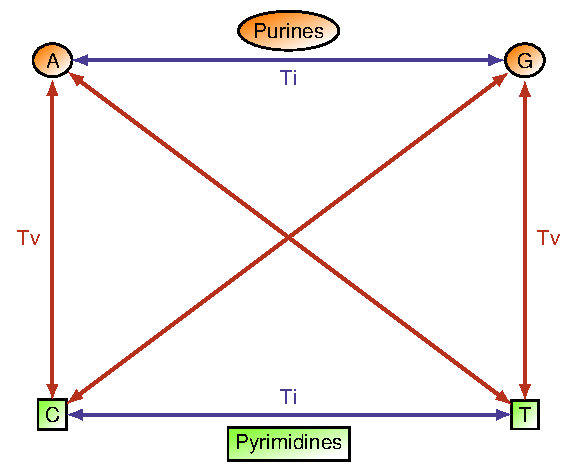
\includegraphics[width=0.95\textwidth]{TiTv_diagram.pdf}}
\end{minipage}\hspace{-0.3cm}
\begin{minipage}[c]{0.35\textwidth}
    \captionof{figure}{Purines (A and G) and pyrimidines (C and T) are shown. Transitions occur when a mutation involves purine-to-purine or pyrimidine-to-pyrimidine insertion. Transversions occur when a purine-to-pyrimidine or pyrimidine-to-purine insertion happens, which is a more extreme case. There are visibly more possibilities for transversions to occur than there are transitions, but there are about twice as many transitions in real data.}\label{fig:TiTv_diagram}
\end{minipage}

\bigskip

This information is always given in a particular data set. Let $\gamma_0$, $\gamma_1$, and $\gamma_2$ denote the probabilities of PuPu, PuPy, and PyPy, respectively, for the $p$ loci of data matrix $X$. In real data, there are approximately twice as many transitions as there are transversions. That is, the probability of a transition $\text{P}(\text{Ti})$ is approximately twice the probability of transversion $\text{P}(\text{Tv})$. It is likely that any particular data set will not satisfy this criterion exactly. In this general case, we have $\text{P}(\text{Ti})$ being equal to some multiple $\eta$ times $\text{P}(\text{Tv})$. In order to enforce this general constraint in simulated data, we define the following set of equalities
%
\begin{alignat}{2}\label{eq:TiTv_constraints1}
\gamma_0 + \gamma_1 + \gamma_2 &= 1, \\ \label{eq:TiTv_constraints2}
\text{P}(\text{Ti}) - \eta \text{P}(\text{Tv}) &= 0.
\end{alignat}

Using this PuPu, PuPy, and PyPy encoding, the probability of a transversion occuring at any fixed locus $a$ is given by the following
%
\begin{equation}\label{eq:prob_Tv}
\begin{aligned}
\text{P}(\text{Tv}) &= \gamma_1.
\end{aligned}
\end{equation}

Using the constraints given by Eqs.~\ref{eq:TiTv_constraints1} and \ref{eq:TiTv_constraints2}, the probability of a transition occuring at locus $a$ is computed as follows
%
\begin{equation}\label{eq:prob_Ti}
\begin{aligned}
\text{P}(\text{Ti}) &= \gamma_0 + \gamma_2.
\end{aligned}
\end{equation}

Also based on the constraints given by Eqs.~\ref{eq:TiTv_constraints1} and \ref{eq:TiTv_constraints2}, it is clear that we have $\text{P}(\text{Tv}) = \frac{1}{\eta + 1}$ and $\text{P}(\text{Ti}) = \frac{\eta}{\eta + 1}$. Without loss of generality, we then sample 
%
\begin{equation}\label{eq:gamma0}
\gamma_0 \sim \mathcal{U}\left(\varepsilon,\frac{\eta}{\eta + 1} - \varepsilon\right),
\end{equation}
where $\varepsilon$ is some small positive real number.

Then it immediately follows that we have 
%
\begin{equation}\label{eq:gamma2}
\gamma_2 = \frac{\eta}{\eta + 1} - \gamma_0.
\end{equation}

However, we can derive the mean and variance of the distance distribution induced by the TiTv metric without specifying any relationship between $\gamma_0$, $\gamma_1$, and $\gamma_2$. We proceed by computing $\text{P}\left[d^\text{TiTv}_{ij}(a) = k\right]$ for each $k \in \mathcal{D} = \bigl\{0,\frac{1}{4},\frac{1}{2},\frac{3}{4},1\bigr\}$. Let $y$ represent a random sample of size $p$ from $\{0,1,2\}$, where 
%
\begin{equation}\label{eq:yvec}
y_a = \begin{cases}
0 & \text{if locus } a \text{ is PuPu}, \\
1 & \text{if locus } a \text{ is PuPy}, \\
2 & \text{if locus } a \text{ is PyPy}.
\end{cases}
\end{equation}

We derive $\text{P}\left[d^\text{TiTv}_{ij}(a) = 0\right]$ as follows
%
\begin{equation}\label{eq:prob_TiTv_0}
\begin{aligned}
\text{P}\left[d^\text{TiTv}_{ij}(a) = 0\right] &= \text{P}\left[y_a = 0, X_{ia} = X_{ja}\right] \\
&+ \text{P}\left[y_a = 1, X_{ia} = X_{ja}\right] \\
&+ \text{P}\left[y_a = 2, X_{ia} = X_{ja}\right] \\
&= \gamma_0 \left[(1 - f_a)^2 + 4 f_a (1 - f_a) + f^2_a\right] \\
&+ \gamma_1 \left[(1 - f_a)^2 + 4 f_a (1 - f_a) + f^2_a\right] \\
&+ \gamma_2 \left[(1 - f_a)^2 + 4 f_a (1 - f_a) + f^2_a\right] \\
&= (\gamma_0 + \gamma_1 + \gamma_2)\left[(1 - f_a)^2 + 4 f_a (1 - f_a) + f^2_a\right] \\
&= (1 - f_a)^2 + 4 f_a (1 - f_a) + f^2_a.
\end{aligned}
\end{equation}

We derive $\text{P}\left[d^\text{TiTv}_{ij}(a) = \frac{1}{4}\right]$ as follows
%
\begin{equation}\label{eq:prob_TiTv_0.25}
\begin{aligned}
\text{P}\left[d^\text{TiTv}_{ij}(a) = \frac{1}{4}\right] &= 2 \text{P}\left[y_a = 0, X_{ia} = 0, X_{ja} = 1\right] \\
&+ 2 \text{P}\left[y_a = 0, X_{ia} = 1, X_{ja} = 2\right] \\
&+ 2 \text{P}\left[y_a = 2, X_{ia} = 0, X_{ja} = 1\right] \\
&+ 2 \text{P}\left[y_a = 2, X_{ia} = 1, X_{ja} = 2\right] \\
&= 4 \gamma_0 (1 - f_a)^3 f_a + 4 \gamma_0 f^3_a (1 - f_a) + 4 \gamma_2 (1 - f_a)^3 f_a \\
&+ 4 \gamma_2 f^3_a (1 - f_a) \\
&= 4 \gamma_0 \left[(1 - f_a)^3 f_a + f^3_a (1 - f_a)\right] \\
&+ 4 \gamma_2 \left[(1 - f_a)^3 f_a + f^3_a (1 - f_a)\right] \\
&= 4(\gamma_0 + \gamma_2)\left[(1 - f_a)^3 f_a + f^3_a (1 - f_a)\right].
\end{aligned}
\end{equation}

We derive $\text{P}\left[d^\text{TiTv}_{ij}(a) = \frac{1}{2}\right]$ as follows
%
\begin{equation}\label{eq:prob_TiTv_0.5}
\begin{aligned}
\text{P}\left[d^\text{TiTv}_{ij}(a) = \frac{1}{2}\right] &= 2 \text{P}\left[y_a = 1, X_{ia} = 0, X_{ja} = 1\right] \\
&+ 2 \text{P}\left[y_a = 1, X_{ia} = 1, X_{ja} = 2\right] \\
&= 4 \gamma_1 (1 - f_a)^3 f_a + 4 \gamma_1 f^3_a (1 - f_a) \\
&= 4 \gamma_1 \left[(1 - f_a)^3 f_a + f^3_a (1 - f_a)\right].
\end{aligned}
\end{equation}

We derive $\text{P}\left[d^\text{TiTv}_{ij}(a) = \frac{3}{4}\right]$ as follows
%
\begin{equation}\label{eq:prob_TiTv_0.75}
\begin{aligned}
\text{P}\left[d^\text{TiTv}_{ij}(a) = \frac{3}{4}\right] &= 2 \text{P}\left[y_a = 0, X_{ia} = 0, X_{ja} = 2\right] \\
&+ 2 \text{P}\left[y_a = 2, X_{ia} = 0, X_{ja} = 2\right] \\
&= 2 \gamma_0 (1 - f_a)^2 f^2_a + 2 \gamma_2 (1 - f_a)^2 f^2_a \\
&= 2(\gamma_0 + \gamma_2)(1 - f_a)^2 f^2_a.
\end{aligned}
\end{equation}

We derive $\text{P}\left[d^\text{TiTv}_{ij}(a) = 1\right]$ as follows
%
\begin{equation}\label{eq:prob_TiTv_1}
\begin{aligned}
\text{P}\left[d^\text{TiTv}_{ij}(a) = 1\right] &= 2 \text{P}\left[y_a = 1, X_{ia} = 0, X_{ja} = 2\right] \\
&= 2 \gamma_1 (1 - f_a)^2 f^2_a.
\end{aligned}
\end{equation}

Using Eqs. \ref{eq:prob_TiTv_0} - \ref{eq:prob_TiTv_1}, we compute the expected TiTv distance between instances $i$ and $j$ as follows
%
\begin{equation}\label{eq:mu_DDistr_TiTv}
\begin{aligned}
\text{E}\left(D^\text{TiTv}_{ij}\right) &= \sum_{a \in \mathcal{A}} \left(\sum_{k \in \mathcal{D}} k \cdot \text{P}\left[d^\text{TiTv}_{ij}(a) = k\right]\right) \\
&= (\gamma_0 + \gamma_2 + 2\gamma_1) \sum_{a \in \mathcal{A}} \left[(1 - f_a)^3 f_a + f^3_a (1 - f_a)\right] \\
&+ \left[\frac{3}{2}(\gamma_0 + \gamma_2) + 2\gamma_1\right] \sum_{a \in \mathcal{A}} (1 - f_a)^2 f^2_a \\
&= (\gamma_0 + \gamma_2 + 2\gamma_1) \sum_{a \in \mathcal{A}} F(a) + \left[\frac{3}{2}(\gamma_0 + \gamma_2) + 2\gamma_1\right] \sum_{a \in \mathcal{A}} G(a),
\end{aligned}
\end{equation}
where $F(a) = (1 - f_a)^3 f_a + f^3_a (1 - f_a)$ and $G(a) = (1 - f_a)^2 f^2_a$.

The second moment about the origin for the TiTv distance is computed as follows
%
\begin{equation}\label{eq:mu2_DDistr_TiTv}
\begin{aligned}
\text{E}\left[\left(D^\text{TiTv}_{ij}\right)^2\right] &= \text{E}\left[\left(\sum_{a \in \mathcal{A}} d^\text{TiTv}_{ij}(a)\right)^2\right] \\
&= \text{E}\left[\sum_{a \in \mathcal{A}} \left(d^\text{TiTv}_{ij}(a)\right)^2\right] + 2 \text{E}\left[\sum_{r \in \mathcal{A}} \sum_{s \leq r - 1} d^\text{TiTv}_{ij}(r) \cdot d^\text{TiTv}_{ij}(s)\right] \\
&= \sum_{a \in \mathcal{A}} \left(\sum_{k \in \mathcal{D}} k^2 \cdot \text{P}\left[d^\text{TiTv}_{ij}(a) = k\right]\right) \\
&+ 2\sum_{a \in \mathcal{A}} \sum_{s \leq r - 1} \left(\sum_{k \in \mathcal{D}} k \cdot \text{P}\left[d^\text{TiTv}_{ij}(r) = k\right]\right) \cdot \left(\sum_{k \in \mathcal{D}} k \cdot \text{P}\left[d^\text{TiTv}_{ij}(s) = k\right]\right) \\
&= \left[\frac{1}{4}(\gamma_0 + \gamma_2) + \gamma_1\right] \sum_{a \in \mathcal{A}} F(a) + \left[\frac{9}{8}(\gamma_0 + \gamma_2) + 2\gamma_1\right] \sum_{a \in \mathcal{A}} G(a) \\
&+ 2 \sum_{r \in \mathcal{A}} \sum_{s \leq r - 1} \prod_{\lambda \in \{r,s\}} \left([\gamma_0 + \gamma_2 + 2\gamma_1] F(\lambda) + \left[\frac{3}{2}(\gamma_0 + \gamma_2) + 2\gamma_1\right] G(\lambda)\right),
\end{aligned}
\end{equation}
where $F(\lambda) = (1 - f_\lambda)^3 f_\lambda + f^3_\lambda (1 - f_\lambda)$ and $G(\lambda) = (1 - f_\lambda)^2 f^2_\lambda$.

Using the moments given by Eqs. \ref{eq:mu_DDistr_TiTv} and \ref{eq:mu2_DDistr_TiTv}, the variance is computed as follows
%
\begin{equation}\label{eq:var_DDistr_TiTv}
\begin{aligned}
\text{Var}\left(D^\text{TiTv}_{ij}\right) &= \text{E}\left[\left(D^\text{TiTv}_{ij}\right)^2\right] - \left[\text{E}\left(D^\text{TiTv}_{ij}\right)\right]^2 \\
&=\left[\frac{1}{4}(\gamma_0 + \gamma_2) + \gamma_1\right] \sum_{a \in \mathcal{A}} F(a) + \left[\frac{9}{8}(\gamma_0 + \gamma_2) + 2\gamma_1\right] \sum_{a \in \mathcal{A}} G(a) \\
&+ 2 \sum_{r \in \mathcal{A}} \sum_{s \leq r - 1} \prod_{\lambda \in \{r,s\}} \left([\gamma_0 + \gamma_2 + 2\gamma_1] F(\lambda) + \left[\frac{3}{2}(\gamma_0 + \gamma_2) + 2\gamma_1\right] G(\lambda)\right) \\
&- \left([\gamma_0 + \gamma_2 + 2\gamma_1] \sum_{a \in \mathcal{A}} F(a) + \left[\frac{3}{2}(\gamma_0 + \gamma_2) + 2\gamma_1\right] \sum_{a \in \mathcal{A}} G(a)\right)^2 \\
&=\left[\frac{1}{4}(\gamma_0 + \gamma_2) + \gamma_1\right] \sum_{a \in \mathcal{A}} F(a) + \left[\frac{9}{8}(\gamma_0 + \gamma_2) + 2\gamma_1\right] \sum_{a \in \mathcal{A}} G(a) \\
&- \sum_{a \in \mathcal{A}} \left([\gamma_0 + \gamma_2 + 2\gamma_1] F(a) + \left[\frac{3}{2}(\gamma_0 + \gamma_2) + 2\gamma_1\right] G(a)\right)^2,
\end{aligned}
\end{equation}
where $F(a) = (1 - f_a)^3 f_a + f^3_a (1 - f_a)$ and $G(a) = (1 - f_a)^2 f^2_a$.

With the mean and variance estimates given by Eqs. \ref{eq:mu_DDistr_TiTv} and \ref{eq:var_DDistr_TiTv}, the asymptotic TiTv distance distribution is given by the following
%
\begin{equation}\label{eq:DDistr_TiTv}
\begin{aligned}
D^\text{TiTv}_{ij} \overset{.}{\sim} \mathcal{N}\Biggl(& (\gamma_0 + \gamma_2 + 2\gamma_1) \sum_{a \in \mathcal{A}} F(a) + \left[\frac{3}{2}(\gamma_0 + \gamma_2) + 2\gamma_1\right] \sum_{a \in \mathcal{A}} G(a), \\
&\left[\frac{1}{4}(\gamma_0 + \gamma_2) + \gamma_1\right] \sum_{a \in \mathcal{A}} F(a) + \left[\frac{9}{8}(\gamma_0 + \gamma_2) + 2\gamma_1\right] \sum_{a \in \mathcal{A}} G(a) \\
&- \sum_{a \in \mathcal{A}} \left([\gamma_0 + \gamma_2 + 2\gamma_1] F(a) + \left[\frac{3}{2}(\gamma_0 + \gamma_2) + 2\gamma_1\right] G(a)\right)^2\Biggr),
\end{aligned}
\end{equation}
where $F(a) = (1 - f_a)^3 f_a + f^3_a (1 - f_a)$ and $G(a) = (1 - f_a)^2 f^2_a$.

The relationship between the average success probability $\bar{f}_a$ and the predicted TiTv pairwise distance given by Eq.~\ref{eq:mu_DDistr_TiTv} is shown in Fig.~\ref{fig:TiTv-vs-maf}. Given upper and lower bounds $l$ and $u$, respectively, of the success probability sampling interval, the average success probability (or average MAF) is computed as follows
%
\begin{equation}\label{eq:avg_maf}
\bar{f}_a = \frac{1}{2}(l + u).
\end{equation}

The maximum distance occurs at $\bar{f}_a=0.5$, which is the inflection point about which the minor allele changes at locus $a$. If few minor alleles are present ($\bar{f}_a \to 0$), the predicted TiTv distance approaches 0. The same is true after the minor allele switches ($\bar{f}_a \to 1$).

\bigskip

\begin{minipage}[c]{0.65\textwidth}\hspace{-0.6cm}
	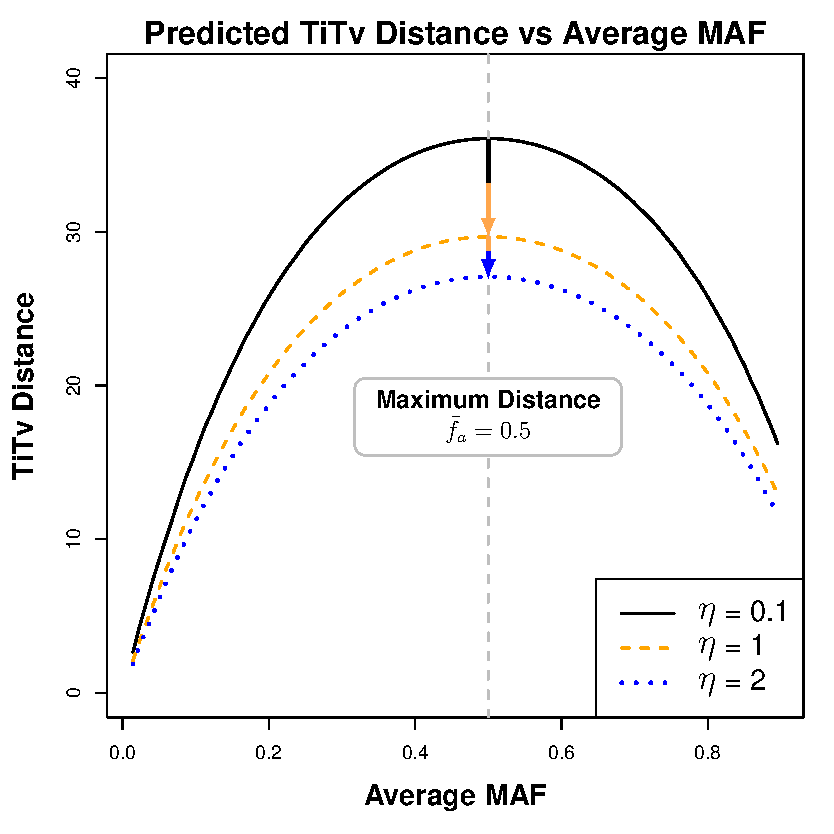
\includegraphics[width=0.98\textwidth]{TiTv_distance-vs-maf.pdf}
\end{minipage}\hspace{-0.8cm}
\begin{minipage}[c]{0.35\textwidth}
	\captionof{figure}{Predicted average TiTv distance as a function of average minor allele frequency $\bar{f}_a$ (see Eq.~\ref{eq:avg_maf}). Success probabilities $f_a$ were drawn from a sliding window interval from 0.01 to 0.9 in increments of about 0.009. With $\eta=0.1$, where $\eta$ is the Ti/Tv ratio given by Eq.~\ref{eq:TiTv_constraints1}, Tv is ten times more likely than Ti so the distance is large. Increasing to $\eta=1$, Tv and Ti are equally likely so the distance is moderate.  In line with real data for $\eta=2$, Tv is half as likely as Ti so the distance is relatively small.}\label{fig:TiTv-vs-maf}
\end{minipage}

\bigskip

%\subsection{Resting-State fMRI Distance Distribution}
\subsection{Time series correlation-based distance distribution}

For time series correlation-based data, we consider the case where there are $m$ correlation matrices $A^{(p \times p)}$. In particular, we are focusing on resting-state fMRI (rs-fMRI) data, which falls into this category. The derivations that follow, however, are relevant to all correlation-based data fitting the assumptions we have adopted. The features in rs-fMRI are commonly Regions of Interest (ROIs), which are collections of highly correlated and spatially proximal voxels \cite{lee2013}. These correlations are between different ROIs for a particular brain atlas \cite{dickie2017}. Because the features are the ROIs themselves, this leads us to the following metric
%
\begin{equation}\label{eq:diff_rs-fMRI}
d^\text{ROI}_{ij}(a) = \sum_{k \neq a}\bigl|A^{(i)}_{ka} - A^{(j)}_{ka}\bigr|.
\end{equation}
where $A^{(i)}_{ka}$ and $A^{(j)}_{ka}$ are the correlations between ROI $a$ and ROI $k$ for instances $i$ and $j$, respectively. In order for comparisons between different correlations to be possible, we first perform a Fisher r-to-z transform on the correlations. We then load all of the transformed correlations into a $p(p-1) \times m$ matrix $X$ (see Fig.~\ref{fig:rs-fMRI_matrix}).

\bigskip

\begin{minipage}[c]{0.7\textwidth}\hspace{-0.6cm}
	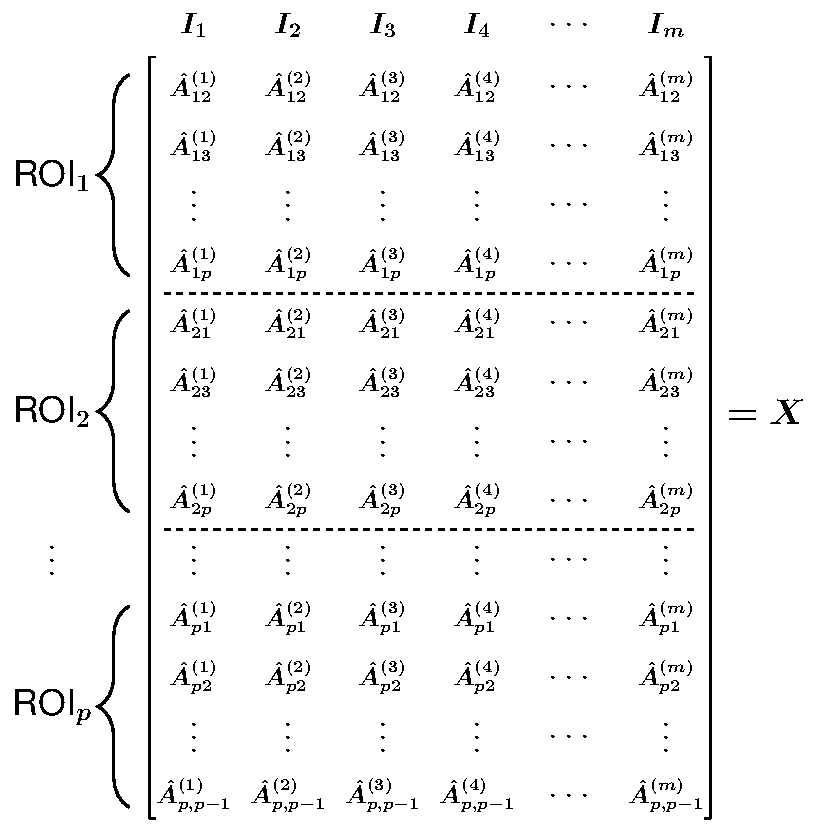
\includegraphics[width=0.95\textwidth]{rs_fmri_all_instance_matrix.pdf}
\end{minipage}\hspace{-0.8cm}
\begin{minipage}[c]{0.3\textwidth}
	\captionof{figure}{Resting-state fMRI transformed subject correlation matrices. Each column corresponds to an instance (or subject) $I_j$ and each column corresponds to an ROI (or feature). The notation $\hat{A}^{(j)}_{ka}$ represents the r-to-z transformed correlation between ROIs $a$ and $k \neq a$ for instance $j$.}\label{fig:rs-fMRI_matrix}
\end{minipage}

\bigskip

%
%\begin{equation}\label{eq:rs-fMRI_matrix}
%X = \left[
%\begin{array}{c c c c c}
%\hat{A}^{(1)}_{12} & \hat{A}^{(2)}_{12} & \hat{A}^{(3)}_{12} & \dots & \hat{A}^{(m)}_{12} \\
%\hat{A}^{(1)}_{13} & \hat{A}^{(2)}_{13} & \hat{A}^{(3)}_{13} & \dots & \hat{A}^{(m)}_{13} \\
%\hat{A}^{(1)}_{14} & \hat{A}^{(2)}_{14} & \hat{A}^{(3)}_{14} & \dots & \hat{A}^{(m)}_{14} \\
%\vdots & \vdots & \vdots & \ddots & \vdots \\
%\hat{A}^{(1)}_{1p} & \hat{A}^{(2)}_{1p} & \hat{A}^{(3)}_{1p} & \dots & \hat{A}^{(m)}_{1p} \\
%\hat{A}^{(1)}_{21} & \hat{A}^{(2)}_{21} & \hat{A}^{(3)}_{21} & \dots & \hat{A}^{(m)}_{21} \\
%\hat{A}^{(1)}_{23} & \hat{A}^{(2)}_{23} & \hat{A}^{(3)}_{23} & \dots & \hat{A}^{(m)}_{23} \\
%\hat{A}^{(1)}_{24} & \hat{A}^{(2)}_{24} & \hat{A}^{(3)}_{24} & \dots & \hat{A}^{(m)}_{24} \\
%\vdots & \vdots & \vdots & \ddots & \vdots \\
%\hat{A}^{(1)}_{2p} & \hat{A}^{(2)}_{2p} & \hat{A}^{(3)}_{2p} & \dots & \hat{A}^{(m)}_{2p} \\
%\vdots & \vdots & \vdots & \ddots & \vdots \\
%\hat{A}^{(1)}_{p1} & \hat{A}^{(2)}_{p1} & \hat{A}^{(3)}_{p1} & \dots & \hat{A}^{(m)}_{p1} \\
%\hat{A}^{(1)}_{p2} & \hat{A}^{(2)}_{p2} & \hat{A}^{(3)}_{p2} & \dots & \hat{A}^{(m)}_{p2} \\
%\hat{A}^{(1)}_{p3} & \hat{A}^{(2)}_{p3} & \hat{A}^{(3)}_{p3} & \dots & \hat{A}^{(m)}_{p3} \\
%\vdots & \vdots & \vdots & \ddots & \vdots \\
%\hat{A}^{(1)}_{p,(p-1)} & \hat{A}^{(2)}_{p,(p-1)} & \hat{A}^{(3)}_{p,(p-1)} & \dots & \hat{A}^{(m)}_{p,(p-1)}
%\end{array}
%\right],
%\end{equation}

We further transform the data matrix $X$ by standardizing so that each of the $m$ columns has zero mean and unit variance. Therefore, the data in matrix $X$ are standard normal. Recall from Eqs. \ref{eq:normalManMean} and \ref{eq:normalManVar}, that the mean and variance of the Manhattan ($q=1$) distance distribution for standard normal data are $\frac{2p}{\sqrt{\pi}}$ and $\frac{2(\pi - 2)p}{\pi}$, respectively. This allows us to easily derive the expected pairwise distance between instances $i$ and $j$ in rs-fMRI data as follows
%
\begin{equation}\label{eq:mu_DDistr_rs-fMRI}
\begin{aligned}
\text{E}(D^\text{fMRI}_{ij}) &= \text{E}\left(\sum_{a \in \mathcal{A}} d^\text{ROI}_{ij}(a)\right) \\
&= \text{E}\left(\sum_{a \in \mathcal{A}} \sum_{k \neq a} \bigl|\hat{A}^{(i)}_{ak} - \hat{A}^{(j)}_{ak}\bigr|\right) \\
&= \sum_{a \in \mathcal{A}} \sum_{k \neq a} \text{E}\left(\bigl|\hat{A}^{(i)}_{ak} - \hat{A}^{(j)}_{ak}\bigr|\right) \\
&= \sum_{a \in \mathcal{A}} \sum_{k \neq a} \frac{2}{\sqrt{\pi}} \\
&= \frac{2p(p-1)}{\sqrt{\pi}}.
\end{aligned}
\end{equation}

Due to the dependencies that exist between terms in the double sum when computing the rs-fMRI distance, linearity no longer applies to the variance operator. We proceed by writing the form of the variance as follows
%
\begin{equation}\label{eq:var_DDistr_rs-fMRI}
\begin{aligned}
\text{Var}(D^\text{fMRI}_{ij}) &= \text{Var}\left(\sum_{a \in \mathcal{A}} \sum_{k \neq a} \bigl|\hat{A}^{(i)}_{ak} - \hat{A}^{(j)}_{ak}\bigr|\right) \\
&= \sum_{a = 1}^{p-1} \text{Var}\left(\sum_{k=a+1}^{p} 2\bigl|\hat{A}^{(i)}_{ak} - \hat{A}^{(j)}_{ak}\bigr|\right) \\
&+ 2\sum_{a = 1}^{p-1} \sum_{r=a+1}^{p-1} \text{Cov}\left(\sum_{k=a+1}^{p} 2\bigl|\hat{A}^{(i)}_{ak} - \hat{A}^{(j)}_{ak}\bigr|, \sum_{s=r+1}^{p} 2\bigl|\hat{A}^{(i)}_{rs} - \hat{A}^{(j)}_{rs}\bigr|\right) \\
&= \sum_{a=1}^{p-1} \sum_{k=a+1}^{p} \text{Var}\left(2\bigl|\hat{A}^{(i)}_{ak} - \hat{A}^{(j)}_{ak}\bigr|\right) \\
&+ 2\sum_{a = 1}^{p-1} \sum_{r=a+1}^{p-1} \text{Cov}\left(\sum_{k=a+1}^{p} 2\bigl|\hat{A}^{(i)}_{ak} - \hat{A}^{(j)}_{ak}\bigr|, \sum_{s=r+1}^{p} 2\bigl|\hat{A}^{(i)}_{rs} - \hat{A}^{(j)}_{rs}\bigr|\right) \\
&= \sum_{a = 1}^{p-1} \sum_{k=a+1}^{p-1}\frac{4(\pi-2)}{\pi} \\
&+ 2\sum_{a = 1}^{p-1} \sum_{r=a+1}^{p-1} \text{Cov}\left(\sum_{k=a+1}^{p} 2\bigl|\hat{A}^{(i)}_{ak} - \hat{A}^{(j)}_{ak}\bigr|, \sum_{s=r+1}^{p} 2\bigl|\hat{A}^{(i)}_{rs} - \hat{A}^{(j)}_{rs}\bigr|\right) \\
&= \frac{2p(\pi-2)(p-1)}{\pi} \\
&+ 2\sum_{a = 1}^{p-1} \sum_{r=a+1}^{p-1} \text{Cov}\left(\sum_{k=a+1}^{p} 2\bigl|\hat{A}^{(i)}_{ak} - \hat{A}^{(j)}_{ak}\bigr|, \sum_{s=r+1}^{p} 2\bigl|\hat{A}^{(i)}_{rs} - \hat{A}^{(j)}_{rs}\bigr|\right).
\end{aligned}
\end{equation}

In order to have a formula in terms of the number of ROIs $p$ only, we must estimate the double sum on the right-hand side of Eq. \ref{eq:var_DDistr_rs-fMRI}. Through simulation, it can be seen that the difference between the sample variance $S^2_{D_{ij}}$ and $\frac{2p(\pi-2)(p-1)}{\pi}$ has a quadratic relationship with $p$. More explicitly, we have the following relationship
%
\begin{equation}\label{eq:estimate_cov}
S^2_{D^\text{fMRI}_{ij}} - \frac{2p(\pi-2)(p-1)}{\pi} = \beta_1 p^2 + \beta_0 p.
\end{equation}

The coefficient estimates found through least squares fitting are $\beta_0 = - \beta_1 \approx 0.08$. These estimates allow one to infer a functional form for the double sum in the right-hand side of Eq. \ref{eq:var_DDistr_rs-fMRI} that is actually proportional to $\frac{2p(\pi-2)(p-1)}{\pi}$. That is, we have the following formula for approximating the double sum
%
\begin{equation}\label{eq:estimate_cov_form}
2\sum_{a = 1}^{p-1} \sum_{r=a+1}^{p-1} \text{Cov}\left(\sum_{k=a+1}^{p} 2\bigl|\hat{A}^{(i)}_{ak} - \hat{A}^{(j)}_{ak}\bigr|, \sum_{s=r+1}^{p} 2\bigl|\hat{A}^{(i)}_{rs} - \hat{A}^{(j)}_{rs}\bigr|\right) = \frac{p(\pi - 2)(p - 1)}{4\pi}.
\end{equation}

Therefore, the variance of the rs-fMRI distances is approximated well by the following
%
\begin{equation}\label{eq:var_DDistr_rs-fMRI2}
\text{Var}(D^\text{fMRI}_{ij}) = \frac{9p(\pi - 2)(p-1)}{4\pi}.
\end{equation}

With the mean and variance estimates given by Eqs. \ref{eq:mu_DDistr_rs-fMRI} and \ref{eq:var_DDistr_rs-fMRI2}, we have the following asymptotic distribution for rs-fMRI distances
%
\begin{equation}\label{eq:DDistr_rs-fMRI}
D^\text{fMRI}_{ij} \overset{.}{\sim} \mathcal{N}\left(\frac{2p(p-1)}{\sqrt{\pi}}, \frac{9p(\pi - 2)(p-1)}{4\pi}\right).
\end{equation}

Consider the max-min normalized rs-fMRI distance given by the following equation
%
\begin{equation}\label{eq:max-min_diff_rs-fMRI}
D^\text{fMRI*}_{ij} = \sum_{a \in \mathcal{A}} \sum_{k \neq a} \frac{\bigl|A^{(i)}_{ak} - A^{(j)}_{ak}\bigr|}{\max(a) - \min(a)}.
\end{equation}

Assuming that the data $X$ has been r-to-z transformed and standardized, we can easily compute the expected attribute range and variance of the attribute range. The expected maximum of a given attribute in data matrix $X$ is estimated by the following
%
\begin{equation}\label{eq:mean_max_rs-fMRI}
\text{E}\left(X^\text{max}_a - X^\text{min}_a\right) = 2\mu^{(1)}_\text{max}(m,p) = 2 \left[\frac{\text{log}(\text{log}(2))}{\Phi^{-1}\left(\frac{1}{m(p-1)}\right)} - \Phi^{-1}\left(\frac{1}{m(p-1)}\right)\right].
\end{equation}

The variance can be esimated with the following
%
\begin{equation}\label{eq:var_max_rs-fMRI}
\text{Var}\left(X^\text{max}_a - X^\text{min}_a\right) = \frac{\pi^2}{6\text{log}[m(p-1)]}.
\end{equation}

Let $\mu_{D^\text{fMRI}_{ij}}$ and $\sigma^2_{D^\text{fMRI}_{ij}}$ denote the mean and variance of the rs-fMRI distance distribution given by Eqs. \ref{eq:mu_DDistr_rs-fMRI} and \ref{eq:var_DDistr_rs-fMRI2}. Using the formulas for the mean and variance of the max-min normalized distance distribution given in Eq. \ref{eq:max-min_DDistr_normal}, we have the following asymptotic distribution for the max-min normalized rs-fMRI distances
%
\begin{equation}\label{eq:max-min_DDistr_normal_rs-fMRI}
D^\text{fMRI*}_{ij} \overset{.}{\sim} \mathcal{N}\left(\frac{\mu_{D^\text{fMRI}_{ij}}}{2\mu^{(1)}_\text{max}(m,p)}, \frac{6\sigma^2_{D^\text{fMRI}_{ij}}\text{log}[m(p-1)]}{\pi^2 + 24\left[\mu^{(1)}_\text{max}(m,p)\right]^2\text{log}[m(p-1)]}\right).
\end{equation}

\subsection{Normalized Manhattan \texorpdfstring{($q=1$)}{} for rs-fMRI}

Substituting the non-normalized mean given by Eq.~\ref{eq:mu_DDistr_rs-fMRI} into Eq.~\ref{eq:max-min_DDistr_normal_rs-fMRI} for the mean of the max-min normalized rs-fMRI metric, we have the following
%
\begin{equation}
\begin{aligned}
\text{E}\left(D^\text{fMRI*}_{ij}\right) &= \frac{\mu_{D^\text{fMRI}_{ij}}}{2\mu^{(1)}_\text{max}(m,p)} \\
&= \frac{p(p-1)}{\sqrt{\pi}\mu^{(1)}_\text{max}(m,p)},
\end{aligned}
\end{equation}
where $\mu^{(1)}_\text{max}(m,p)$ is given in Eq.~\ref{eq:mean_max_rs-fMRI}.

Similarly, the variance of $D^\text{fMRI*}_{ij}$ is given by
%
\begin{equation}
\begin{aligned}
\text{Var}\left(D^\text{fMRI*}_{ij}\right) &= \frac{6\sigma^2_{D^\text{fMRI}_{ij}}\text{log}[m(p-1)]}{\pi^2 + 24\left[\mu^{(1)}_\text{max}(m,p)\right]^2\text{log}[m(p-1)]} \\
&= \frac{27(\pi-2)\text{log}[m(p-1)](p-1)p}{2\pi\left(\pi^2 + 24\left[\mu^{(1)}_\text{max}(m,p)\right]^2\text{log}[m(p-1)]\right)},
\end{aligned}
\end{equation}
where $\mu^{(1)}_\text{max}(m,p)$ is given in Eq.~\ref{eq:mean_max_rs-fMRI}.

\section{Effects of correlation on distances}

All of the derivations presented in previous sections are for the cases where there is no correlation between instances or features. We assumed that any pair $(X_{ia},X_{ja})$ of data points for instances $i$ and $j$ and fixed feature $a$ were independent and identically distributed. This was done in order to determine asymptotic estimates in null data. That is, data with no main effects, interaction effects, or pairwise correlations between features. Within this highly simplified context, our asymptotic formulas for distributional moments are reliable. However, correlations do exist between features and instances in real data. There are a multitude of different statistical effects that impact distance distributional properties. Ultimately, divergence from normality is caused primarily by large magnitude pairwise correlation between features. Pairwise feature correlation can be the result of main effects, where features have different within-group means. On the other hand, there could be an underlying interaction network in which there are strong associations between features. If features are differentially correlated between phenotype groups, then interactions exist that change affect the distance distribution. In the following few sections, we consider particular cases of the $L_q$ metric for continuous and discrete data under the effects of pairwise feature correlation.

\subsection{Continuous data}

Consider $X^{(m \times p)}$ where $X_{ia} \sim \mathcal{N}(0,1)$ for all $i=1,2,\dots,m$ and $a=1,2,\dots,p$. Without loss of generality, we let $m=p=100$ and consider only the $L_2$ (Euclidean) metric. An illustration of the effects of correlation on distances with the given assumptions is shown in Fig.~\ref{fig:null-vs-corr-normal}. Each density curve shown in (\textcolor{blue}{blue}) is for a simulated distance matrix from data with some degree of pairwise correlation between features. Divergence from normality in distances is directly related to the average absolute pairwise correlation that exists in the simulated data. This measure is given by
%
\begin{equation}\label{eq:abs_corr}
\bar{r}_\text{abs} = \frac{2}{p(p-1)}\sum^{p-1}_{i=1} \sum_{j > i} r_{ij}
\end{equation}
%
where $r_{ij}$ is the correlation between features $i$ and $j$ across all instances $m$. The distance density curve (\textcolor{orange}{orange}) is representative of distances generated from random standard normal data with no added correlation. The mean and variance of this distribution are given by Eqs.~\ref{eq:normalEucMeanImproved} and \ref{eq:normalEucVar}, respectively, by substituting $p=100$ for the mean. From left-to-right and top-to-bottom, there is an increase in $\bar{r}_\text{abs}$. This very quickly introduces positive skewness and increased variability. The predicted and sample means, however, are approximately the same in each case due to linearity of the expectation operator. Because of the dependencies between features, the predicted variance of 1 obviously no longer holds. 

In order to introduce a controlled level of correlation between features, we created correlation matrices based on a random graph with specified connection probability, where features correspond to the vertices in each graph. We assigned high correlations to connected features from the random graph and low correlations to all non-connections. Using the upper-triangular cholesky factor $U$ for uncorrelated data matrix $X$, we computed the following product to create correlated data matrix $X^\text{corr}$
%
\begin{equation}\label{eq:cholesky}
X^\text{corr} = X U^\text{T}.
\end{equation}

The new data matrix given by Eq.~\ref{eq:cholesky} has approximately the same correlation structure as the randomly generated correlation matrix created from a random graph. The cholesky method is a standard approach in creating correlated data sets.

\begin{figure}[H]
	\centering
	\framebox{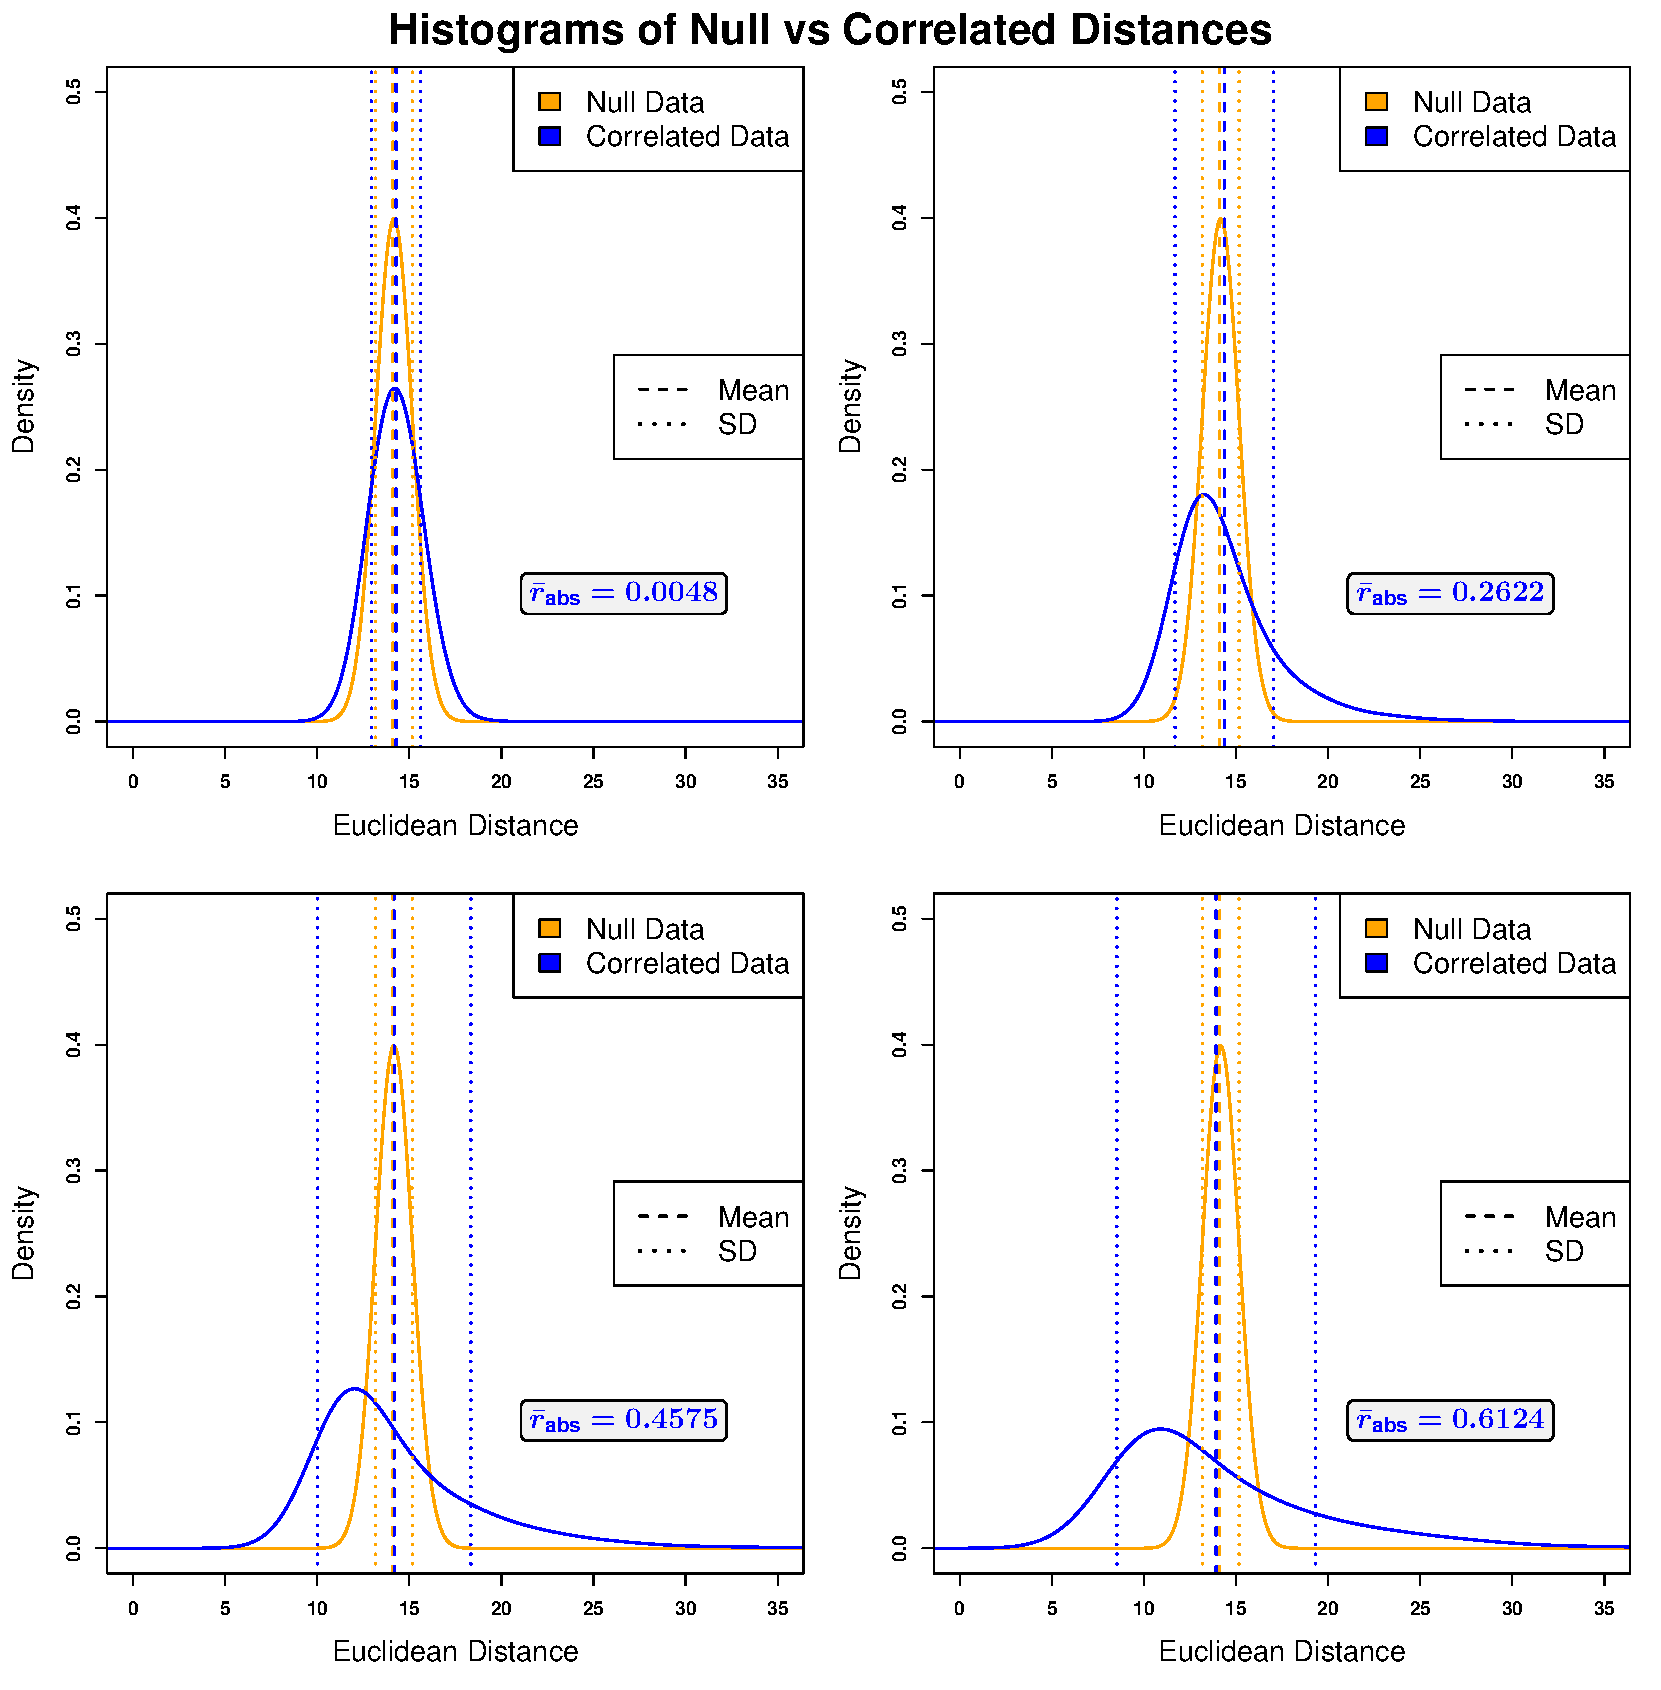
\includegraphics[width=0.98\textwidth]{null_vs_correlated_normal_euclidean_standard.pdf}}
	\caption{Density curves of distance distributions generated from correlated and uncorrelated data from standard normal distribution. Each plot has the theoretical density curve for the uncorrelated Euclidean distance distribution (\textcolor{orange}{orange}) and a density curve for Euclidean distances from correlated data (\textcolor{blue}{blue}) with some average magnitude pairwise correlation (\textcolor{blue}{$\bar{r}_\text{abs}$}) between features. (\textbf{Upper left}) With little correlation, distances begin to diverge from the predicted normal distribution. (\textbf{Upper Right}) Low to moderate correlation causes a large positive skew and increased variability in distances. (\textbf{Lower Left}) Moderate to high correlation increases skewness and variability in distances. (\textbf{Lower Right}) Extreme correlation produces maximal skewness and variability in distances. In each case, the null and correlated distance means are approximately the same.}\label{fig:null-vs-corr-normal}
\end{figure}

\subsection{GWAS data}

In analogy to the previous section, we explore the effects of pairwise feature correlation in the context of GWAS data. Without loss of generality, we let $m=p=100$ and consider the TiTv metric, which is given by combining Eqs.~\ref{eq:diff_TiTv} and \ref{eq:D} with $q=1$. To create correlated GWAS data, we first generated standard normal data with random correlation structure. We then applied the standard normal cumulative distribution function (CDF) to this correlated data, which was subsequently followed by the application of the inverse binomial CDF with random success probabilities for each feature (or SNP). The resulting GWAS data set is binomial with $n=2$ trials and has roughly the same correlation matrix as the correlated standard normal data.

\begin{figure}[H]
	\centering
	\framebox{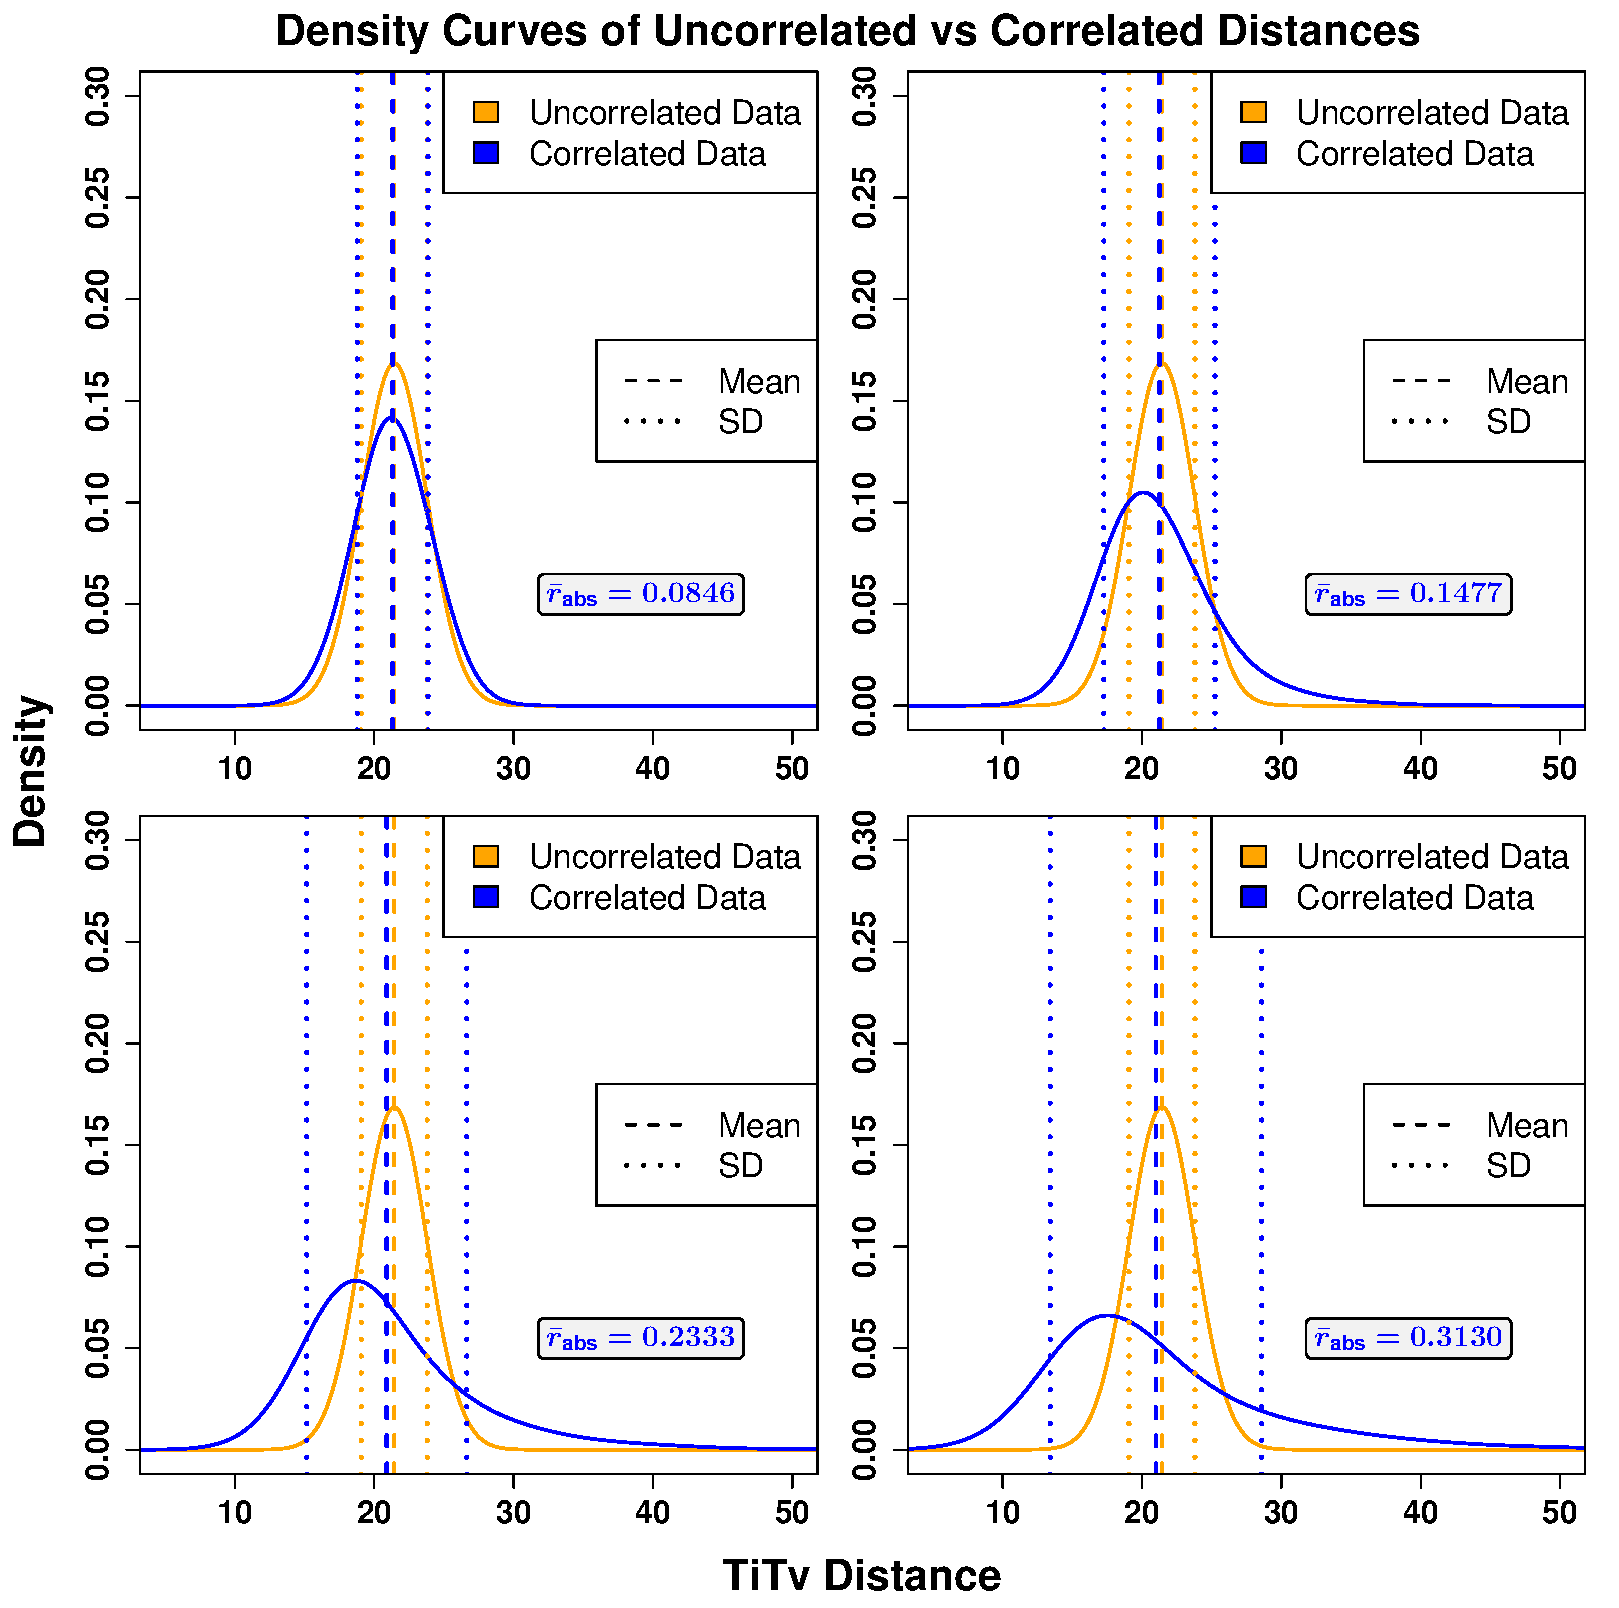
\includegraphics[width=0.98\textwidth]{null_vs_correlated_gwas_TiTv.pdf}}
	\caption{Density curves of distance distributions generated from correlated and uncorrelated data from a binomial distribution with $n=2$ trials and uniformly distributed success probabilities. Each plot has the theoretical density curve for the uncorrelated TiTv distance distribution (\textcolor{orange}{orange}) and a density curve for TiTv distances from correlated data (\textcolor{blue}{blue}) with some average magnitude pairwise correlation (\textcolor{blue}{$\bar{r}_\text{abs}$}) between features. (\textbf{Upper left}) With little correlation, distances begin to diverge from the predicted normal distribution. (\textbf{Upper Right}) Low to moderate correlation causes a large positive skew and increased variability in distances. (\textbf{Lower Left}) Moderate to high correlation increases skewness and variability in distances. (\textbf{Lower Right}) Extreme correlation produces maximal skewness and variability in distances. In each case, the null and correlated distance means are approximately the same.}\label{fig:null-vs-corr-titv}
\end{figure}

\subsection{Correlation-based data}

For our correlation data-based metric given by Eqs.~\ref{eq:diff_rs-fMRI} and \ref{eq:D} with $q=1$, we consider additional effects of correlation between features. Without loss of generality, we let $m=100$ and $p=30$. As in the previous subsections, an illustration of the effects of correlated features in this context is shown in Fig.~\ref{fig:null-vs-corr-rsfMRI}. Based on the correlated distance densities (\textcolor{blue}{blue}), it appears that correlation between features introduces positive skewness at lower values of $\bar{r}_\text{abs}$. We introduced correlation to the transformed data matrix given by Fig.~\ref{fig:rs-fMRI_matrix} with the cholesky method used previously.

\begin{figure}[H]
	\centering
	\framebox{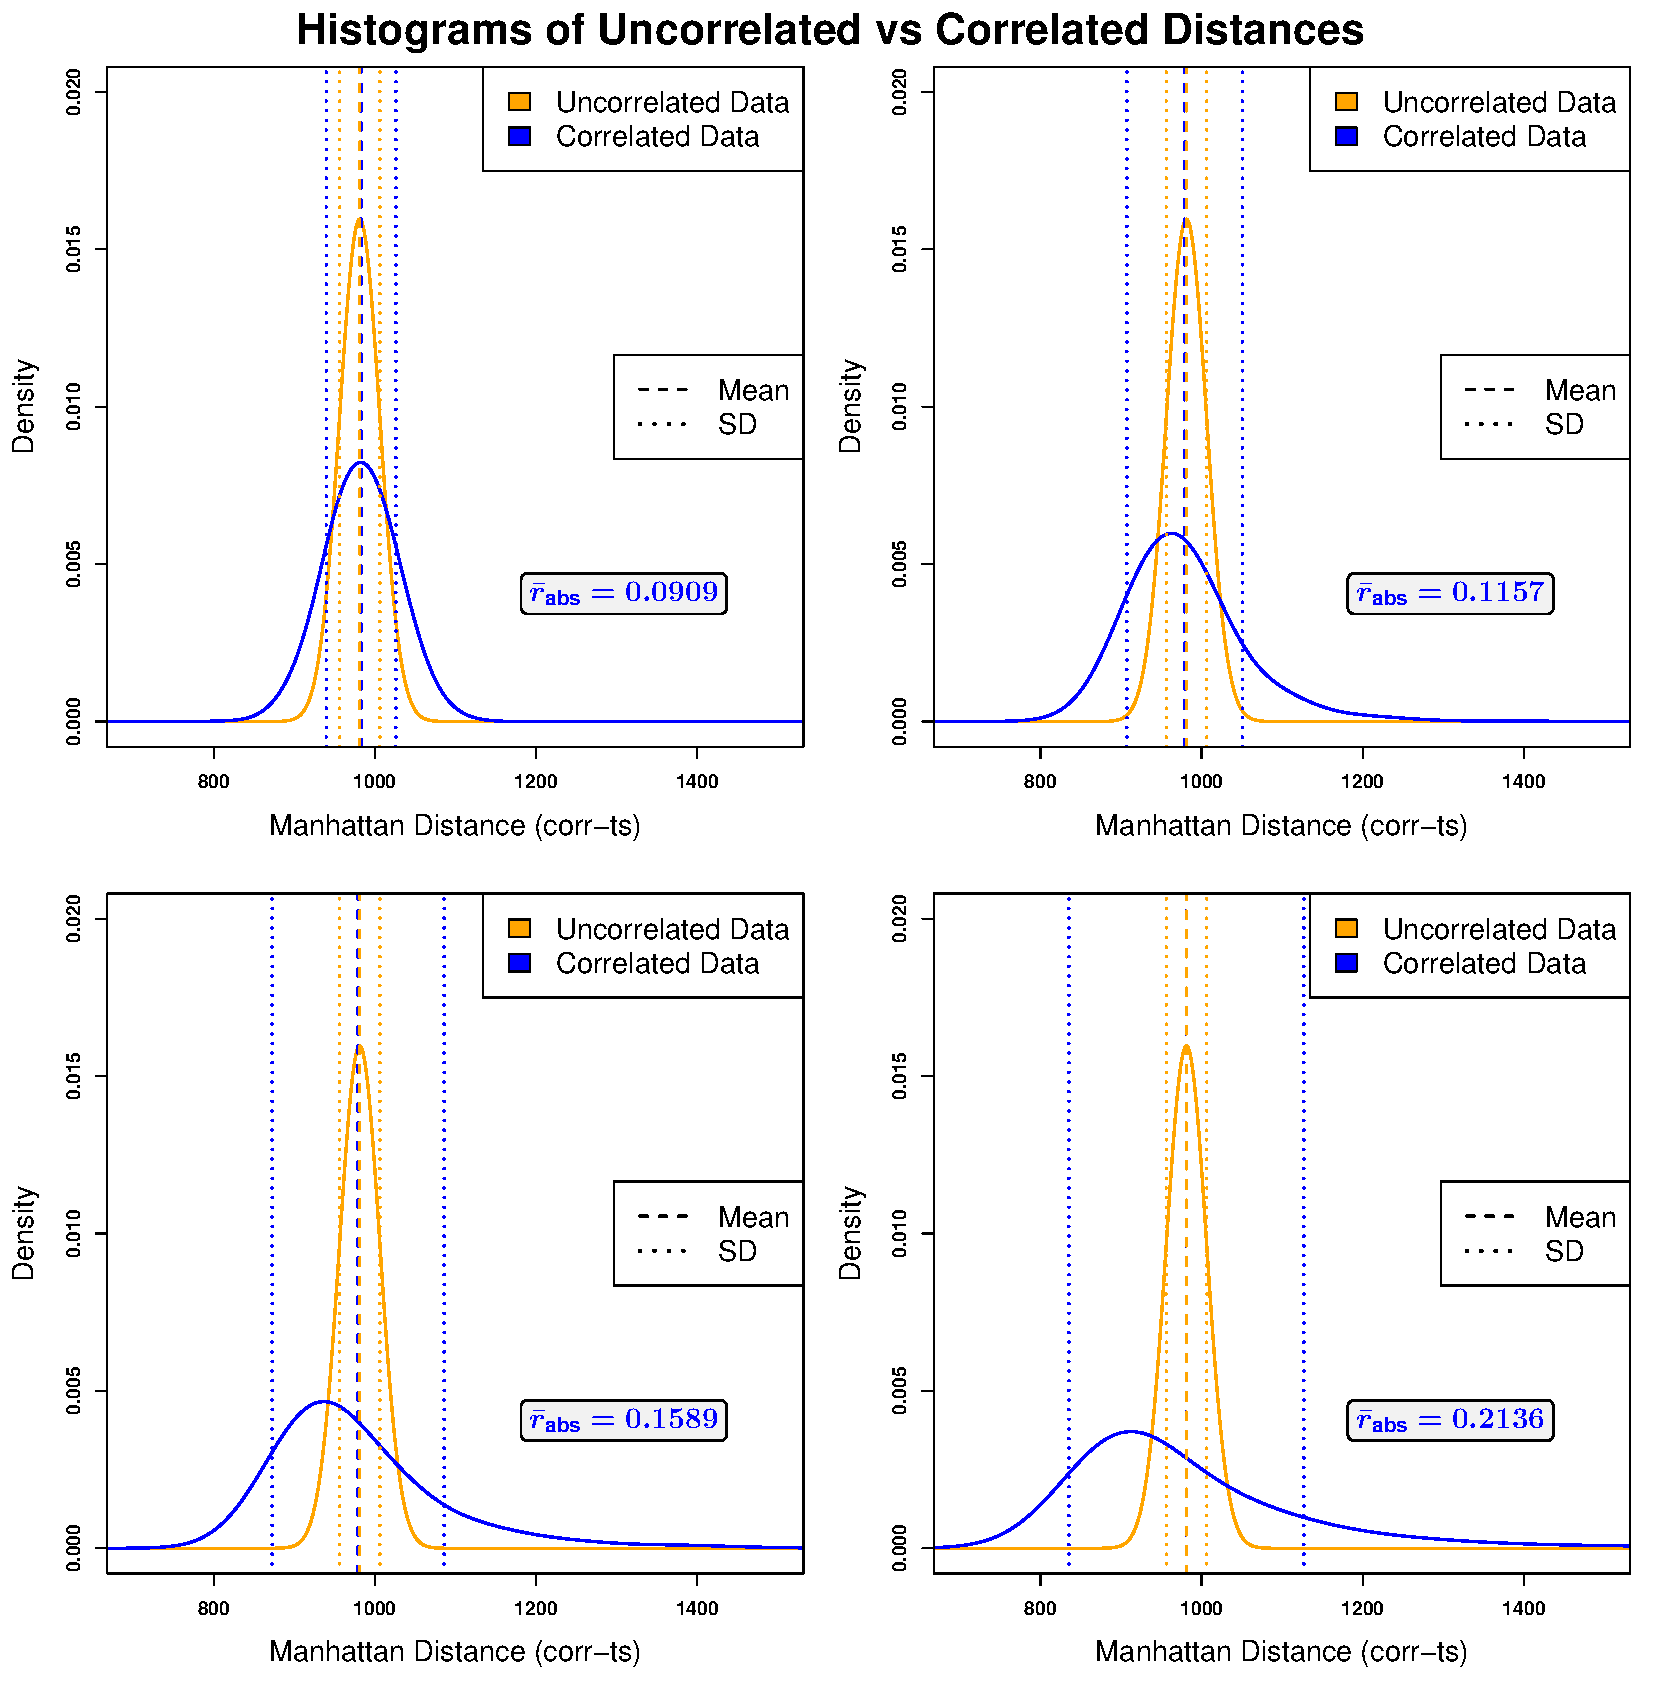
\includegraphics[width=0.98\textwidth]{null_vs_correlated_rsfMRI.pdf}}
	\caption{Density curves of distance distributions generated from correlated and uncorrelated transformed correlation data (see Fig.~\ref{fig:rs-fMRI_matrix}). Each plot has the theoretical density curve for the uncorrelated distance distribution (\textcolor{orange}{orange}) and a density curve for distances from correlated data (\textcolor{blue}{blue}) with some average magnitude pairwise correlation (\textcolor{blue}{$\bar{r}_\text{abs}$}) between features. (\textbf{Upper left}) With little correlation, distances begin to diverge from the predicted normal distribution. (\textbf{Upper Right}) Low to moderate correlation causes a large positive skew and increased variability in distances. (\textbf{Lower Left}) Moderate to high correlation increases skewness and variability in distances. (\textbf{Lower Right}) Extreme correlation produces maximal skewness and variability in distances. In each case, the null and correlated distance means are approximately the same.}\label{fig:null-vs-corr-rsfMRI}
\end{figure}

\begin{figure}[H]
	\centering
	\framebox{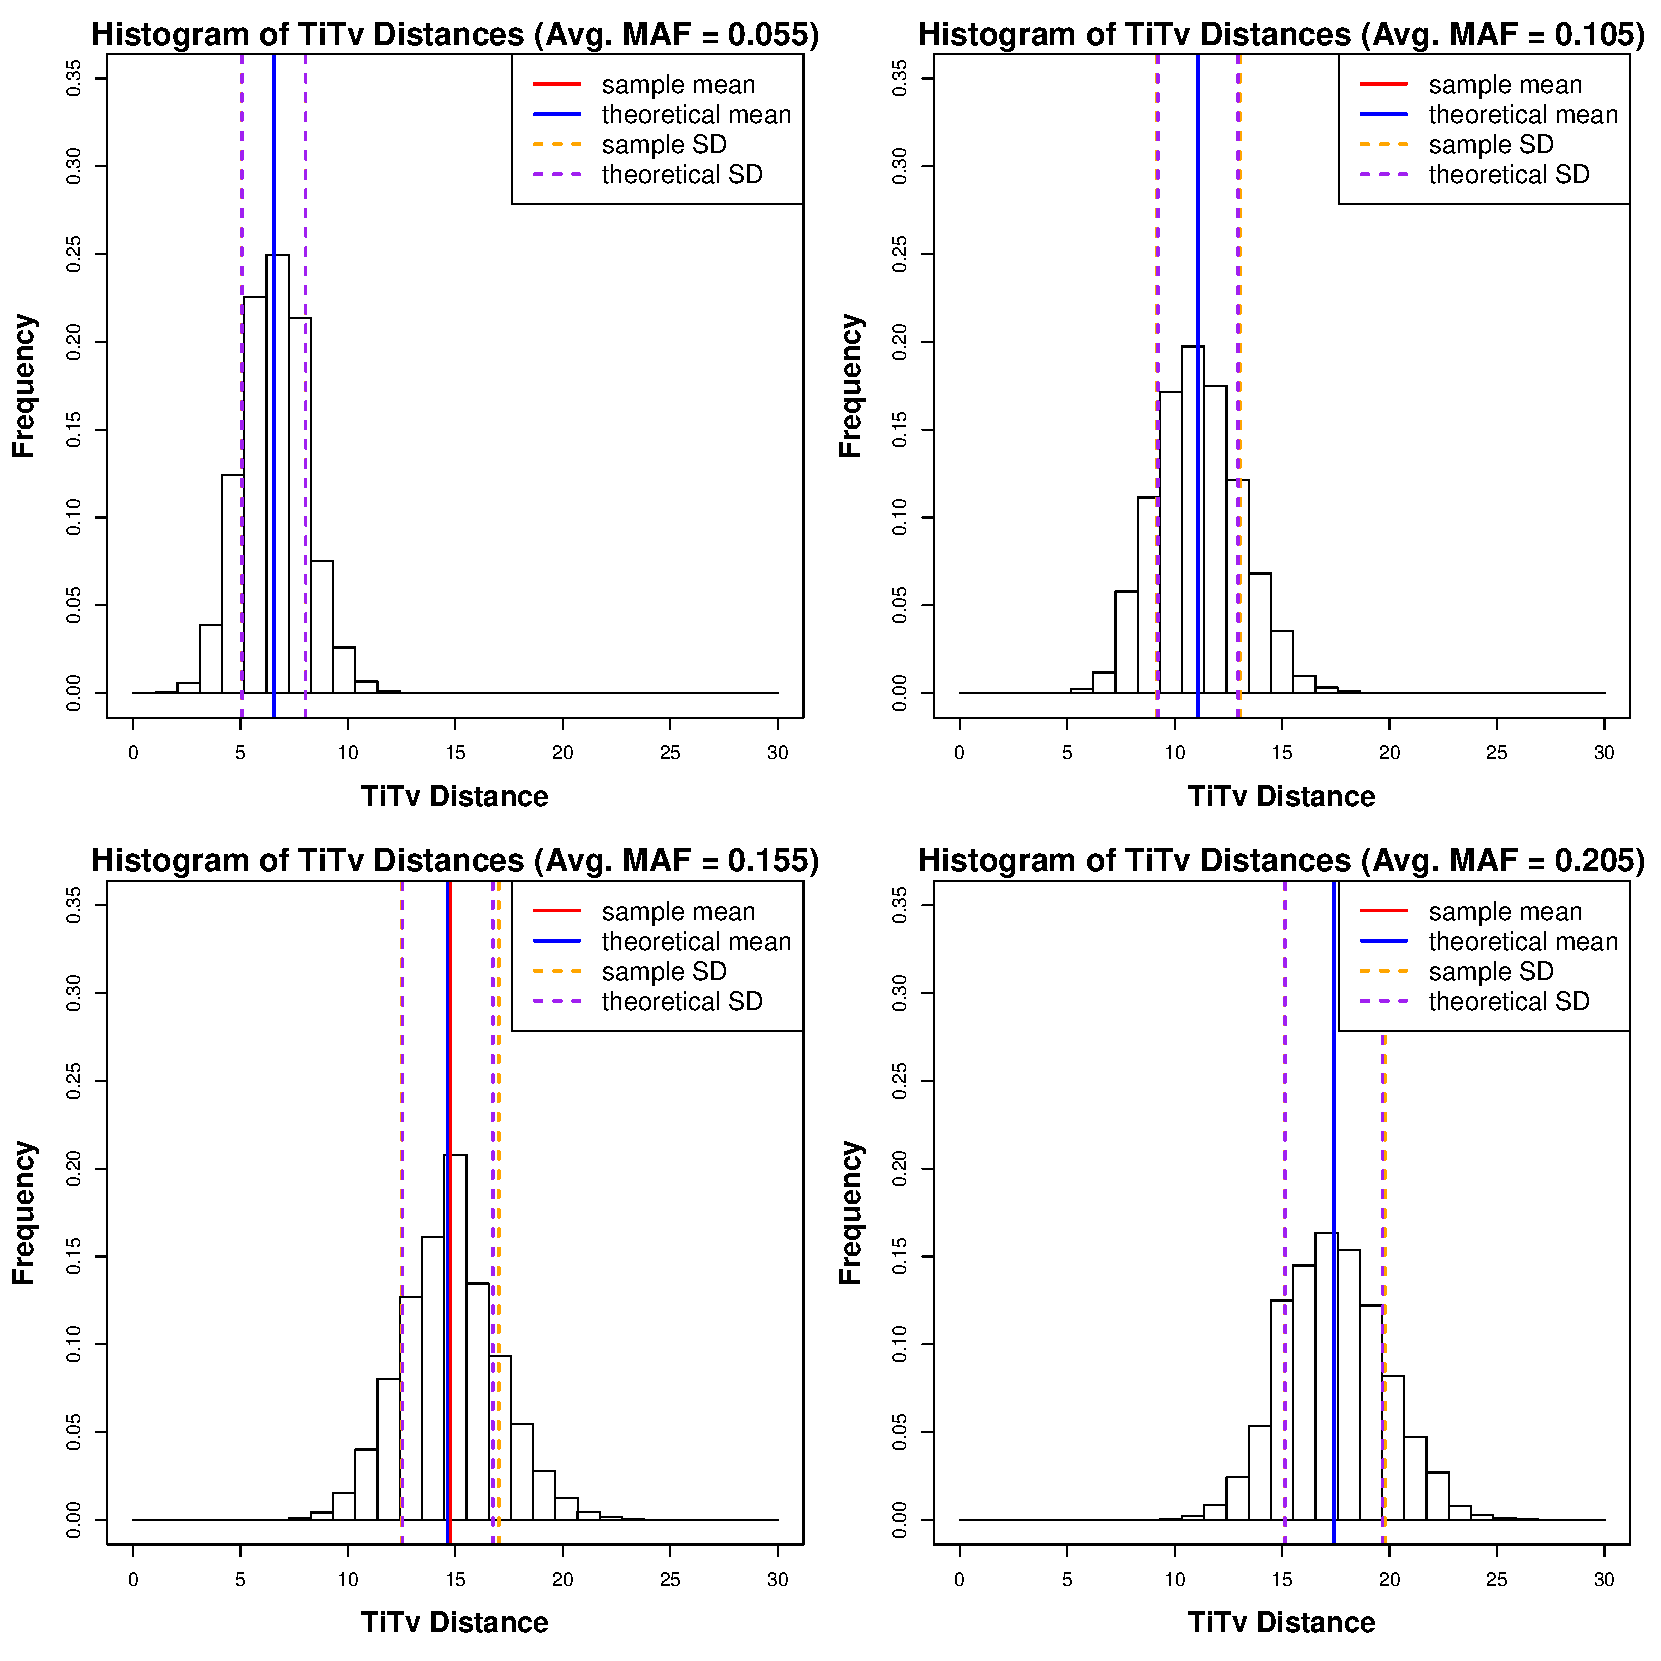
\includegraphics[width=0.98\textwidth]{TiTv_distance_histograms_MAFs.pdf}}
	\caption{Histograms of simulated TiTv distance distributions for different average MAFs. The Ti/Tv ratio was fixed to be 2 in all simulations. Average MAF is computed as the expected value of the uniform distribution from which minor allele success probabilities ($f_a$) are drawn. The upper bounds for each success probability uniform distribution are $\{0.1,0.2,0.3,0.4\}$, which are the maximum possible MAF for a given locus $a$. The corresponding lower bounds were $\{0.01,0.1,0.2,0.3\}$. Sample and predicted means, as well as standard deviations, are overlaid on each histogram. Each distance distribution comes from a simulated data set with $m=100$ instances and $p=100$ features.}\label{fig:TiTv_hist}
\end{figure}

\begin{figure}[H]
	\centering
	\framebox{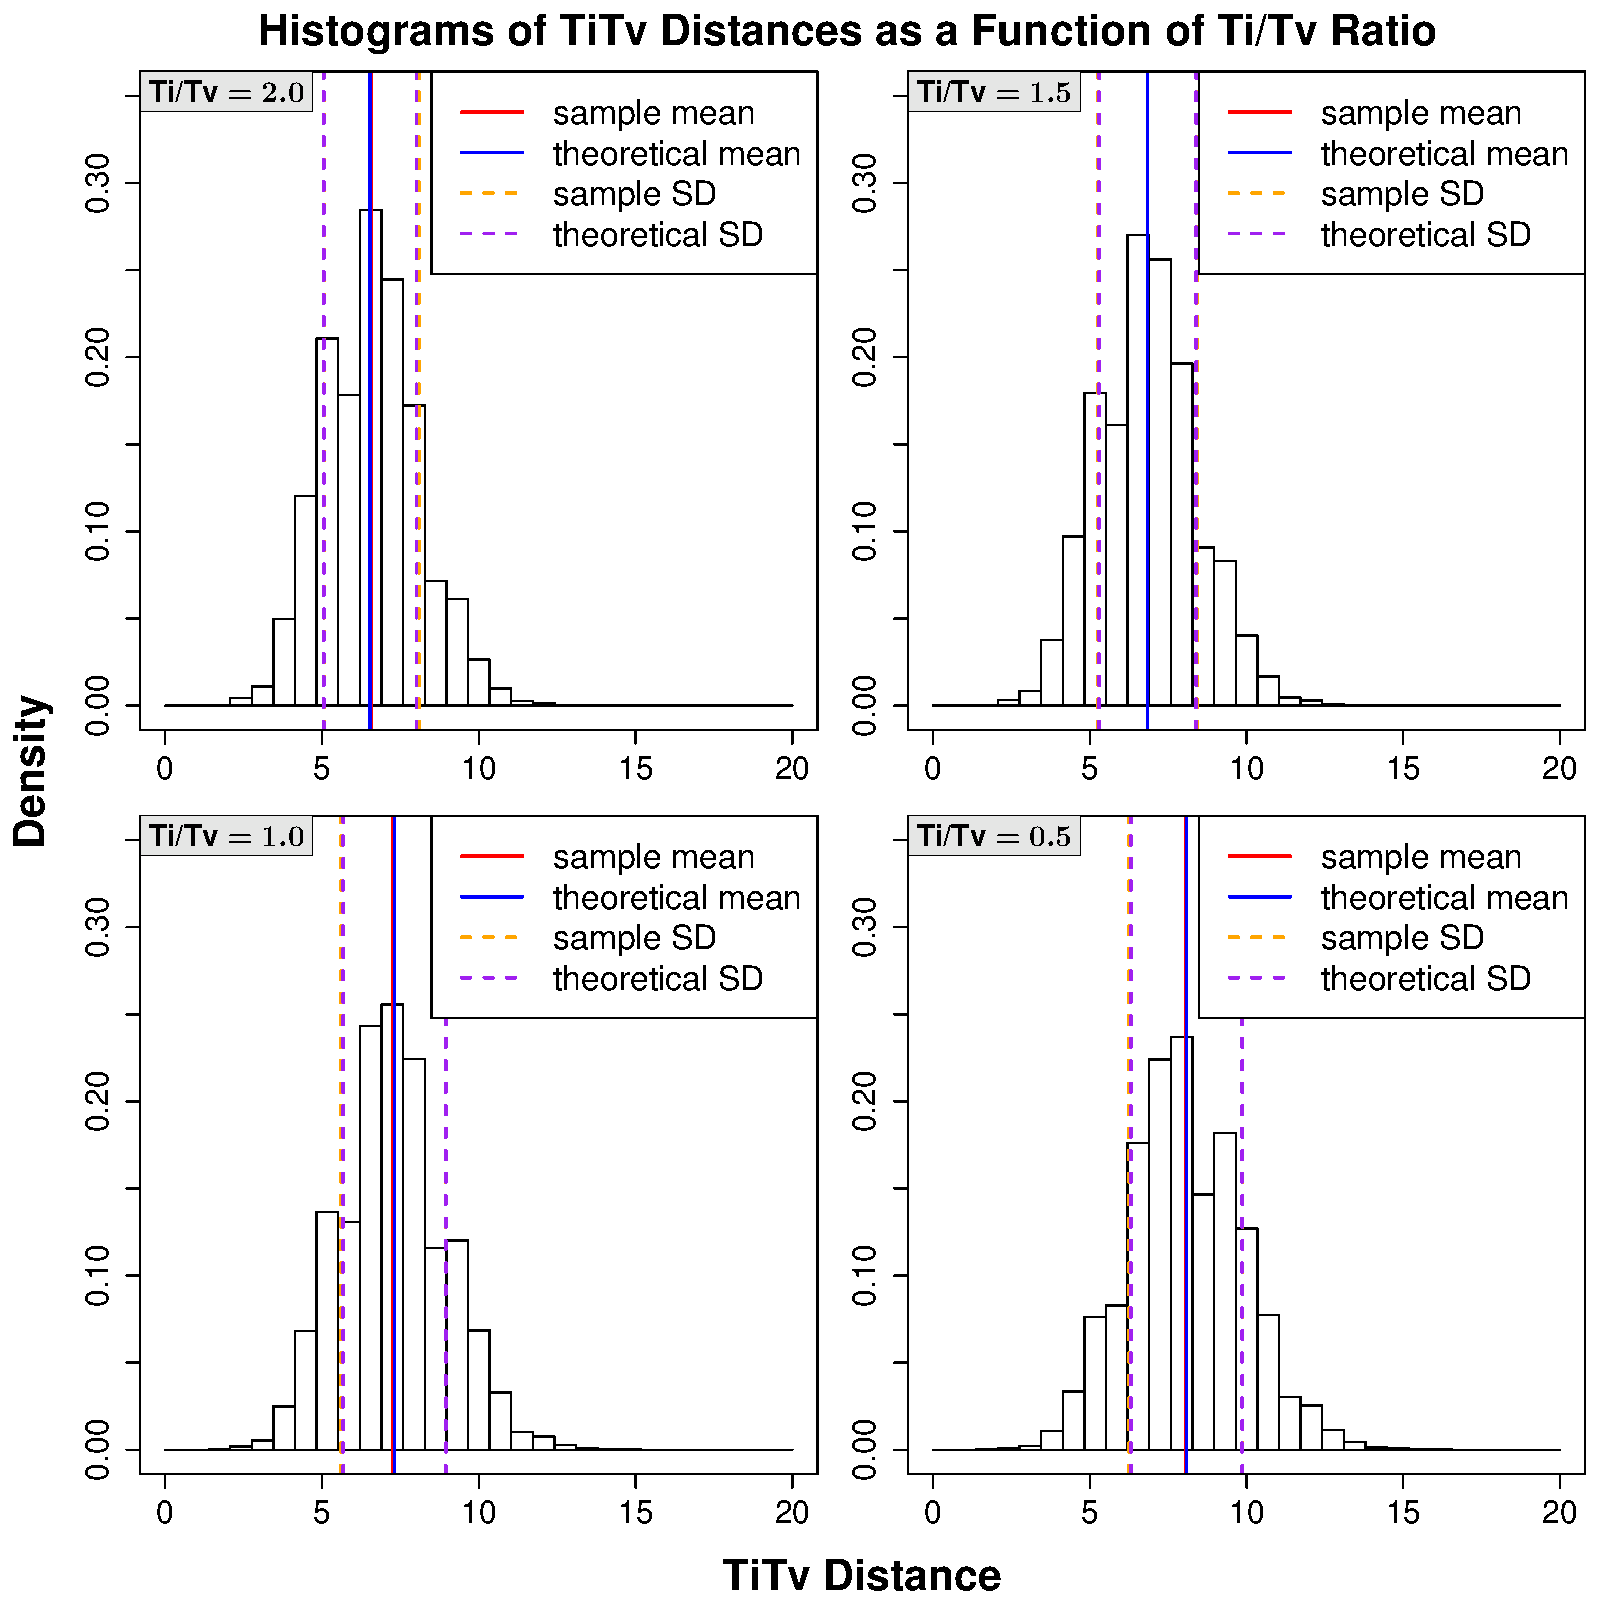
\includegraphics[width=0.98\textwidth]{TiTv_distance_histogram_TiTvs.pdf}}
	\caption{Histograms of simulated TiTv distance distributions for different Ti/Tv ratios. Average MAF was fixed to be 0.055. The Ti/Tv ratio was taken to be 2, 1.5, 1, and 0.5. The average distance increases as the Ti/Tv ratio decreases, which is intuitive because the TiTv distance is greater for transversions than transitions. Sample and predicted means, as well as standard deviations, are overlaid on each histogram. Each distance distribution comes from a simulated data set with $m=100$ instances and $p=100$ features.}\label{fig:TiTv_hist2}
\end{figure}

\section{Discussion}

\section{Conclusions}
% mean/variance tables

%\begin{table}[H]
%\caption{Summary of asymptotic distance distributions for common data types. Metrics with subscripts M and E represent Manhattan and Euclidean, respectively. Metrics with superscript $^*$ represent a deviation from the standard metric by attribute range normalization. The function $\Phi^{-1}(x)$ denotes the standard normal quantile function, where $x \in (0,1)$.}
%\label{tab:dist_distr_common}
%\centering
% trim=left botm right top
%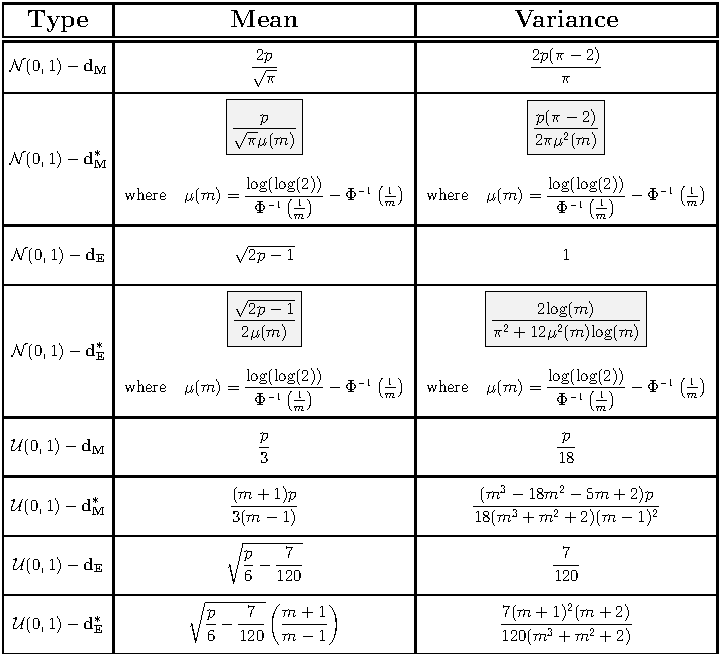
\includegraphics[width=\textwidth]{typical_data-metric_tab.pdf}
%\end{table}

%\begin{table}[H]
%\caption{Summary of asymptotic distance distributions for rs-fMRI and GWAS data. Metrics with superscript $^*$ represent a deviation from the standard metric by attribute range normalization. The function $\Phi^{-1}(x)$ denotes the standard normal quantile function, where $x \in (0,1)$.}
%\label{tab:dist_distr_bio}
%\centering
% trim=left botm right top
%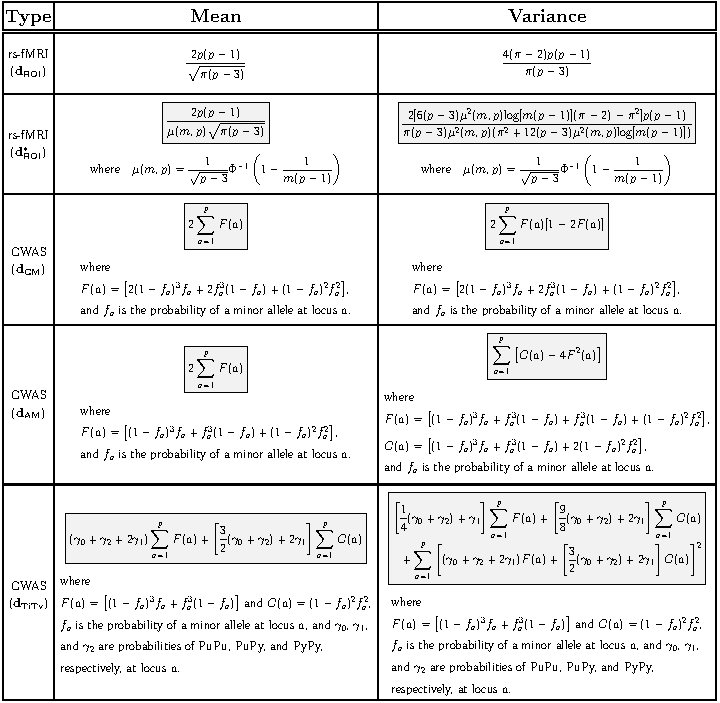
\includegraphics[width=\textwidth]{bioinformaticsy_tab.pdf}
%\end{table}

\begin{table}[H]
\caption{Summary of distance distribution derivations for standard normal and standard uniform data. Asymptotic estimates are given for both standard and max-min normalized q-metrics. These estimates are relevant for all $q \in \mathbb{N}$ and $p \geq 100$.}
\label{tab:dist_distr_general1}
\centering
% trim=left botm right top
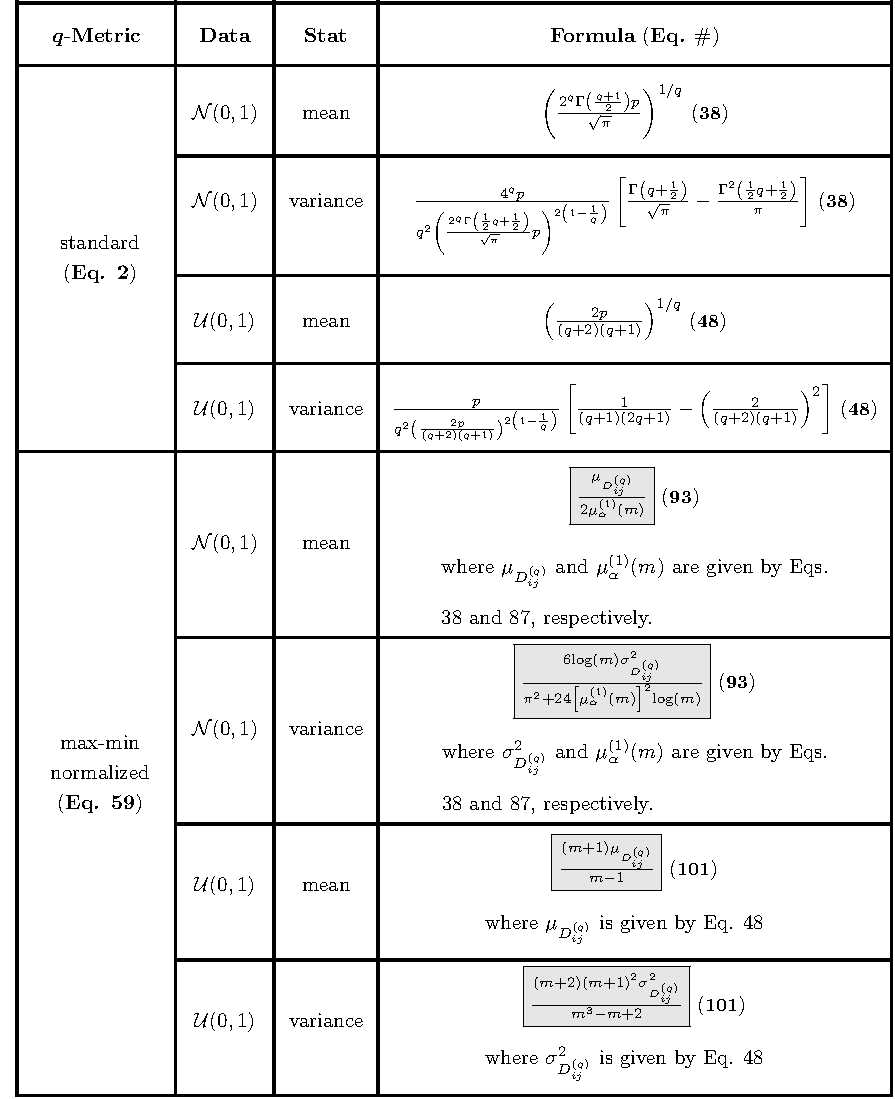
\includegraphics[clip,trim=0.27cm 0.0cm 0.0cm 0.05cm,width=\textwidth]{updated_distributions_table(5-23-2019).pdf}
\end{table}

\begin{table}[H]
	\caption{Asymptotic estimates for means and variances for the standard $L_1$ and $L_2$ distance distributions. Estimates for both standard normal and standard uniform data are given.}
	\label{tab:dist_distr_standardL1L2}
	\centering
	% trim=left botm right top
	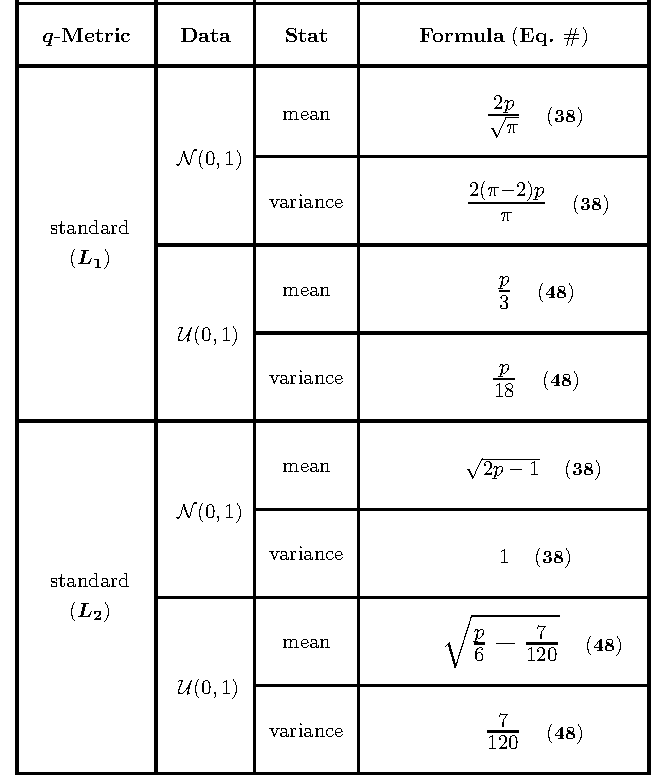
\includegraphics[clip,trim=0.27cm 0.0cm 0.0cm 0.05cm,width=0.7\textwidth]{updated_typical_metrics_table.pdf}
\end{table}

\begin{table}[H]
	\caption{Asymptotic estimates for means and variances for the max-min normalized $L_1$ and $L_2$ distance distributions. Estimates for both standard normal and standard uniform data are given.}
	\label{tab:dist_distr_normalizedL1L2}
	\centering
	% trim=left botm right top
	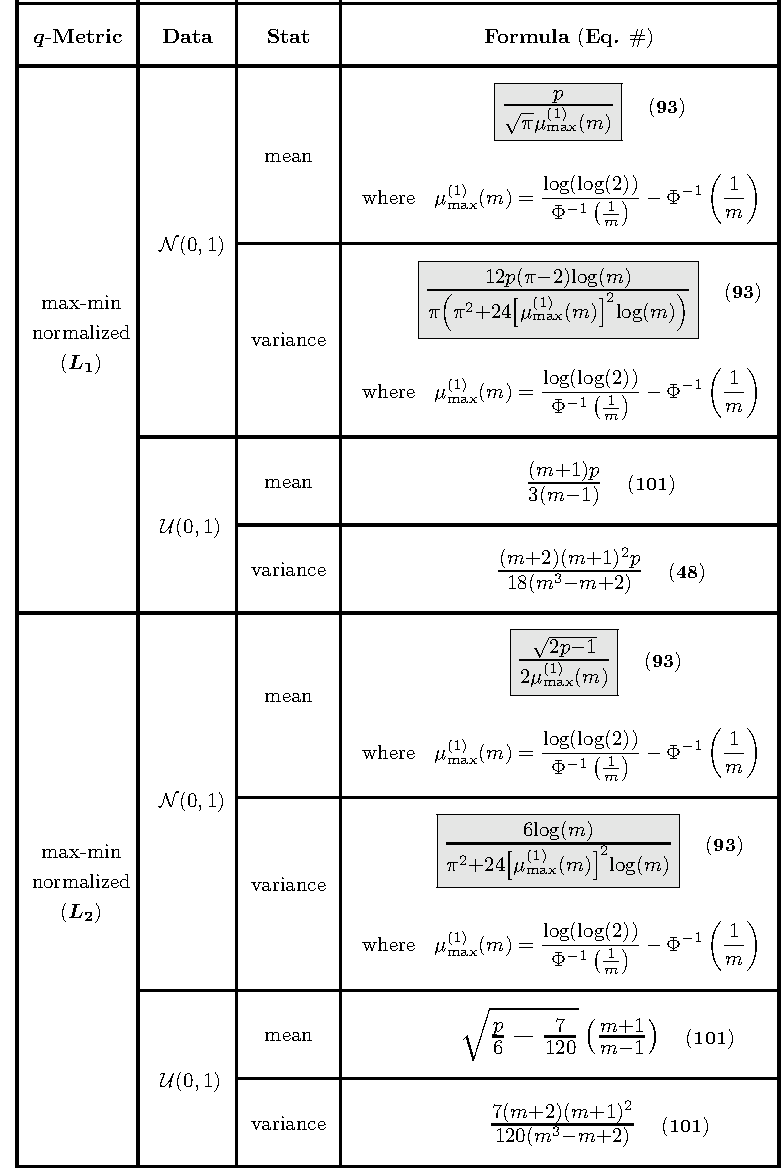
\includegraphics[clip,trim=0.27cm 0.0cm 0.0cm 0.05cm,width=0.85\textwidth]{updated_typical_metrics_table(normalized).pdf}
\end{table}

\begin{table}[H]
\caption{Summary of distance distribution derivations for GWAS data.}
\label{tab:dist_distr_gwas}
\centering
% trim=left botm right top
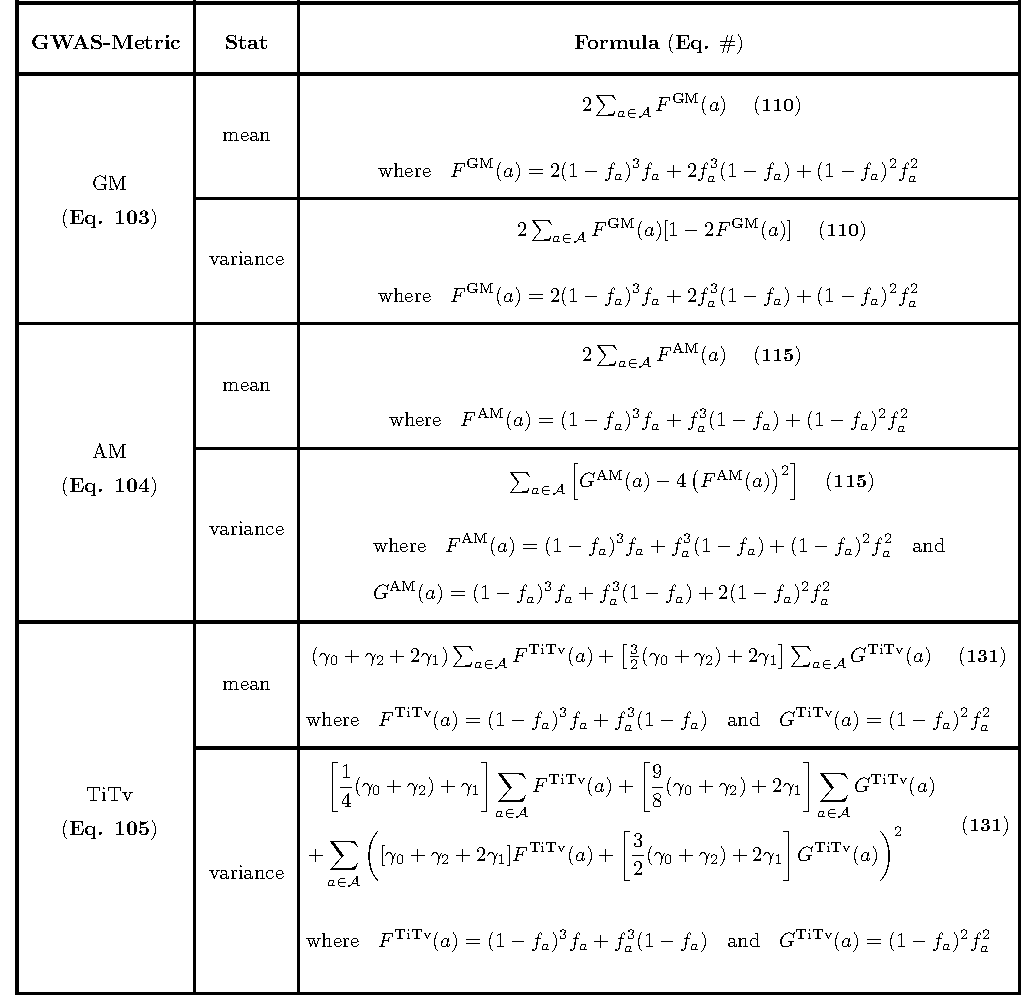
\includegraphics[clip,trim=0.27cm 0.0cm 0.0cm 0.05cm,width=\textwidth]{updated_distributions_table-gwas(5-23-2019).pdf}
\end{table}

\begin{table}[H]
\caption{Summary of distance distribution derivations for rs-fMRI data.}
\label{tab:dist_distr_rs-fMRI}
\centering
% trim=left botm right top
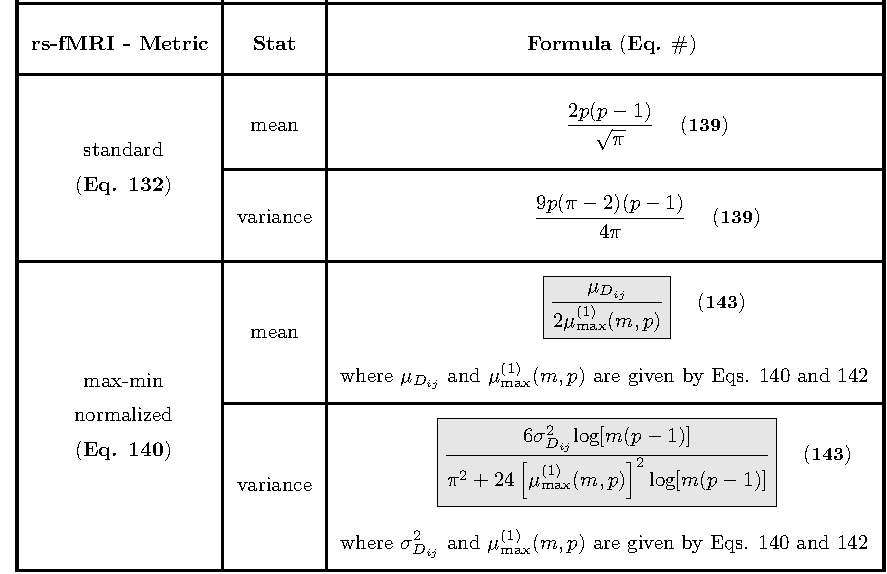
\includegraphics[clip,trim=0.27cm 0.0cm 0.0cm 0.05cm,width=\textwidth]{updated_distributions_table-rs-fMRI.pdf}
\end{table}

\bibliographystyle{unsrt}
\bibliography{BoD}   % name of bib file
\end{document}
